% Options for packages loaded elsewhere
\PassOptionsToPackage{unicode}{hyperref}
\PassOptionsToPackage{hyphens}{url}
\PassOptionsToPackage{dvipsnames,svgnames,x11names}{xcolor}
%
\documentclass[
  10pt,
]{article}
\usepackage{amsmath,amssymb}
\usepackage{iftex}
\ifPDFTeX
  \usepackage[T1]{fontenc}
  \usepackage[utf8]{inputenc}
  \usepackage{textcomp} % provide euro and other symbols
\else % if luatex or xetex
  \usepackage{unicode-math} % this also loads fontspec
  \defaultfontfeatures{Scale=MatchLowercase}
  \defaultfontfeatures[\rmfamily]{Ligatures=TeX,Scale=1}
\fi
\usepackage{lmodern}
\ifPDFTeX\else
  % xetex/luatex font selection
  \setmainfont[]{DejaVu Serif}
  \setsansfont[]{DejaVu Sans}
  \setmonofont[]{DejaVu Sans Mono}
  \setmathfont[]{Latin Modern Math}
\fi
% Use upquote if available, for straight quotes in verbatim environments
\IfFileExists{upquote.sty}{\usepackage{upquote}}{}
\IfFileExists{microtype.sty}{% use microtype if available
  \usepackage[]{microtype}
  \UseMicrotypeSet[protrusion]{basicmath} % disable protrusion for tt fonts
}{}
\makeatletter
\@ifundefined{KOMAClassName}{% if non-KOMA class
  \IfFileExists{parskip.sty}{%
    \usepackage{parskip}
  }{% else
    \setlength{\parindent}{0pt}
    \setlength{\parskip}{6pt plus 2pt minus 1pt}}
}{% if KOMA class
  \KOMAoptions{parskip=half}}
\makeatother
\usepackage{xcolor}
\usepackage[margin=2.0cm]{geometry}
\usepackage{color}
\usepackage{fancyvrb}
\newcommand{\VerbBar}{|}
\newcommand{\VERB}{\Verb[commandchars=\\\{\}]}
\DefineVerbatimEnvironment{Highlighting}{Verbatim}{commandchars=\\\{\}}
% Add ',fontsize=\small' for more characters per line
\newenvironment{Shaded}{}{}
\newcommand{\AlertTok}[1]{\textcolor[rgb]{1.00,0.00,0.00}{\textbf{#1}}}
\newcommand{\AnnotationTok}[1]{\textcolor[rgb]{0.38,0.63,0.69}{\textbf{\textit{#1}}}}
\newcommand{\AttributeTok}[1]{\textcolor[rgb]{0.49,0.56,0.16}{#1}}
\newcommand{\BaseNTok}[1]{\textcolor[rgb]{0.25,0.63,0.44}{#1}}
\newcommand{\BuiltInTok}[1]{\textcolor[rgb]{0.00,0.50,0.00}{#1}}
\newcommand{\CharTok}[1]{\textcolor[rgb]{0.25,0.44,0.63}{#1}}
\newcommand{\CommentTok}[1]{\textcolor[rgb]{0.38,0.63,0.69}{\textit{#1}}}
\newcommand{\CommentVarTok}[1]{\textcolor[rgb]{0.38,0.63,0.69}{\textbf{\textit{#1}}}}
\newcommand{\ConstantTok}[1]{\textcolor[rgb]{0.53,0.00,0.00}{#1}}
\newcommand{\ControlFlowTok}[1]{\textcolor[rgb]{0.00,0.44,0.13}{\textbf{#1}}}
\newcommand{\DataTypeTok}[1]{\textcolor[rgb]{0.56,0.13,0.00}{#1}}
\newcommand{\DecValTok}[1]{\textcolor[rgb]{0.25,0.63,0.44}{#1}}
\newcommand{\DocumentationTok}[1]{\textcolor[rgb]{0.73,0.13,0.13}{\textit{#1}}}
\newcommand{\ErrorTok}[1]{\textcolor[rgb]{1.00,0.00,0.00}{\textbf{#1}}}
\newcommand{\ExtensionTok}[1]{#1}
\newcommand{\FloatTok}[1]{\textcolor[rgb]{0.25,0.63,0.44}{#1}}
\newcommand{\FunctionTok}[1]{\textcolor[rgb]{0.02,0.16,0.49}{#1}}
\newcommand{\ImportTok}[1]{\textcolor[rgb]{0.00,0.50,0.00}{\textbf{#1}}}
\newcommand{\InformationTok}[1]{\textcolor[rgb]{0.38,0.63,0.69}{\textbf{\textit{#1}}}}
\newcommand{\KeywordTok}[1]{\textcolor[rgb]{0.00,0.44,0.13}{\textbf{#1}}}
\newcommand{\NormalTok}[1]{#1}
\newcommand{\OperatorTok}[1]{\textcolor[rgb]{0.40,0.40,0.40}{#1}}
\newcommand{\OtherTok}[1]{\textcolor[rgb]{0.00,0.44,0.13}{#1}}
\newcommand{\PreprocessorTok}[1]{\textcolor[rgb]{0.74,0.48,0.00}{#1}}
\newcommand{\RegionMarkerTok}[1]{#1}
\newcommand{\SpecialCharTok}[1]{\textcolor[rgb]{0.25,0.44,0.63}{#1}}
\newcommand{\SpecialStringTok}[1]{\textcolor[rgb]{0.73,0.40,0.53}{#1}}
\newcommand{\StringTok}[1]{\textcolor[rgb]{0.25,0.44,0.63}{#1}}
\newcommand{\VariableTok}[1]{\textcolor[rgb]{0.10,0.09,0.49}{#1}}
\newcommand{\VerbatimStringTok}[1]{\textcolor[rgb]{0.25,0.44,0.63}{#1}}
\newcommand{\WarningTok}[1]{\textcolor[rgb]{0.38,0.63,0.69}{\textbf{\textit{#1}}}}
\usepackage{longtable,booktabs,array}
\usepackage{calc} % for calculating minipage widths
% Correct order of tables after \paragraph or \subparagraph
\usepackage{etoolbox}
\makeatletter
\patchcmd\longtable{\par}{\if@noskipsec\mbox{}\fi\par}{}{}
\makeatother
% Allow footnotes in longtable head/foot
\IfFileExists{footnotehyper.sty}{\usepackage{footnotehyper}}{\usepackage{footnote}}
\makesavenoteenv{longtable}
\usepackage{graphicx}
\makeatletter
\def\maxwidth{\ifdim\Gin@nat@width>\linewidth\linewidth\else\Gin@nat@width\fi}
\def\maxheight{\ifdim\Gin@nat@height>\textheight\textheight\else\Gin@nat@height\fi}
\makeatother
% Scale images if necessary, so that they will not overflow the page
% margins by default, and it is still possible to overwrite the defaults
% using explicit options in \includegraphics[width, height, ...]{}
\setkeys{Gin}{width=\maxwidth,height=\maxheight,keepaspectratio}
% Set default figure placement to htbp
\makeatletter
\def\fps@figure{htbp}
\makeatother
\setlength{\emergencystretch}{3em} % prevent overfull lines
\providecommand{\tightlist}{%
  \setlength{\itemsep}{0pt}\setlength{\parskip}{0pt}}
\setcounter{secnumdepth}{-\maxdimen} % remove section numbering
% doc_header.tex -- LaTeX preamble additions used by build_docs.sh for every
% Markdown -> LaTeX -> PDF conversion (README and provenance documents of Revision_SuperLoop).
\usepackage{etoolbox}
% longtable may not be loaded by pandoc when a document has no table
\usepackage{longtable}
% bold vectors: \bm -> \symbf under unicode-math (XeLaTeX), bm package otherwise
\makeatletter
\@ifpackageloaded{unicode-math}{\providecommand{\bm}[1]{\symbf{#1}}}{\usepackage{bm}}
\makeatother
% smaller type in long tables so that wide audit tables fit the text width;
% inside a table a line break is allowed after an underscore of plain text
% (pandoc writes it as \_), so that long identifiers wrap inside their column
% rows are set a little apart, so that symbols with indices do not touch
\AtBeginEnvironment{longtable}{\footnotesize\renewcommand{\arraystretch}{1.45}%
  \let\sptunderscore\_\def\_{\sptunderscore\allowbreak}}
\setlength{\LTcapwidth}{\textwidth}
% A short table is kept on one page.  The build (code/scripts/keep_tables.py) ends the rows of such a table with \\*,
% which forbids a page break after a row, and sets \sptkeptpenalty to 10000 in front of the table.  This penalty is
% put here in the place of the breakpoint (penalty 0) that longtable leaves after every table, so that the paragraph
% that follows a kept table, its caption, begins on the same page; it is set back to 0 after the table.
\newcount\sptkeptpenalty
\sptkeptpenalty=0
\makeatletter
\patchcmd{\endlongtable}{\endgraf\penalty\z@\addvspace\LTpost}%
  {\endgraf\penalty\sptkeptpenalty\addvspace\LTpost\global\sptkeptpenalty=\z@}%
  {}{\PackageError{doc_header}{the end of longtable could not be patched}{The tables can still be typeset, but a short table may be separated from its caption.}}
\makeatother
% allow line breaks after slashes and hyphens inside table cells
\usepackage{xurl}
% code blocks: break over-long lines instead of running into the margin.
% Plain ``` blocks are typeset by pandoc as {verbatim}, highlighted ones
% (```bash) as {Highlighting}; both are re-declared as breakable fancyvrb
% environments.  The continuation line is marked with a small hooked arrow.
\usepackage{fvextra}
\RecustomVerbatimEnvironment{verbatim}{Verbatim}{breaklines,breakanywhere,fontsize=\small}
\makeatletter
\@ifundefined{Highlighting}{}{%
  \RecustomVerbatimEnvironment{Highlighting}{Verbatim}{breaklines,breakanywhere,fontsize=\small,commandchars=\\\{\}}}
\makeatother
% inline code (pandoc writes it as \texttt{...}): never hyphenate -- an inserted
% hyphen could be read as part of a file name -- but allow a line break after
% an underscore, slash, comma, colon or equals sign, so that long paths and
% column lists wrap inside the text width and inside table columns.
% Inside a formula (e.g. the name of a notebook symbol in an equation) the same
% command must first leave math mode, which \text of amsmath does.
\ExplSyntaxOn
\tl_new:N \l__spt_code_tl
\cs_new_protected:Npn \__spt_texttt:n #1
  {
    \tl_set:Nn \l__spt_code_tl {#1}
    \regex_replace_all:nnN { ([\/\,\:\=]) } { \1 \c{allowbreak} } \l__spt_code_tl
    \regex_replace_all:nnN { \c{_} } { \c{_} \c{allowbreak} } \l__spt_code_tl
    \group_begin: \ttfamily \hyphenchar \font = -1 \scan_stop: \l__spt_code_tl \group_end:
  }
\RenewDocumentCommand \texttt { m }
  {
    \mode_if_math:TF { \text { \__spt_texttt:n {#1} } } { \__spt_texttt:n {#1} }
  }
\ExplSyntaxOff
% A figure is written in the Markdown source as an image paragraph followed by
% a caption paragraph ("**Figure S1.** ..."), so that the caption is also
% visible on GitHub.  An image that starts a paragraph is centered.
\usepackage{graphicx}% pandoc loads it only for documents that contain an image
\NewCommandCopy\sptincludegraphics\includegraphics
\RenewDocumentCommand\includegraphics{O{} m}{%
  \ifvmode\begin{center}\sptincludegraphics[#1]{#2}\end{center}%
  \else\sptincludegraphics[#1]{#2}\fi}
% keep figures where they are referenced
\usepackage{float}
\floatplacement{figure}{H}
% running header with the document title
\usepackage{fancyhdr}
\pagestyle{fancy}
\fancyhf{}
\fancyhead[L]{\small PROJECT spacetimes, Revision\_SuperLoop}
\fancyhead[R]{\small\thepage}
\renewcommand{\headrulewidth}{0.4pt}
% 16x16 matrices: tighter columns so that a full matrix fits the text width
\setlength{\arraycolsep}{3.2pt}
% The documents of this project contain long tagged symbols, file paths and
% identifiers that cannot be hyphenated.  A paragraph is therefore allowed to
% have looser lines before TeX gives up and lets a line stick out of the margin.
\AtBeginDocument{\tolerance=2000 \emergencystretch=5em \hbadness=2000}
\ifLuaTeX
  \usepackage{selnolig}  % disable illegal ligatures
\fi
\IfFileExists{bookmark.sty}{\usepackage{bookmark}}{\usepackage{hyperref}}
\IfFileExists{xurl.sty}{\usepackage{xurl}}{} % add URL line breaks if available
\urlstyle{same}
\hypersetup{
  pdftitle={The superfluid boson singlet state by the method of Cornwall, Jackiw and Tomboulis},
  pdfauthor={Prepared for Patrick Lee Nash, Ph.D.},
  colorlinks=true,
  linkcolor={blue},
  filecolor={Maroon},
  citecolor={blue},
  urlcolor={blue},
  pdfcreator={LaTeX via pandoc}}

\title{The superfluid boson singlet state by the method of Cornwall,
Jackiw and Tomboulis}
\usepackage{etoolbox}
\makeatletter
\providecommand{\subtitle}[1]{% add subtitle to \maketitle
  \apptocmd{\@title}{\par {\large #1 \par}}{}{}
}
\makeatother
\subtitle{PROJECT spacetimes, Revision\_SuperLoop, folder test2. Stage
D: the creation of the superfluid boson singlet state from the spinor
field, with its provenance}
\author{Prepared for Patrick Lee Nash, Ph.D.}
\date{November 19, 2026}

\begin{document}
\maketitle

\hypertarget{the-task-and-the-result-in-brief}{%
\section{1. The task, and the result in
brief}\label{the-task-and-the-result-in-brief}}

\hypertarget{the-task}{%
\subsection{1.1 The task}\label{the-task}}

On November 18, 2026 the author added six stages to Test 2, named D to I
in this project. They ask for the superfluid boson singlet state (SFBS,
spin 0) of the spinor field to be treated by the method of J. M.
Cornwall, R. Jackiw and E. Tomboulis, Phys. Rev.~D 10, 2428 (1974),
called CJT below:

\begin{itemize}
\tightlist
\item
  \textbf{D.} apply the method of CJT to analyze, explain and discuss
  the creation of the SFBS from the spinor field;
\item
  \textbf{E.} derive the effective potential of the SFBS (the analogue
  of the Mexican-hat potential of the Higgs doublet);
\item
  \textbf{F.} find its relative minima and break the symmetry
  spontaneously;
\item
  \textbf{G.} expand the SFBS about a minimum (the approximation SFBSv);
\item
  \textbf{H.} derive the kinetic Lagrangian of the SFBS;
\item
  \textbf{I.} substitute SFBSv into the kinetic Lagrangian, diagonalize
  the mass terms, work out the surviving symmetry group and prove its
  relation to the group of electromagnetism and the massless photon.
\end{itemize}

\textbf{This document answers stage D.} Stages E to I are not yet
answered; they will be added to this document as further sections, each
when it is complete. On November 19, 2026 the author added: complete
stage D, resolve all issues, and invent mathematically possible fixes.
The issues are the four discrepancies between the method of CJT and the
earlier treatment of the SFBS in this project that the first
calculations of stage D had shown; they are stated in Section 6.3 and
resolved in Section 7.

\hypertarget{the-result-of-stage-d-in-brief}{%
\subsection{1.2 The result of stage D in
brief}\label{the-result-of-stage-d-in-brief}}

Units: the momentum cutoff \(\Lambda_{\rm LL}\) is 1. The numbers are
for the mass \(m_{\rm LL}=0.2\) of the spinor charges, the value used
throughout Test 2.

\begin{enumerate}
\def\labelenumi{\arabic{enumi}.}
\tightlist
\item
  \textbf{The method.} The effective action
  \(\Gamma^{\rm CJT}_{\rm LL}\) of CJT is a functional of the propagator
  of the spinor field. Because the SFBS is a pair of two spinor charges,
  the propagator is taken for the Nambu spinor, which holds the field
  and its conjugate; its ``pair'' part is the SFBS. In the two-loop
  approximation, the first one that contains the interaction,
  \(\Gamma^{\rm CJT}_{\rm LL}\) on a state that does not change in time
  equals minus the duration times the energy of a quasi-free state
  (Theorem D2), so that the approximation is a variational one. It
  contains three contractions of the interaction (Theorem D1): the
  pair-pair contraction, which the earlier treatment kept, and two equal
  normal contractions, which it dropped.
\item
  \textbf{What the normal contractions do.} They act in 64 normal
  channels with the coefficients of Table 1 (Theorem D3). On the vacuum
  they do two things: they shift the chemical potential by
  \(\tfrac32G_{\rm LL}N^\Lambda_{\rm LL}\), an effect of the order of
  the factors of the interaction (Theorem D4), and they dress the Dirac
  mass. With the interaction not ordered, the condensed vacuum has the
  Dirac mass \(4m^{\rm b}_{\rm LL}\), four times the mass
  \(m^{\rm b}_{\rm LL}\) of the Lagrangian, exactly (Theorem D5).
\item
  \textbf{The issues.} If 0.2 is read as the mass of the Lagrangian and
  the interaction is not ordered, the critical coupling is 32.3506
  instead of 21.28661, and the vacuum at the coupling 22.5 of Test 2 is
  normal, with the Dirac mass 0.539206, instead of condensed.
\item
  \textbf{The resolution.} The interaction is normal-ordered with
  respect to the normal correlations of the vacuum. This is the same as
  two counterterms, one for the chemical potential and one for the mass,
  fixed by two conditions: the vacuum is charge-symmetric at
  \(\mu_{\rm LL}=0\), and \(m_{\rm LL}\) is the Dirac mass of the vacuum
  (Theorem D6). The mass of the Lagrangian is then
  \(m^{\rm b}_{\rm LL}=m_{\rm LL}(1-3G_{\rm LL}/(4G^{\rm crit}_{\rm LL}))\)
  in the normal vacuum and \(m_{\rm LL}/4\) in the condensed one. With
  this reading the two-loop vacuum is the vacuum of the earlier
  treatment, with the same gap equation:
  \(G^{\rm crit}_{\rm LL}=21.28661\), and at \(G_{\rm LL}=22.5\) the gap
  \(\Delta^{\rm vac}_{\rm LL}=0.2094933\). An alternative that changes
  the interaction instead (its axially symmetric completion, Theorem D8)
  removes the dressing of the mass altogether; it is recorded and not
  adopted.
\item
  \textbf{The creation of the SFBS.} In the normal vacuum the pair part
  of the propagator has a pole below the threshold of two spinor charges
  when \(G^{\rm bd}_{\rm LL}<G_{\rm LL}<G^{\rm crit}_{\rm LL}\)
  (\(G^{\rm bd}_{\rm LL}=17.7463\)): the interaction binds two spinor
  charges into a boson of spin 0, the SFBS boson, with the mass
  \(M^{\rm B}_{\rm LL}\) given by
  \(G_{\rm LL}\chi^{\rm pr}_{\rm LL}(M^{\rm B}_{\rm LL},0)=1\) (Theorem
  D7). The normal channels do not mix with it. Its mass falls to zero at
  \(G^{\rm crit}_{\rm LL}\); above, the normal state is unstable, the
  pair field grows exponentially, and the SFBS condenses: the
  superfluid.
\item
  \textbf{Verified in real time.} The time-dependent equations of the
  two-loop action were integrated by CVODE. At \(G_{\rm LL}=20\) the
  pair amplitude rings with the frequency 0.279252; the predicted boson
  mass is 0.279252 (relative difference 1.0e-7). At \(G_{\rm LL}=22.5\)
  it grows with the rate 0.249607; the predicted rate is 0.249608
  (relative difference 6.2e-7).
\item
  \textbf{What remains different from the earlier treatment.} After the
  normal ordering the two treatments agree at the vacuum and to the
  first order around it. They differ at the second order: the normal
  stationary state above the critical coupling is itself dressed (Dirac
  mass 0.227347 at \(G_{\rm LL}=22.5\)), so that the condensed vacuum
  lies 3.8816e-5 below it instead of 5.2884e-5. This is a result of the
  fuller approximation, not an inconsistency; its consequences for the
  potential and for the masses belong to stages E to I.
\end{enumerate}

Every statement above is checked by the program \texttt{t2\_cjt} (checks
CJ-1 to CJ-11, all passed; Appendix A).

\hypertarget{how-to-read-this-document}{%
\subsection{1.3 How to read this
document}\label{how-to-read-this-document}}

The document is self-contained: every symbol is defined where it first
appears, and the complete table of the symbols of the folder is Appendix
C. Theorems are numbered D1 to D8; each is followed by its proof and by
the check of the program that verifies it by machine. Section 2 states
the model. Section 3 explains the method of CJT and its two-loop
approximation. Sections 4 to 6 work out what the approximation gives for
the model as it stands, and state the issues. Section 7 resolves them.
Section 8 is the creation of the SFBS. Section 9 discusses the limits of
the approximation.

\hypertarget{the-model}{%
\section{2. The model}\label{the-model}}

\hypertarget{the-field-and-its-matrices}{%
\subsection{2.1 The field and its
matrices}\label{the-field-and-its-matrices}}

The spinor field \(\Psi_{\rm LL}\) has 8 complex components on the
Minkowski space \(\mathbb R^{1,3}_{\rm LL}\) with the points
\(x_{\rm LL}=(x^0_{\rm LL},\vec x_{\rm LL})\), \(x^0_{\rm LL}\) the
time: a Dirac index with 4 values times an isospin index with 2 values
(up, down). The component with the Dirac index number 1 to 4 and the
isospin index number 1 or 2 has the number 2 (Dirac number \(-1\)) \(+\)
isospin number; \(\Psi_{{\rm LL},a}\) denotes one component, numbered by
its subscript, \(\Psi^\dagger_{\rm LL}\) the row of the Hermitian
conjugates, \(\Psi^T_{\rm LL}\) the row of the components themselves. A
matrix written as a tensor product, Dirac matrix \(\otimes\) isospin
matrix, acts on these 8 components.

The Dirac matrices are those of the chiral basis,
\[\gamma^0_{\rm LL}=\begin{pmatrix}0&\sigma^{\rm LL}_0\\\sigma^{\rm LL}_0&0\end{pmatrix},\qquad
\gamma^j_{\rm LL}=\begin{pmatrix}0&\sigma^{\rm LL}_j\\-\sigma^{\rm LL}_j&0\end{pmatrix}\quad(j=1,2,3),\tag{2.1}\]
with the \(2\times2\) unit matrix \(\sigma^{\rm LL}_0\) and the Pauli
matrices \(\sigma^{\rm LL}_j\). From them:
\(\beta_{\rm LL}=\gamma^0_{\rm LL}\),
\(\alpha^j_{\rm LL}=\gamma^0_{\rm LL}\gamma^j_{\rm LL}\), the chirality
matrix
\(\gamma^{\rm ch}_{\rm LL}=i\gamma^0_{\rm LL}\gamma^1_{\rm LL}\gamma^2_{\rm LL}\gamma^3_{\rm LL}\),
and the charge-conjugation matrix
\(C_{\rm LL}=i\gamma^2_{\rm LL}\gamma^0_{\rm LL}\), which is unitary and
obeys
\(C_{\rm LL}\gamma^p_{\rm LL}C_{\rm LL}^\dagger=-(\gamma^p_{\rm LL})^T\)
for \(p=0,1,2,3\). The Pauli matrices that act on the isospin index are
written \(\tau^{\rm LL}_\iota\) (\(\iota=1,2,3\)), and
\(\mathsf E_{\rm LL}=i\sigma^{\rm LL}_2=\begin{pmatrix}0&1\\-1&0\end{pmatrix}\).
The unit matrices of 2, 4, 8 and 16 rows are \(\mathsf 1_2\),
\(\mathsf 1_4\), \(\mathsf 1_8\), \(\mathsf 1_{16}\); a number added to
a matrix stands for that number times the unit matrix.

The \textbf{pair matrices} of the scalar channel are the three
\(8\times8\) matrices
\[\mathsf K^\iota_{\rm LL}=C_{\rm LL}\gamma^{\rm ch}_{\rm LL}\otimes\mathsf E_{\rm LL}\tau^{\rm LL}_\iota,\qquad\iota=1,2,3.\tag{2.2}\]
They are antisymmetric,
\((\mathsf K^\iota_{\rm LL})^T=-\mathsf K^\iota_{\rm LL}\), and unitary;
they are orthogonal to each other in the sense
\(\mathrm{tr}\big(\mathsf K^\iota_{\rm LL}(\mathsf K^{\iota'}_{\rm LL})^\dagger\big)=8\)
for \(\iota=\iota'\) and \(0\) otherwise. The \textbf{pair operators}
are
\[\Pi^\iota_{\rm LL}(x_{\rm LL})=\Psi^T_{\rm LL}\mathsf K^\iota_{\rm LL}\Psi_{\rm LL}
=\sum_{a,b}(\mathsf K^\iota_{\rm LL})_{ab}\Psi_{{\rm LL},a}\Psi_{{\rm LL},b},\tag{2.3}\]
both fields at the point \(x_{\rm LL}\). \(\Pi^\iota_{\rm LL}\) removes
two spinor charges at one point. It is a Lorentz scalar: in each of the
two chirality blocks of the chiral basis the Dirac factor
\(C_{\rm LL}\gamma^{\rm ch}_{\rm LL}\) is \(-\mathsf E_{\rm LL}\), the
antisymmetric combination of the two spin states, so that the two spins
form the singlet (total spin 0); this is the ``singlet'' and the
``\(S^{\rm sp}_{\rm LL}=0\)'' (spin zero) of the name SFBS. Because the
components of the field anticommute, the isospin factor of an
antisymmetric pair matrix with an antisymmetric spin factor must be
symmetric: \(\mathsf E_{\rm LL}\tau^{\rm LL}_\iota\) are the three
symmetric \(2\times2\) matrices, and the pair is an isospin triplet. The
three operators \(\Pi^\iota_{\rm LL}\) are the components of an isospin
vector.

\hypertarget{the-lagrangian-and-the-hamiltonian}{%
\subsection{2.2 The Lagrangian and the
Hamiltonian}\label{the-lagrangian-and-the-hamiltonian}}

The Lagrangian density of the spinor field with its attractive contact
interaction, without gauge fields (they are not needed before stage I),
is
\[\mathcal L^{\rm c}_{\rm LL}=\bar\Psi_{\rm LL}\big(i\gamma^p_{\rm LL}\partial_p-m^{\rm b}_{\rm LL}\big)\Psi_{\rm LL}
+\mu^{\rm b}_{\rm LL}\Psi^\dagger_{\rm LL}\Psi_{\rm LL}
+\tfrac14G_{\rm LL}\sum_\iota(\Pi^\iota_{\rm LL})^\dagger\Pi^\iota_{\rm LL},\tag{2.4}\]
with \(\bar\Psi_{\rm LL}=\Psi^\dagger_{\rm LL}\beta_{\rm LL}\),
\(\partial_p\) the derivative with respect to \(x^p_{\rm LL}\) (summed
over \(p=0,\dots,3\)), the coupling \(G_{\rm LL}>0\), a mass and a
chemical potential. The action is
\(\mathcal S^{\rm sf}_{\rm LL}=\int d^4x_{\rm LL}\,\mathcal L^{\rm c}_{\rm LL}\),
and \(\mathcal S^{\rm int}_{\rm LL}\) is its last term. The Hamiltonian
density that belongs to (2.4) is
\[\mathcal H^{\rm sf}_{\rm LL}=\Psi^\dagger_{\rm LL}\big(\mathsf h_{\rm LL}-\mu^{\rm b}_{\rm LL}\big)\Psi_{\rm LL}
-\tfrac14G_{\rm LL}\sum_\iota(\Pi^\iota_{\rm LL})^\dagger\Pi^\iota_{\rm LL},\qquad
\mathsf h_{\rm LL}(\vec q_{\rm LL})=\sum_j\alpha^j_{\rm LL}q^j_{\rm LL}+\beta_{\rm LL}m^{\rm b}_{\rm LL},\tag{2.5}\]
where \(\mathsf h_{\rm LL}(\vec q_{\rm LL})\) (times \(\mathsf 1_2\) on
the isospin index) is the matrix of the free Hamiltonian on a plane wave
of the momentum \(\vec q_{\rm LL}\); its eigenvalues are
\(\pm(q_{\rm LL}^2+(m^{\rm b}_{\rm LL})^2)^{1/2}\), four times each.

\textbf{The cutoff.} A contact interaction needs a cutoff. As everywhere
in Test 2 the field contains only the plane waves with
\(q_{\rm LL}<\Lambda_{\rm LL}\). The anticommutator of
\(\Psi_{{\rm LL},a}(\vec x_{\rm LL})\) with
\(\Psi^\dagger_{{\rm LL},b}(\vec x'_{\rm LL})\) at equal times is then
zero for two different components and, for one and the same component,
the function
\(\int_{q_{\rm LL}<\Lambda_{\rm LL}}d^3q_{\rm LL}(2\pi)^{-3}\exp\big(i\vec q_{\rm LL}\cdot(\vec x_{\rm LL}-\vec x'_{\rm LL})\big)\),
whose value at coinciding points is
\[N^\Lambda_{\rm LL}=\int_{q_{\rm LL}<\Lambda_{\rm LL}}\frac{d^3q_{\rm LL}}{(2\pi)^3}=\frac{\Lambda_{\rm LL}^3}{6\pi^2}=0.0168869\ \ (\Lambda_{\rm LL}=1),\tag{2.6}\]
the number of modes per volume and per component of the field.

\textbf{The order of the factors, and the name ``bare''.} The Lagrangian
(2.4) treats the components of the field as anticommuting numbers and
does not say in which order the four field operators of the interaction
stand in the Hamiltonian. In (2.5) the order is fixed as written:
\((\Pi^\iota_{\rm LL})^\dagger\) to the left of \(\Pi^\iota_{\rm LL}\).
The mass and the chemical potential that stand in the Hamiltonian with
this order, and with nothing subtracted from the interaction, are called
the \textbf{bare} mass \(m^{\rm b}_{\rm LL}\) and the bare chemical
potential \(\mu^{\rm b}_{\rm LL}\). The symbols \(m_{\rm LL}\) and
\(\mu_{\rm LL}\) without the superscript are kept for the mass of the
spinor charges and for the chemical potential measured from the
charge-symmetric point; Sections 5 and 7 show how they are related to
the bare ones.

\hypertarget{the-symmetries}{%
\subsection{2.3 The symmetries}\label{the-symmetries}}

The Hamiltonian (2.5) is invariant under the rotations of space and
under parity; under the fermion-number transformations
\(\Psi_{\rm LL}\mapsto\exp(i\theta^{\rm F}_{\rm LL})\Psi_{\rm LL}\) with
a constant phase (the group \(U(1)^{\rm F}_{\rm LL}\)), which multiply
\(\Pi^\iota_{\rm LL}\) by \(\exp(2i\theta^{\rm F}_{\rm LL})\): a pair
carries the fermion number 2; and under the isospin rotations
\(SU(2)_{\rm v}\) of the isospin index, which rotate the three
\(\Pi^\iota_{\rm LL}\) as a vector. A fourth symmetry, the exchange of
particles and holes, is the subject of Section 5.

\hypertarget{what-the-creation-of-the-sfbs-means}{%
\subsection{2.4 What ``the creation of the SFBS''
means}\label{what-the-creation-of-the-sfbs-means}}

Three things are meant, and Section 8 establishes each of them with the
method of CJT:

\begin{enumerate}
\def\labelenumi{\arabic{enumi}.}
\tightlist
\item
  the SFBS as an operator: the pair operators (2.3), a composite boson
  field made of two spinor fields at one point;
\item
  the SFBS as a particle: a bound state of two spinor charges that the
  interaction creates, seen as a pole of the pair part of the
  propagator, with a mass below the threshold of two free spinor
  charges;
\item
  the SFBS as a condensate: above a critical coupling the mass of that
  particle has fallen to zero, the vacuum without pairs is unstable, and
  the pair operators acquire an expectation value. Its size is measured
  by the \textbf{order parameter}
  \[d^\iota_{\rm LL}=-\tfrac12G_{\rm LL}\langle\Pi^\iota_{\rm LL}\rangle,\qquad\vec d_{\rm LL}=(d^1_{\rm LL},d^2_{\rm LL},d^3_{\rm LL})\in\mathbb C^3,\tag{2.7}\]
  whose modulus is the gap
  \(\Delta_{\rm LL}=\lvert\vec d_{\rm LL}\rvert\) of a state with
  \(\vec d_{\rm LL}\times\vec d^{\,*}_{\rm LL}=0\) (a unitary state;
  \(\zeta_{\rm LL}=\lvert\vec d_{\rm LL}\times\vec d^{\,*}_{\rm LL}\rvert/\lvert\vec d_{\rm LL}\rvert^2\)
  measures the deviation from it).
\end{enumerate}

\hypertarget{the-method-of-cornwall-jackiw-and-tomboulis}{%
\section{3. The method of Cornwall, Jackiw and
Tomboulis}\label{the-method-of-cornwall-jackiw-and-tomboulis}}

\hypertarget{the-effective-action-of-the-propagator}{%
\subsection{3.1 The effective action of the
propagator}\label{the-effective-action-of-the-propagator}}

The usual effective action is a functional of the expectation value of a
field, and its stationary points are the possible vacua. A spinor field
has no expectation value. What can condense is a product of two spinor
fields, and the expectation value of a product of two fields is a
propagator. CJT therefore construct an effective action whose argument
is the propagator itself. For the present model the construction is as
follows.

\emph{The Nambu spinor.} The SFBS is a product of two fields
\(\Psi_{\rm LL}\) without a conjugate. To have such products inside one
propagator, the field and its conjugate are put into one column of 16
components,
\[\mathcal N_{\rm LL}(x_{\rm LL})=\begin{pmatrix}\Psi_{\rm LL}(x_{\rm LL})\\(\Psi^\dagger_{\rm LL}(x_{\rm LL}))^T\end{pmatrix},\tag{3.1}\]
the Nambu spinor; in momentum space its part of the momentum
\(\vec q_{\rm LL}\) is
\(\mathcal N_{\rm LL}(\vec q_{\rm LL})=(\Psi_{\rm LL}(\vec q_{\rm LL}),\Psi^\dagger_{\rm LL}(-\vec q_{\rm LL})^T)\).

\emph{The propagator.} It is the \(16\times16\) matrix function of two
points
\[i\,\mathcal G_{\rm LL}(x_{\rm LL},x'_{\rm LL})=\big\langle\mathrm T\,\mathcal N_{\rm LL}(x_{\rm LL})\,\mathcal N_{\rm LL}(x'_{\rm LL})^\dagger\big\rangle,\tag{3.2}\]
where \(\mathrm T\) puts the factor with the later time to the left,
with a minus sign if it exchanges the two. Its two diagonal \(8\times8\)
blocks are the ordinary propagators of particles and of holes. Its
off-diagonal blocks contain
\(\langle\Psi_{\rm LL}\Psi^T_{\rm LL}\rangle\) and
\(\langle\Psi^{\dagger T}_{\rm LL}\Psi^\dagger_{\rm LL}\rangle\): they
vanish unless pairs have condensed, and they are the place of the SFBS
in the method.

\emph{The source and the Legendre transform.} A source
\(\mathcal K^{\rm src}_{\rm LL}(x_{\rm LL},x'_{\rm LL})\), a
\(16\times16\) matrix function of two points, is coupled to the product
of two fields: the term
\(\tfrac12\int d^4x_{\rm LL}\,d^4x'_{\rm LL}\,\mathcal N_{\rm LL}(x_{\rm LL})^\dagger\mathcal K^{\rm src}_{\rm LL}(x_{\rm LL},x'_{\rm LL})\mathcal N_{\rm LL}(x'_{\rm LL})\)
is added to the action. The vacuum amplitude in the presence of the
source defines the generating functional by (vacuum amplitude)
\(=\exp(iW^{\rm src}_{\rm LL})\). The derivative of
\(W^{\rm src}_{\rm LL}\) with respect to the source is, up to a factor,
the propagator in the presence of the source. The effective action
\(\Gamma^{\rm CJT}_{\rm LL}[\mathcal G_{\rm LL}]\) is the Legendre
transform: \(W^{\rm src}_{\rm LL}\) minus the source times this
derivative (summed over the indices and integrated over the two points),
with the source expressed through the propagator. From this definition
follow the two properties that are used:

\begin{itemize}
\tightlist
\item
  the derivative of \(\Gamma^{\rm CJT}_{\rm LL}\) with respect to
  \(\mathcal G_{\rm LL}\) is proportional to the source. The theory
  itself is the case of no source: \textbf{the propagator of the theory
  makes \(\Gamma^{\rm CJT}_{\rm LL}\) stationary};
\item
  at such a stationary point
  \(\Gamma^{\rm CJT}_{\rm LL}=W^{\rm src}_{\rm LL}\) at vanishing
  source, and for a state that does not change in time this is
  \textbf{minus the duration times the energy} of the state.
\end{itemize}

\emph{The formula of CJT.} CJT prove that the effective action is
\[\Gamma^{\rm CJT}_{\rm LL}[\mathcal G_{\rm LL}]=-\tfrac i2\,\mathrm{Tr}\ln\mathcal G_{\rm LL}^{-1}
-\tfrac i2\,\mathrm{Tr}\big((\mathcal G^{\rm fr}_{\rm LL})^{-1}\mathcal G_{\rm LL}-1\big)
+\Gamma^{\rm 2PI}_{\rm LL}[\mathcal G_{\rm LL}]+\text{constant},\tag{3.3}\]
where \(\mathcal G^{\rm fr}_{\rm LL}\) is the propagator without
interaction, \(\mathrm{Tr}\) is the trace over the 16 components
together with the integral over the points, and
\(\Gamma^{\rm 2PI}_{\rm LL}\) is the sum of all vacuum graphs that stay
connected when any two of their lines are cut (two-particle-irreducible
graphs), drawn with the vertices of the interaction and with the
\emph{full} propagator \(\mathcal G_{\rm LL}\) as lines. The factor
\(\tfrac12\) in the first two terms, compared with the formula for a
Dirac field, counts every mode once although it occurs twice in the
Nambu spinor; the overall sign is the one of fermions. For a state that
is the same at every point and at every time, \(\mathcal G_{\rm LL}\)
depends on the difference of its two points only, and \(\mathrm{Tr}\)
becomes the duration times the volume times
\(\int d\omega^{\rm f}_{\rm LL}(2\pi)^{-1}\int d^3q_{\rm LL}(2\pi)^{-3}\,\mathrm{tr}\),
with the frequency \(\omega^{\rm f}_{\rm LL}\) conjugate to the time
difference.

\emph{Why this suits the problem.} The stationarity condition of (3.3)
is an equation for the whole propagator, pair part included. A solution
with a non-zero pair part is a condensate of the SFBS; the second
derivative of (3.3) at a solution governs the small oscillations of the
propagator about it, and a pole of these oscillations in the pair part
is the SFBS as a particle. No auxiliary boson field has to be introduced
by hand.

\hypertarget{the-two-loop-approximation-and-wicks-theorem}{%
\subsection{3.2 The two-loop approximation, and Wick's
theorem}\label{the-two-loop-approximation-and-wicks-theorem}}

\(\Gamma^{\rm 2PI}_{\rm LL}\) is a series in the number of loops. Its
first term has one vertex of the interaction and two closed lines (two
loops): it is the expectation value of \(\mathcal S^{\rm int}_{\rm LL}\)
in which the four field operators are contracted in pairs with the
propagator \(\mathcal G_{\rm LL}\) in all possible ways. This is the
approximation of this document. Since the vertex joins four fields at
one point and one time, only the propagator at coinciding points and
equal times enters, that is, the correlation matrices of the state: for
a state that is the same at every point,
\[(\mathsf C^{\rm n}_{\rm LL})_{ab}=\langle\Psi^\dagger_{{\rm LL},b}\Psi_{{\rm LL},a}\rangle,\qquad
(\mathsf C^{\rm p}_{\rm LL})_{ab}=\langle\Psi_{{\rm LL},a}\Psi_{{\rm LL},b}\rangle,\tag{3.4}\]
both fields at the same point and time: the normal correlation matrix
(Hermitian) and the pair correlation matrix (antisymmetric), each
\(8\times8\). With an argument,
\(\mathsf C^{\rm n}_{\rm LL}(\vec q_{\rm LL})\) and
\(\mathsf C^{\rm p}_{\rm LL}(\vec q_{\rm LL})\) are their parts of one
momentum,
\(\mathsf C^{\rm n}_{\rm LL}=\int_{q_{\rm LL}<\Lambda_{\rm LL}}d^3q_{\rm LL}(2\pi)^{-3}\mathsf C^{\rm n}_{\rm LL}(\vec q_{\rm LL})\)
and the same for \(\mathsf C^{\rm p}_{\rm LL}\). The order of the
operators in (3.4), the conjugate field to the left, is the order of the
interaction in (2.5).

\textbf{Theorem D1 (the three contractions).} In a state in which the
expectation value of a product of four field operators is the sum of the
products of the expectation values of pairs, with the signs of Wick's
theorem (a quasi-free state),
\[\Big\langle\sum_\iota(\Pi^\iota_{\rm LL})^\dagger\Pi^\iota_{\rm LL}\Big\rangle
=\sum_\iota\lvert\langle\Pi^\iota_{\rm LL}\rangle\rvert^2
+2\sum_\iota\mathrm{tr}\big(\mathsf K^\iota_{\rm LL}\mathsf C^{\rm n}_{\rm LL}(\mathsf K^\iota_{\rm LL})^\dagger(\mathsf C^{\rm n}_{\rm LL})^T\big),
\qquad\langle\Pi^\iota_{\rm LL}\rangle=\sum_{a,b}(\mathsf K^\iota_{\rm LL})_{ab}(\mathsf C^{\rm p}_{\rm LL})_{ab}.\tag{3.5}\]

\emph{Proof.} Write \(\mathsf K\) for one of the pair matrices in this
proof, with the entries \(\mathsf K_{ab}\); then
\((\Pi_{\rm LL})^\dagger\Pi_{\rm LL}=\sum\mathsf K^*_{ab}\mathsf K_{a'b'}\Psi^\dagger_{{\rm LL},b}\Psi^\dagger_{{\rm LL},a}\Psi_{{\rm LL},a'}\Psi_{{\rm LL},b'}\),
summed over the four indices. Wick's theorem gives three terms for the
expectation value of the four operators:
\(\langle\Psi^\dagger_{{\rm LL},b}\Psi^\dagger_{{\rm LL},a}\rangle\langle\Psi_{{\rm LL},a'}\Psi_{{\rm LL},b'}\rangle\),
minus
\(\langle\Psi^\dagger_{{\rm LL},b}\Psi_{{\rm LL},a'}\rangle\langle\Psi^\dagger_{{\rm LL},a}\Psi_{{\rm LL},b'}\rangle\),
plus
\(\langle\Psi^\dagger_{{\rm LL},b}\Psi_{{\rm LL},b'}\rangle\langle\Psi^\dagger_{{\rm LL},a}\Psi_{{\rm LL},a'}\rangle\).
The first is
\((\mathsf C^{\rm p}_{\rm LL})^*_{ab}(\mathsf C^{\rm p}_{\rm LL})_{a'b'}\);
summed with the two pair matrices it is
\(\lvert\sum\mathsf K_{ab}(\mathsf C^{\rm p}_{\rm LL})_{ab}\rvert^2\).
The third is
\((\mathsf C^{\rm n}_{\rm LL})_{b'b}(\mathsf C^{\rm n}_{\rm LL})_{a'a}\);
summed, it is
\(\sum\mathsf K_{a'b'}(\mathsf C^{\rm n}_{\rm LL})_{b'b}(\mathsf K^\dagger)_{ba}((\mathsf C^{\rm n}_{\rm LL})^T)_{aa'} =\mathrm{tr}(\mathsf K\mathsf C^{\rm n}_{\rm LL}\mathsf K^\dagger(\mathsf C^{\rm n}_{\rm LL})^T)\).
The second is
\(-(\mathsf C^{\rm n}_{\rm LL})_{a'b}(\mathsf C^{\rm n}_{\rm LL})_{b'a}\);
exchanging the names of the last two summation indices and using that
the pair matrix is antisymmetric turns it into the third.
\(\blacksquare\)

\emph{Check CJ-1} verifies (3.5) in the Fock space of 8 fermion modes
for the ground states of random quadratic Hamiltonians with pairing
(difference below \(10^{-13}\)), and with it the sign conventions of all
that follows.

The first term of (3.5) is the \textbf{pair-pair contraction}; the
second, the two equal \textbf{normal contractions}. The earlier
treatment of the SFBS in this project (a Hubbard-Stratonovich
transformation that introduces the pair field alone, followed by the
mean-field evaluation) kept the first term only. The method of CJT has
no such freedom: at two loops all three contractions belong to the same
graph.

\hypertarget{the-two-loop-action-is-the-energy-of-a-quasi-free-state}{%
\subsection{3.3 The two-loop action is the energy of a quasi-free
state}\label{the-two-loop-action-is-the-energy-of-a-quasi-free-state}}

\emph{The trial family.} Take any Hermitian \(8\times8\) matrix
\(\mathsf N^{\rm sc}_{\rm LL}\) and any antisymmetric \(8\times8\)
matrix \(\mathsf P_{\rm LL}\), and form the \(16\times16\)
\textbf{mean-field matrix}
\[\mathsf H^{\rm var}_{\rm LL}(\vec q_{\rm LL})=\begin{pmatrix}\mathsf h_{\rm LL}(\vec q_{\rm LL})+\mathsf N^{\rm sc}_{\rm LL}-\mu^{\rm b}_{\rm LL}&\mathsf P_{\rm LL}\\
\mathsf P_{\rm LL}^\dagger&-\big(\mathsf h_{\rm LL}(-\vec q_{\rm LL})+\mathsf N^{\rm sc}_{\rm LL}-\mu^{\rm b}_{\rm LL}\big)^T\end{pmatrix}.\tag{3.6}\]
It is the matrix of the quadratic Hamiltonian
\(\tfrac12\int d^3q_{\rm LL}(2\pi)^{-3}\mathcal N_{\rm LL}(\vec q_{\rm LL})^\dagger\mathsf H^{\rm var}_{\rm LL}(\vec q_{\rm LL})\mathcal N_{\rm LL}(\vec q_{\rm LL})\).
The propagator of the ground state of this Hamiltonian is
\(\mathcal G_{\rm LL}(\omega^{\rm f}_{\rm LL},\vec q_{\rm LL})=(\omega^{\rm f}_{\rm LL}-\mathsf H^{\rm var}_{\rm LL}(\vec q_{\rm LL}))^{-1}\),
with the rule that the poles at positive eigenvalues lie just below the
real axis and those at negative eigenvalues just above. The ground state
is quasi-free, and its \textbf{density matrix of the Nambu spinor}, the
\(16\times16\) matrix \(\mathsf R^{\rm Nb}_{\rm LL}(\vec q_{\rm LL})\)
with the entries
\(\langle\mathcal N^\dagger_{{\rm LL},b}\mathcal N_{{\rm LL},a}\rangle\),
is the projector on the eigenvectors of
\(\mathsf H^{\rm var}_{\rm LL}(\vec q_{\rm LL})\) with negative
eigenvalues,
\[\mathsf R^{\rm Nb}_{\rm LL}=\tfrac12\big(\mathsf 1_{16}-\mathrm{sgn}\,\mathsf H^{\rm var}_{\rm LL}\big)
=\begin{pmatrix}\mathsf C^{\rm n}_{\rm LL}(\vec q_{\rm LL})&-\mathsf C^{\rm p}_{\rm LL}(\vec q_{\rm LL})\\\cdot&\cdot\end{pmatrix},\tag{3.7}\]
where \(\mathrm{sgn}\) of a Hermitian matrix has the same eigenvectors
and the signs of the eigenvalues as eigenvalues (the lower blocks,
marked by dots, repeat the upper ones: the lower right block is
\(\mathsf 1_8-\mathsf C^{\rm n}_{\rm LL}(-\vec q_{\rm LL})^T\)). These
propagators, for all \(\mathsf N^{\rm sc}_{\rm LL}\) and
\(\mathsf P_{\rm LL}\), are the trial family.

\textbf{Theorem D2 (two loops = energy of a quasi-free state).} (a) On
the trial family, the effective action (3.3) with the two-loop term for
\(\Gamma^{\rm 2PI}_{\rm LL}\) is, per duration and volume and up to a
constant that is the same for the whole family, minus the functional
\[\begin{aligned}\mathcal E^{\rm var}_{\rm LL}={}&\int_{q_{\rm LL}<\Lambda_{\rm LL}}\frac{d^3q_{\rm LL}}{(2\pi)^3}\mathrm{tr}\big(\mathsf h_{\rm LL}(\vec q_{\rm LL})\mathsf C^{\rm n}_{\rm LL}(\vec q_{\rm LL})\big)
-\mu^{\rm b}_{\rm LL}\mathrm{tr}\,\mathsf C^{\rm n}_{\rm LL}\\
&-\tfrac14G_{\rm LL}\sum_\iota\lvert\langle\Pi^\iota_{\rm LL}\rangle\rvert^2
-\tfrac12G_{\rm LL}\sum_\iota\mathrm{tr}\big(\mathsf K^\iota_{\rm LL}\mathsf C^{\rm n}_{\rm LL}(\mathsf K^\iota_{\rm LL})^\dagger(\mathsf C^{\rm n}_{\rm LL})^T\big),\end{aligned}\tag{3.8}\]
and \(\mathcal E^{\rm var}_{\rm LL}\) is the expectation value of the
Hamiltonian density (2.5) in the trial state: the energy per volume. (b)
Every propagator that makes the two-loop action stationary, among all
propagators that are the same at every point and time, belongs to the
trial family, with the mean fields
\[\mathsf N^{\rm sc}_{\rm LL}=-G_{\rm LL}\sum_\iota(\mathsf K^\iota_{\rm LL})^\dagger(\mathsf C^{\rm n}_{\rm LL})^T\mathsf K^\iota_{\rm LL},\qquad
\mathsf P_{\rm LL}=\sum_\iota d^\iota_{\rm LL}(\mathsf K^\iota_{\rm LL})^\dagger,\qquad d^\iota_{\rm LL}=-\tfrac12G_{\rm LL}\langle\Pi^\iota_{\rm LL}\rangle\tag{3.9}\]
computed from its own correlation matrices (self-consistency). (c)
Consequently the two-loop approximation is variational: for every member
of the family, \(\mathcal E^{\rm var}_{\rm LL}\) times the volume is not
below the exact ground energy of the Hamiltonian.

\emph{Proof.} (a) The three terms of (3.3) are evaluated in turn.
\(\mathsf H^{\rm var}_{\rm LL}[0]\) denotes the matrix (3.6) with
\(\mathsf N^{\rm sc}_{\rm LL}=0\) and \(\mathsf P_{\rm LL}=0\), so that
\((\mathcal G^{\rm fr}_{\rm LL})^{-1}=\omega^{\rm f}_{\rm LL}-\mathsf H^{\rm var}_{\rm LL}[0]\);
all statements are per duration and volume. The frequency integrals are
taken along the imaginary axis,
\(\omega^{\rm f}_{\rm LL}=i\upsilon^{\rm f}_{\rm LL}\) with real
\(\upsilon^{\rm f}_{\rm LL}\): with the rule for the poles stated above,
turning the path of integration from the real to the imaginary axis
crosses no pole. One property of (3.6) is used throughout: because
\(\mathsf P_{\rm LL}\) is antisymmetric, exchanging the upper and the
lower 8 components turns the transpose of
\(\mathsf H^{\rm var}_{\rm LL}(\vec q_{\rm LL})\) into
\(-\mathsf H^{\rm var}_{\rm LL}(-\vec q_{\rm LL})\). Hence the
eigenvalues at \(-\vec q_{\rm LL}\) are minus those at
\(\vec q_{\rm LL}\): taken over all momenta the spectrum is symmetric
about zero, and the integral of the trace of
\(\mathsf H^{\rm var}_{\rm LL}\) over the momenta vanishes. The modulus
of a Hermitian matrix, written with bars, is the matrix with the same
eigenvectors and the moduli of the eigenvalues.

\emph{First term.}
\(-\tfrac i2\int d\omega^{\rm f}_{\rm LL}(2\pi)^{-1}\mathrm{tr}\ln(\omega^{\rm f}_{\rm LL}-\mathsf H^{\rm var}_{\rm LL}) =\tfrac12\int d\upsilon^{\rm f}_{\rm LL}(2\pi)^{-1}\mathrm{tr}\ln(i\upsilon^{\rm f}_{\rm LL}-\mathsf H^{\rm var}_{\rm LL})\).
By the symmetry of the spectrum, under the integral over the momenta
\(\mathrm{tr}\ln(i\upsilon^{\rm f}_{\rm LL}-\mathsf H^{\rm var}_{\rm LL})\)
may be replaced by
\(\tfrac12\mathrm{tr}\ln\big((\upsilon^{\rm f}_{\rm LL})^2+(\mathsf H^{\rm var}_{\rm LL})^2\big)\)
plus a constant. The elementary integral
\[\int_{-\infty}^{\infty}\frac{d\upsilon^{\rm f}_{\rm LL}}{2\pi}\Big(\mathrm{tr}\ln\big((\upsilon^{\rm f}_{\rm LL})^2+(\mathsf H^{\rm var}_{\rm LL})^2\big)-\mathrm{tr}\ln\big((\upsilon^{\rm f}_{\rm LL})^2+(\mathsf H^{\rm var}_{\rm LL}[0])^2\big)\Big)
=\mathrm{tr}\,\lvert\mathsf H^{\rm var}_{\rm LL}\rvert-\mathrm{tr}\,\lvert\mathsf H^{\rm var}_{\rm LL}[0]\rvert,\]
in which every eigenvalue contributes its modulus, then gives, up to a
constant that does not depend on the mean fields,
\[\text{first term}=\tfrac14\int_{q_{\rm LL}<\Lambda_{\rm LL}}\frac{d^3q_{\rm LL}}{(2\pi)^3}\mathrm{tr}\,\lvert\mathsf H^{\rm var}_{\rm LL}(\vec q_{\rm LL})\rvert
=-\tfrac12\int_{q_{\rm LL}<\Lambda_{\rm LL}}\frac{d^3q_{\rm LL}}{(2\pi)^3}\mathrm{tr}\big(\mathsf H^{\rm var}_{\rm LL}\mathsf R^{\rm Nb}_{\rm LL}\big),\tag{3.10}\]
where the second form uses (3.7) and the vanishing trace. This is minus
the ground energy of the quadratic trial Hamiltonian.

\emph{Second term.}
\((\mathcal G^{\rm fr}_{\rm LL})^{-1}\mathcal G_{\rm LL}-1=(\mathsf H^{\rm var}_{\rm LL}-\mathsf H^{\rm var}_{\rm LL}[0])\mathcal G_{\rm LL}\),
and
\(\int d\upsilon^{\rm f}_{\rm LL}(2\pi)^{-1}(i\upsilon^{\rm f}_{\rm LL}-\mathsf H^{\rm var}_{\rm LL})^{-1}=-\tfrac12\mathrm{sgn}\,\mathsf H^{\rm var}_{\rm LL}=\mathsf R^{\rm Nb}_{\rm LL}-\tfrac12\)
(the part of the integrand that is odd in \(\upsilon^{\rm f}_{\rm LL}\)
cancels between \(\pm\upsilon^{\rm f}_{\rm LL}\)). Hence
\[\text{second term}=\tfrac12\int_{q_{\rm LL}<\Lambda_{\rm LL}}\frac{d^3q_{\rm LL}}{(2\pi)^3}\mathrm{tr}\big((\mathsf H^{\rm var}_{\rm LL}-\mathsf H^{\rm var}_{\rm LL}[0])\mathsf R^{\rm Nb}_{\rm LL}\big),\tag{3.11}\]
the term with \(-\tfrac12\) vanishing with the trace. The sum of (3.10)
and (3.11) is
\(-\tfrac12\int\mathrm{tr}(\mathsf H^{\rm var}_{\rm LL}[0]\,\mathsf R^{\rm Nb}_{\rm LL})\),
and with the blocks (3.7) this is
\(-\int\mathrm{tr}(\mathsf h_{\rm LL}\mathsf C^{\rm n}_{\rm LL}(\vec q_{\rm LL}))+\mu^{\rm b}_{\rm LL}\mathrm{tr}\,\mathsf C^{\rm n}_{\rm LL}\)
plus the constant \(-4\mu^{\rm b}_{\rm LL}N^\Lambda_{\rm LL}\): minus
the first two terms of (3.8).

\emph{Third term.} The two-loop term is the expectation value of
\(\mathcal S^{\rm int}_{\rm LL}\) with all contractions, which per
duration and volume is \(+\tfrac14G_{\rm LL}\) times (3.5): minus the
last two terms of (3.8). Altogether the action is
\(-\mathcal E^{\rm var}_{\rm LL}\) plus a constant. That
\(\mathcal E^{\rm var}_{\rm LL}\) is the expectation value of (2.5) is
Theorem D1 for the interaction and the definition (3.4) for the rest.

\begin{enumerate}
\def\labelenumi{(\alph{enumi})}
\setcounter{enumi}{1}
\item
  The two-loop term depends on the propagator only at coinciding points
  and equal times. Its derivative with respect to
  \(\mathcal G_{\rm LL}(x_{\rm LL},x'_{\rm LL})\) therefore vanishes
  unless the two points coincide, and the stationarity condition of
  (3.3) reads
  \(\mathcal G_{\rm LL}^{-1}=(\mathcal G^{\rm fr}_{\rm LL})^{-1}-\) (a
  constant \(16\times16\) matrix): the propagator of a quadratic
  Hamiltonian of the form (3.6). To find the constant matrix, vary
  (3.8): the first-order change of \(\mathcal E^{\rm var}_{\rm LL}\)
  under a change of the state is
  \(\int\mathrm{tr}\big((\mathsf h_{\rm LL}-\mu^{\rm b}_{\rm LL}+\mathsf N^{\rm sc}_{\rm LL})\,d\mathsf C^{\rm n}_{\rm LL}(\vec q_{\rm LL})\big) +\tfrac12\sum_\iota\big((d^\iota_{\rm LL})^*\,d\langle\Pi^\iota_{\rm LL}\rangle+\text{complex conjugate}\big)\)
  with the mean fields (3.9) (for the normal term one uses that an
  expression of the form
  \(\mathrm{tr}\big(\mathsf K^\iota_{\rm LL}\mathsf C^{\rm n}_{\rm LL}(\mathsf K^\iota_{\rm LL})^\dagger(\mathsf C^{\rm vac}_{\rm LL})^T\big)\)
  is unchanged when its two Hermitian matrices are exchanged, because
  the pair matrix is antisymmetric), and this is
  \(\tfrac12\int\mathrm{tr}(\mathsf H^{\rm var}_{\rm LL}\,d\mathsf R^{\rm Nb}_{\rm LL})\)
  with the matrix (3.6) built from (3.9). A change of a projector is
  \(i\) times its commutator with an arbitrary Hermitian matrix, for
  every momentum; the change of the energy vanishes for all of them
  exactly when \(\mathsf H^{\rm var}_{\rm LL}\) commutes with
  \(\mathsf R^{\rm Nb}_{\rm LL}\), and the lowest energy for given mean
  fields is the projector (3.7).
\item
  is the variational principle of Rayleigh and Ritz: the expectation
  value of a Hamiltonian in any state is not below its lowest
  eigenvalue. \(\blacksquare\)
\end{enumerate}

\emph{Checks.} CJ-4 (a) verifies the frequency integrals of the proof
for random matrices; CJ-4 (b) and CJ-5 verify (3.8) against closed
forms; CJ-10 constructs, on one site, the mean-field state in the Fock
space and verifies that \(\mathcal E^{\rm var}_{\rm LL}\) is the
expectation value of the Hamiltonian in it and lies above the exact
ground energy (Section 9.1).

\emph{What is left out.} The graphs of \(\Gamma^{\rm 2PI}_{\rm LL}\)
with three and more loops: in them a pair of spinor charges, once
formed, propagates before it is absorbed again, so that they describe
the effect of the SFBS boson on the spinor charges that it is made of.
The two-loop approximation is the mean-field (Hartree-Fock-Bogoliubov)
theory of the model.

\hypertarget{the-normal-contractions-64-channels}{%
\section{4. The normal contractions: 64
channels}\label{the-normal-contractions-64-channels}}

The normal term of (3.8) and the normal mean field of (3.9) are
quadratic and linear in the Hermitian matrix
\(\mathsf C^{\rm n}_{\rm LL}\). A Hermitian \(8\times8\) matrix has 64
real parameters. A basis adapted to the symmetries consists of the 64
\textbf{channel matrices} \(\mathsf T^A_{\rm LL}\), numbered by their
superscript: the tensor products of one of the 16 Hermitian Dirac
matrices of Table 1 with \(\mathsf 1_2\) or with one of the
\(\tau^{\rm LL}_\iota\). They are Hermitian, and the trace of the
product of two of them is 8 if they are equal and 0 otherwise. The
\textbf{densities} of a state are
\(n^A_{\rm LL}=\langle\Psi^\dagger_{\rm LL}\mathsf T^A_{\rm LL}\Psi_{\rm LL}\rangle=\mathrm{tr}(\mathsf T^A_{\rm LL}\mathsf C^{\rm n}_{\rm LL})\),
and
\(\mathsf C^{\rm n}_{\rm LL}=\tfrac18\sum_An^A_{\rm LL}\mathsf T^A_{\rm LL}\).

\textbf{Theorem D3 (the channels).} For every channel
\[\sum_\iota\mathsf K^\iota_{\rm LL}\mathsf T^A_{\rm LL}(\mathsf K^\iota_{\rm LL})^\dagger=c^A_{\rm LL}(\mathsf T^A_{\rm LL})^T,\qquad
c^A_{\rm LL}=\varsigma^{\rm D}_{\rm LL}\times\begin{cases}3&\text{isospin factor }\mathsf 1_2\\1&\text{isospin factor }\tau^{\rm LL}_\iota\end{cases}\tag{4.1}\]
with the sign \(\varsigma^{\rm D}_{\rm LL}=\pm1\) of the Dirac factor
given in Table 1. Therefore
\[\mathsf N^{\rm sc}_{\rm LL}=-\tfrac18G_{\rm LL}\sum_Ac^A_{\rm LL}n^A_{\rm LL}\mathsf T^A_{\rm LL},\qquad
-\tfrac12G_{\rm LL}\sum_\iota\mathrm{tr}\big(\mathsf K^\iota_{\rm LL}\mathsf C^{\rm n}_{\rm LL}(\mathsf K^\iota_{\rm LL})^\dagger(\mathsf C^{\rm n}_{\rm LL})^T\big)=-\tfrac1{16}G_{\rm LL}\sum_Ac^A_{\rm LL}(n^A_{\rm LL})^2.\tag{4.2}\]
A channel with a positive coefficient is attractive (a density in it
lowers the energy), one with a negative coefficient repulsive.

\sptkeptpenalty=10000
\begin{longtable}[]{@{}
  >{\raggedright\arraybackslash}p{(\columnwidth - 12\tabcolsep) * \real{0.1702}}
  >{\raggedright\arraybackslash}p{(\columnwidth - 12\tabcolsep) * \real{0.2766}}
  >{\raggedright\arraybackslash}p{(\columnwidth - 12\tabcolsep) * \real{0.0745}}
  >{\raggedright\arraybackslash}p{(\columnwidth - 12\tabcolsep) * \real{0.0638}}
  >{\raggedright\arraybackslash}p{(\columnwidth - 12\tabcolsep) * \real{0.1383}}
  >{\raggedright\arraybackslash}p{(\columnwidth - 12\tabcolsep) * \real{0.1383}}
  >{\raggedright\arraybackslash}p{(\columnwidth - 12\tabcolsep) * \real{0.1383}}@{}}
\toprule\noalign{}
\begin{minipage}[b]{\linewidth}\raggedright
Dirac matrix
\end{minipage} & \begin{minipage}[b]{\linewidth}\raggedright
its density is the
\end{minipage} & \begin{minipage}[b]{\linewidth}\raggedright
number
\end{minipage} & \begin{minipage}[b]{\linewidth}\raggedright
\(\varsigma^{\rm D}_{\rm LL}\)
\end{minipage} & \begin{minipage}[b]{\linewidth}\raggedright
\(c^A_{\rm LL}\) with \(\mathsf 1_2\), with \(\tau^{\rm LL}_\iota\)
\end{minipage} & \begin{minipage}[b]{\linewidth}\raggedright
\(c'^A_{\rm LL}\) with \(\mathsf 1_2\), with \(\tau^{\rm LL}_\iota\)
\end{minipage} & \begin{minipage}[b]{\linewidth}\raggedright
sum with \(\mathsf 1_2\), with \(\tau^{\rm LL}_\iota\)
\end{minipage} \\
\midrule\noalign{}
\endhead
\bottomrule\noalign{}
\endlastfoot
\(\mathsf 1_4\) & density of the spinor charges & 1 & \(+1\) & \(+3\),
\(+1\) & \(+3\), \(+1\) & \(6\), \(2\) \\*
\(\beta_{\rm LL}\) & scalar density (the Dirac mass) & 1 & \(+1\) &
\(+3\), \(+1\) & \(-3\), \(-1\) & \(0\), \(0\) \\*
\(i\beta_{\rm LL}\gamma^{\rm ch}_{\rm LL}\) & pseudoscalar density & 1 &
\(-1\) & \(-3\), \(-1\) & \(+3\), \(+1\) & \(0\), \(0\) \\*
\(\gamma^{\rm ch}_{\rm LL}\) & axial charge density & 1 & \(+1\) &
\(+3\), \(+1\) & \(+3\), \(+1\) & \(6\), \(2\) \\*
\(\alpha^j_{\rm LL}\) & current & 3 & \(-1\) & \(-3\), \(-1\) & \(-3\),
\(-1\) & \(-6\), \(-2\) \\*
\(\gamma^{\rm ch}_{\rm LL}\alpha^j_{\rm LL}\) & spin density & 3 &
\(-1\) & \(-3\), \(-1\) & \(-3\), \(-1\) & \(-6\), \(-2\) \\*
\(i\beta_{\rm LL}\alpha^j_{\rm LL}\) & electric-type tensor & 3 & \(+1\)
& \(+3\), \(+1\) & \(-3\), \(-1\) & \(0\), \(0\) \\*
\(\beta_{\rm LL}\gamma^{\rm ch}_{\rm LL}\alpha^j_{\rm LL}\) &
magnetic-type tensor & 3 & \(-1\) & \(-3\), \(-1\) & \(+3\), \(+1\) &
\(0\), \(0\) \\
\end{longtable}

\textbf{Table 1.} The normal channels. Each row is a class of Dirac
matrices (the third column gives their number); every one of them is
combined with \(\mathsf 1_2\) and with the three
\(\tau^{\rm LL}_\iota\), which gives \(16\times4=64\) channels.
\(\varsigma^{\rm D}_{\rm LL}\) is the sign in (4.1); \(c^A_{\rm LL}\)
the coefficient for the scalar pair matrices (2.2) of the model;
\(c'^A_{\rm LL}\) the coefficient for the pseudoscalar pair matrices
\(\mathsf K'^\iota_{\rm LL}=C_{\rm LL}\otimes\mathsf E_{\rm LL}\tau^{\rm LL}_\iota\),
which do not occur in the model and are needed only for the alternative
of Section 7.4; the last column is the sum of the two (data file
\texttt{test2/data/t2\_cjt\_channels.csv}).

\emph{Proof.} A pair matrix is a tensor product, so the left side of
(4.1) is a Dirac factor times an isospin factor. The isospin factor is
\(\sum_\iota\mathsf E_{\rm LL}\tau^{\rm LL}_\iota\,(\cdot)\,\tau^{\rm LL}_\iota\mathsf E_{\rm LL}^\dagger\)
applied to \(\mathsf 1_2\) or to a Pauli matrix. Since
\(\sum_\iota\tau^{\rm LL}_\iota\tau^{\rm LL}_\iota=3\),
\(\sum_\iota\tau^{\rm LL}_\iota\tau^{\rm LL}_{\iota'}\tau^{\rm LL}_\iota=-\tau^{\rm LL}_{\iota'}\)
and
\(\mathsf E_{\rm LL}\tau^{\rm LL}_{\iota'}\mathsf E_{\rm LL}^\dagger=-(\tau^{\rm LL}_{\iota'})^T\),
it is 3 times \(\mathsf 1_2\) in the first case and \(+1\) times the
transposed Pauli matrix in the second. The Dirac factor is
\(C_{\rm LL}\gamma^{\rm ch}_{\rm LL}\,(\cdot)\,(C_{\rm LL}\gamma^{\rm ch}_{\rm LL})^\dagger\).
Because \(\gamma^{\rm ch}_{\rm LL}\) anticommutes with every
\(\gamma^p_{\rm LL}\), the property of \(C_{\rm LL}\) quoted in Section
2.1 gives
\(C_{\rm LL}\gamma^{\rm ch}_{\rm LL}\gamma^p_{\rm LL}(C_{\rm LL}\gamma^{\rm ch}_{\rm LL})^\dagger=+(\gamma^p_{\rm LL})^T\).
Each of the 16 matrices is a product of matrices \(\gamma^p_{\rm LL}\);
applying this rule to every factor, and using that the transpose of a
product is the product of the transposes in the reversed order, returns
the transposed matrix with its factors in reversed order, and bringing
them back into the original order gives the sign: \(+\) for
\(\mathsf 1_4\) and \(\beta_{\rm LL}\); \(-\) for
\(\alpha^j_{\rm LL}=\gamma^0_{\rm LL}\gamma^j_{\rm LL}\) (two
anticommuting factors); \(+\) for \(\gamma^{\rm ch}_{\rm LL}\) (four
anticommuting factors: six exchanges); and for the products with
\(\beta_{\rm LL}\) or \(\gamma^{\rm ch}_{\rm LL}\) in the same way, with
the results of the table. (For the pseudoscalar pair matrices the rule
is
\(C_{\rm LL}\gamma^p_{\rm LL}C_{\rm LL}^\dagger=-(\gamma^p_{\rm LL})^T\),
one more sign for every factor.) The two formulas (4.2) follow by
inserting
\(\mathsf C^{\rm n}_{\rm LL}=\tfrac18\sum_An^A_{\rm LL}\mathsf T^A_{\rm LL}\)
into (3.9) and (3.8); for the first, (4.1) is transposed, with
\((\mathsf K^\iota_{\rm LL})^*=-(\mathsf K^\iota_{\rm LL})^\dagger\).
\(\blacksquare\)

\emph{Check CJ-2} computes the 64 coefficients for both sets of pair
matrices from the matrices themselves and verifies (4.2) for a random
state (all differences below \(10^{-12}\)).

Two rows of Table 1 matter for the vacuum. The density of the spinor
charges (first row, \(c^A_{\rm LL}=3\)) shifts the chemical potential:
Section 5. The scalar density
\(\langle\bar\Psi_{\rm LL}\Psi_{\rm LL}\rangle\) (second row,
\(c^A_{\rm LL}=3\), attractive) is not zero in any vacuum of a massive
field, and its mean field is proportional to \(\beta_{\rm LL}\): it
changes the mass. The \textbf{Dirac mass} of a state is defined as the
mass that its mean-field matrix contains,
\[M^{\rm D}_{\rm LL}=m^{\rm b}_{\rm LL}+\tfrac18\mathrm{tr}\big((\beta_{\rm LL}\otimes\mathsf 1_2)\mathsf N^{\rm sc}_{\rm LL}\big)
=m^{\rm b}_{\rm LL}-\tfrac38G_{\rm LL}\langle\bar\Psi_{\rm LL}\Psi_{\rm LL}\rangle.\tag{4.3}\]

\hypertarget{the-order-of-the-factors-the-charge-conjugation-and-the-chemical-potential}{%
\section{5. The order of the factors, the charge conjugation and the
chemical
potential}\label{the-order-of-the-factors-the-charge-conjugation-and-the-chemical-potential}}

\textbf{Theorem D4.} (a) On one site, that is, for 8 fermion modes with
the annihilation operators \(\hat c_{{\rm LL},k}\), the pair operators
\(\hat\Pi^\iota_{\rm LL}=\sum_{k,k'}(\mathsf K^\iota_{\rm LL})_{kk'}\hat c_{{\rm LL},k}\hat c_{{\rm LL},k'}\)
and the number
\(\hat n^{\rm F}_{\rm LL}=\sum_k\hat c^\dagger_{{\rm LL},k}\hat c_{{\rm LL},k}\)
of spinor charges,
\[\sum_\iota\big[\hat\Pi^\iota_{\rm LL},(\hat\Pi^\iota_{\rm LL})^\dagger\big]=48-12\,\hat n^{\rm F}_{\rm LL};\tag{5.1}\]
for the field with the cutoff,
\(\sum_\iota[\Pi^\iota_{\rm LL},(\Pi^\iota_{\rm LL})^\dagger]=48(N^\Lambda_{\rm LL})^2-12N^\Lambda_{\rm LL}\Psi^\dagger_{\rm LL}\Psi_{\rm LL}\)
at one point. Any two orders of the factors of the interaction therefore
differ by a multiple of the density and a constant: by a shift of the
chemical potential. (b) Let
\(\mathsf U^{\rm C}_{\rm LL}=i\beta_{\rm LL}\alpha^2_{\rm LL}\otimes\mathsf 1_2\).
The exchange of particles and holes
\(\Psi_{{\rm LL},a}\to\sum_b(\mathsf U^{\rm C}_{\rm LL})_{ab}\Psi^\dagger_{{\rm LL},b}\)
(the charge conjugation) maps the Hamiltonian (2.5) with the bare
chemical potential \(\mu^{\rm b}_{\rm LL}\) to the same Hamiltonian with
\(-\mu^{\rm b}_{\rm LL}-3G_{\rm LL}N^\Lambda_{\rm LL}\), plus a
constant. (c) The Hamiltonian is therefore symmetric under the charge
conjugation at
\(\mu^{\rm b}_{\rm LL}=-\tfrac32G_{\rm LL}N^\Lambda_{\rm LL}\), and the
chemical potential measured from this point,
\[\mu_{\rm LL}=\mu^{\rm b}_{\rm LL}+\tfrac32G_{\rm LL}N^\Lambda_{\rm LL},\tag{5.2}\]
changes its sign under it. The vacuum is the ground state at
\(\mu_{\rm LL}=0\).

\emph{Proof.} (a) Move the two creation operators of
\((\hat\Pi^\iota_{\rm LL})^\dagger\) to the left through the two
annihilation operators of \(\hat\Pi^\iota_{\rm LL}\) with the
anticommutation relations. This leaves the constant
\(2\,\mathrm{tr}\big(\mathsf K^\iota_{\rm LL}(\mathsf K^\iota_{\rm LL})^\dagger\big)=16\)
(two terms, equal because the pair matrix is antisymmetric) and four
terms with one creation and one annihilation operator, each equal to
\(-\sum_{k,k'}\hat c^\dagger_{{\rm LL},k}\big((\mathsf K^\iota_{\rm LL}(\mathsf K^\iota_{\rm LL})^\dagger)^T\big)_{kk'}\hat c_{{\rm LL},k'}=-\hat n^{\rm F}_{\rm LL}\)
(the pair matrix is antisymmetric and unitary). Three pair matrices give
(5.1). For the field, every anticommutator at coinciding points
contributes the factor \(N^\Lambda_{\rm LL}\) of (2.6). (b) Under the
exchange, for every channel matrix of Section 4,
\(\Psi^\dagger_{\rm LL}\mathsf T^A_{\rm LL}\Psi_{\rm LL}\to\mathrm{tr}(\mathsf T^A_{\rm LL})\,N^\Lambda_{\rm LL}-\Psi^\dagger_{\rm LL}\big((\mathsf U^{\rm C}_{\rm LL})^\dagger\mathsf T^A_{\rm LL}\mathsf U^{\rm C}_{\rm LL}\big)^T\Psi_{\rm LL}\),
and with the opposite sign of the second term when the matrix is
multiplied by a derivative (an integration by parts). The matrix
\(\mathsf U^{\rm C}_{\rm LL}\) satisfies
\((\mathsf U^{\rm C}_{\rm LL})^\dagger\alpha^j_{\rm LL}\mathsf U^{\rm C}_{\rm LL}=(\alpha^j_{\rm LL})^T\)
and
\((\mathsf U^{\rm C}_{\rm LL})^\dagger\beta_{\rm LL}\mathsf U^{\rm C}_{\rm LL}=-(\beta_{\rm LL})^T\)
(both sides times \(\mathsf 1_2\)), so that the kinetic and the mass
term are unchanged, while the density becomes \(8N^\Lambda_{\rm LL}\)
minus itself. The pair operators become the Hermitian conjugates of pair
operators with the pair matrices
\(-((\mathsf U^{\rm C}_{\rm LL})^T\mathsf K^\iota_{\rm LL}\mathsf U^{\rm C}_{\rm LL})^*\),
which are \(-\mathsf K^1_{\rm LL}\), \(+\mathsf K^2_{\rm LL}\),
\(-\mathsf K^3_{\rm LL}\); hence
\(\sum_\iota(\Pi^\iota_{\rm LL})^\dagger\Pi^\iota_{\rm LL}\to\sum_\iota\Pi^\iota_{\rm LL}(\Pi^\iota_{\rm LL})^\dagger\),
which by (a) is the original sum plus
\(48(N^\Lambda_{\rm LL})^2-12N^\Lambda_{\rm LL}\Psi^\dagger_{\rm LL}\Psi_{\rm LL}\).
Collecting the multiples of the density: the chemical potential
\(\mu^{\rm b}_{\rm LL}\) becomes
\(-\mu^{\rm b}_{\rm LL}-3G_{\rm LL}N^\Lambda_{\rm LL}\). (c) follows.
\(\blacksquare\)

\emph{Check CJ-3} verifies (5.1) as an identity of \(256\times256\)
matrices, finds \(\mathsf U^{\rm C}_{\rm LL}\) by a search over the 64
channel matrices (result: \texttt{(i\ beta\ alpha\^{}2)\ (x)\ tau\_0}),
and verifies that the 256 eigenvalues of the Hamiltonian of one site at
the chemical potentials \(\mu^{\rm b}_{\rm LL}\) and
\(-\mu^{\rm b}_{\rm LL}-3G_{\rm LL}\) differ by the constant
\(-8\mu^{\rm b}_{\rm LL}-12G_{\rm LL}\) (three random sets of
parameters, difference below \(10^{-13}\)).

\emph{In the two-loop approximation} the same shift appears as the mean
field of the first row of Table 1: a state with the density
\(4N^\Lambda_{\rm LL}\) of the half-filled vacuum has
\(\mathsf N^{\rm sc}_{\rm LL}=-\tfrac32G_{\rm LL}N^\Lambda_{\rm LL}+\dots\),
which cancels against \(-\mu^{\rm b}_{\rm LL}\) in (3.6) exactly at
\(\mu_{\rm LL}=0\). This is the first of the issues, and (5.2) resolves
it: \emph{the chemical potential of Test 2 is \(\mu_{\rm LL}\), not
\(\mu^{\rm b}_{\rm LL}\).} For \(G_{\rm LL}=22.5\) the bare chemical
potential of the vacuum is -0.56993.

\hypertarget{the-vacuum-sector-with-bare-parameters}{%
\section{6. The vacuum sector with bare
parameters}\label{the-vacuum-sector-with-bare-parameters}}

\hypertarget{the-trial-states-and-their-energy}{%
\subsection{6.1 The trial states and their
energy}\label{the-trial-states-and-their-energy}}

The vacuum is expected to be invariant under rotations, with at most a
pair condensate. Its sector of trial states is: the mean-field matrix
(3.6) with the Dirac mass \(M^{\rm v}_{\rm LL}\) in place of
\(m^{\rm b}_{\rm LL}\), no chemical potential, and the pairing block
\(\Delta^{\rm v}_{\rm LL}(\mathsf K^3_{\rm LL})^\dagger\), for two real
parameters \(M^{\rm v}_{\rm LL}>0\) and \(\Delta^{\rm v}_{\rm LL}\ge0\)
(an order parameter \((0,0,\Delta^{\rm v}_{\rm LL})\); every unitary
order parameter of this modulus is obtained from it by a symmetry
transformation). Write
\[E^{\rm v}_{\rm LL}=\big(q_{\rm LL}^2+(M^{\rm v}_{\rm LL})^2+(\Delta^{\rm v}_{\rm LL})^2\big)^{1/2},\qquad
s^{\rm c}_{\rm LL}=\int_{q_{\rm LL}<\Lambda_{\rm LL}}\frac{d^3q_{\rm LL}}{(2\pi)^3}\frac{M^{\rm v}_{\rm LL}}{E^{\rm v}_{\rm LL}},\qquad
f^{\rm c}_{\rm LL}=\int_{q_{\rm LL}<\Lambda_{\rm LL}}\frac{d^3q_{\rm LL}}{(2\pi)^3}\frac{\Delta^{\rm v}_{\rm LL}}{E^{\rm v}_{\rm LL}},\tag{6.1}\]
and recall the two functions of this project, defined for a positive
argument, which is written \((M^{\rm q}_{\rm LL})^2\) in the definition:
\[\begin{aligned}\Xi_{\rm LL}\big((M^{\rm q}_{\rm LL})^2\big)&=2\int_{q_{\rm LL}<\Lambda_{\rm LL}}\frac{d^3q_{\rm LL}}{(2\pi)^3}\big(q_{\rm LL}^2+(M^{\rm q}_{\rm LL})^2\big)^{1/2},\\
\Xi^{(1)}_{\rm LL}\big((M^{\rm q}_{\rm LL})^2\big)&=\int_{q_{\rm LL}<\Lambda_{\rm LL}}\frac{d^3q_{\rm LL}}{(2\pi)^3}\big(q_{\rm LL}^2+(M^{\rm q}_{\rm LL})^2\big)^{-1/2}\\
&=\frac{\Lambda_{\rm LL}\big(\Lambda_{\rm LL}^2+(M^{\rm q}_{\rm LL})^2\big)^{1/2}-(M^{\rm q}_{\rm LL})^2\,\mathrm{arsinh}(\Lambda_{\rm LL}/M^{\rm q}_{\rm LL})}{4\pi^2}.\end{aligned}\tag{6.2}\]
The second is the derivative of the first with respect to its argument;
it is positive and decreasing. With them
\(s^{\rm c}_{\rm LL}=M^{\rm v}_{\rm LL}\Xi^{(1)}_{\rm LL}\) and
\(f^{\rm c}_{\rm LL}=\Delta^{\rm v}_{\rm LL}\Xi^{(1)}_{\rm LL}\), both
at the argument \((M^{\rm v}_{\rm LL})^2+(\Delta^{\rm v}_{\rm LL})^2\).

\textbf{Theorem D5.} (a) The trial state has the correlations
\[\mathsf C^{\rm n}_{\rm LL}=\tfrac12N^\Lambda_{\rm LL}-\tfrac12s^{\rm c}_{\rm LL}\,\beta_{\rm LL}\otimes\mathsf 1_2,\qquad
\langle\Pi^3_{\rm LL}\rangle=-4f^{\rm c}_{\rm LL},\qquad\langle\Pi^1_{\rm LL}\rangle=\langle\Pi^2_{\rm LL}\rangle=0,\tag{6.3}\]
the density \(4N^\Lambda_{\rm LL}\) (half filling) and
\(\langle\bar\Psi_{\rm LL}\Psi_{\rm LL}\rangle=-4s^{\rm c}_{\rm LL}\).
(b) Its energy per volume (3.8) at \(\mu_{\rm LL}=0\) is
\[\begin{aligned}V^{\rm CJT}_{\rm LL}={}&-2\,\Xi_{\rm LL}\big((M^{\rm v}_{\rm LL})^2+(\Delta^{\rm v}_{\rm LL})^2\big)+4(M^{\rm v}_{\rm LL}-m^{\rm b}_{\rm LL})s^{\rm c}_{\rm LL}+4\Delta^{\rm v}_{\rm LL}f^{\rm c}_{\rm LL}\\
&-3G_{\rm LL}(s^{\rm c}_{\rm LL})^2-4G_{\rm LL}(f^{\rm c}_{\rm LL})^2+3G_{\rm LL}(N^\Lambda_{\rm LL})^2.\end{aligned}\tag{6.4}\]
(c) It is stationary exactly when
\[M^{\rm v}_{\rm LL}=m^{\rm b}_{\rm LL}+\tfrac32G_{\rm LL}s^{\rm c}_{\rm LL}\qquad\text{and}\qquad\Delta^{\rm v}_{\rm LL}=2G_{\rm LL}f^{\rm c}_{\rm LL},\tag{6.5}\]
and these are the self-consistency conditions (3.9). (d) The solutions
are: the \textbf{normal state}, \(\Delta^{\rm v}_{\rm LL}=0\) and
\(M^{\rm v}_{\rm LL}=M^{\rm N}_{\rm LL}\), the only root of
\[M^{\rm N}_{\rm LL}=m^{\rm b}_{\rm LL}+\tfrac32G_{\rm LL}M^{\rm N}_{\rm LL}\,\Xi^{(1)}_{\rm LL}\big((M^{\rm N}_{\rm LL})^2\big);\tag{6.6}\]
and, if and only if \(G_{\rm LL}\) exceeds
\[G^{\rm crit,b}_{\rm LL}=\frac1{2\,\Xi^{(1)}_{\rm LL}\big(16(m^{\rm b}_{\rm LL})^2\big)},\tag{6.7}\]
the \textbf{condensed state} with
\[M^{\rm D}_{\rm LL}=4\,m^{\rm b}_{\rm LL}\ \text{exactly},\qquad 1=2G_{\rm LL}\,\Xi^{(1)}_{\rm LL}\big(16(m^{\rm b}_{\rm LL})^2+(\Delta^{\rm v}_{\rm LL})^2\big).\tag{6.8}\]
(e) At \(G_{\rm LL}=G^{\rm crit,b}_{\rm LL}\) the normal state has
\(M^{\rm N}_{\rm LL}=4m^{\rm b}_{\rm LL}\): the condensed state branches
off continuously.

\emph{Proof.} (a) Write \(\mathsf h_{\rm LL}[M^{\rm v}_{\rm LL}]\) for
the matrix (2.5) with the mass \(M^{\rm v}_{\rm LL}\),
\(\sum_j\alpha^j_{\rm LL}q^j_{\rm LL}+\beta_{\rm LL}M^{\rm v}_{\rm LL}\).
For the trial state the matrix (3.6) has the blocks
\(\mathsf h_{\rm LL}[M^{\rm v}_{\rm LL}]\),
\(\Delta^{\rm v}_{\rm LL}(\mathsf K^3_{\rm LL})^\dagger\), its
conjugate, and
\(-\mathsf h_{\rm LL}[M^{\rm v}_{\rm LL}](-\vec q_{\rm LL})^T\). By
Table 1 for the single pair matrix \(\mathsf K^3_{\rm LL}\) (signs \(-\)
for \(\alpha^j_{\rm LL}\), \(+\) for \(\beta_{\rm LL}\), isospin factor
\(\mathsf 1_2\) unchanged),
\(\mathsf K^3_{\rm LL}\mathsf h_{\rm LL}[M^{\rm v}_{\rm LL}](\vec q_{\rm LL})(\mathsf K^3_{\rm LL})^\dagger=\mathsf h_{\rm LL}[M^{\rm v}_{\rm LL}](-\vec q_{\rm LL})^T\).
With this identity the off-diagonal blocks of the square of (3.6) cancel
and the diagonal ones are
\((\mathsf h_{\rm LL}[M^{\rm v}_{\rm LL}])^2+(\Delta^{\rm v}_{\rm LL})^2\):
the square of the matrix is \((E^{\rm v}_{\rm LL})^2\mathsf 1_{16}\).
Its eigenvalues are \(\pm E^{\rm v}_{\rm LL}\), eight times each, and
(3.7) is
\(\mathsf R^{\rm Nb}_{\rm LL}=\tfrac12(\mathsf 1_{16}-\mathsf H^{\rm var}_{\rm LL}/E^{\rm v}_{\rm LL})\),
so that
\(\mathsf C^{\rm n}_{\rm LL}(\vec q_{\rm LL})=\tfrac12(1-\mathsf h_{\rm LL}[M^{\rm v}_{\rm LL}]/E^{\rm v}_{\rm LL})\)
and
\(\mathsf C^{\rm p}_{\rm LL}(\vec q_{\rm LL})=\tfrac12\Delta^{\rm v}_{\rm LL}(\mathsf K^3_{\rm LL})^\dagger/E^{\rm v}_{\rm LL}\).
The integral over the directions removes the term with
\(\alpha^j_{\rm LL}q^j_{\rm LL}\); the pair amplitudes follow from (3.5)
with
\(\sum_{a,b}(\mathsf K^\iota_{\rm LL})_{ab}((\mathsf K^3_{\rm LL})^\dagger)_{ab}=-\mathrm{tr}(\mathsf K^\iota_{\rm LL}(\mathsf K^3_{\rm LL})^\dagger)\).
(b) The kinetic term is
\(\int\mathrm{tr}\big((\sum_j\alpha^j_{\rm LL}q^j_{\rm LL}+\beta_{\rm LL}m^{\rm b}_{\rm LL})\tfrac12(1-\mathsf h_{\rm LL}[M^{\rm v}_{\rm LL}]/E^{\rm v}_{\rm LL})\big) =-4\int(q_{\rm LL}^2+m^{\rm b}_{\rm LL}M^{\rm v}_{\rm LL})/E^{\rm v}_{\rm LL}\),
and
\(q_{\rm LL}^2=(E^{\rm v}_{\rm LL})^2-(M^{\rm v}_{\rm LL})^2-(\Delta^{\rm v}_{\rm LL})^2\)
turns it into the first three terms of (6.4). The term with the chemical
potential is
\(-4\mu^{\rm b}_{\rm LL}N^\Lambda_{\rm LL}=6G_{\rm LL}(N^\Lambda_{\rm LL})^2\)
at \(\mu_{\rm LL}=0\); the pair term is
\(-\tfrac14G_{\rm LL}(4f^{\rm c}_{\rm LL})^2\); the normal term is (4.2)
with the two non-zero densities \(4N^\Lambda_{\rm LL}\) and
\(-4s^{\rm c}_{\rm LL}\), both with the coefficient 3:
\(-3G_{\rm LL}(N^\Lambda_{\rm LL})^2-3G_{\rm LL}(s^{\rm c}_{\rm LL})^2\).
(c) The derivative of \(-2\,\Xi_{\rm LL}\) with respect to
\(M^{\rm v}_{\rm LL}\) is \(-4s^{\rm c}_{\rm LL}\) and cancels the
derivative of the explicit factor \(M^{\rm v}_{\rm LL}\) in the second
term; likewise for \(\Delta^{\rm v}_{\rm LL}\). What remains is
\[dV^{\rm CJT}_{\rm LL}=\big(4(M^{\rm v}_{\rm LL}-m^{\rm b}_{\rm LL})-6G_{\rm LL}s^{\rm c}_{\rm LL}\big)\,ds^{\rm c}_{\rm LL}
+\big(4\Delta^{\rm v}_{\rm LL}-8G_{\rm LL}f^{\rm c}_{\rm LL}\big)\,df^{\rm c}_{\rm LL},\tag{6.9}\]
and \((s^{\rm c}_{\rm LL},f^{\rm c}_{\rm LL})\) are independent
functions of the two parameters. By (4.3) and (6.3) the Dirac mass of
the trial state is
\(m^{\rm b}_{\rm LL}+\tfrac32G_{\rm LL}s^{\rm c}_{\rm LL}\) and its
order parameter is \(2G_{\rm LL}f^{\rm c}_{\rm LL}\): (6.5) says that
the state reproduces its own mean fields. (d) With
\(\Delta^{\rm v}_{\rm LL}=0\) the first condition is (6.6); its left
side minus its right side, divided by \(M^{\rm N}_{\rm LL}\), is
increasing, which gives one root. With \(\Delta^{\rm v}_{\rm LL}\ne0\)
the second condition is \(1=2G_{\rm LL}\Xi^{(1)}_{\rm LL}\); inserted
into the first,
\(M^{\rm v}_{\rm LL}=m^{\rm b}_{\rm LL}+\tfrac34M^{\rm v}_{\rm LL}\),
that is \(M^{\rm v}_{\rm LL}=4m^{\rm b}_{\rm LL}\). Since
\(\Xi^{(1)}_{\rm LL}\) decreases, a gap exists exactly above (6.7). (e)
At the coupling (6.7), \(M^{\rm N}_{\rm LL}=4m^{\rm b}_{\rm LL}\) solves
(6.6). \(\blacksquare\)

\emph{Check CJ-5} verifies, for six pairs of a bare mass and a coupling,
that these states reproduce their mean fields under the general
self-consistency map of the \(16\times16\) matrices on a
three-dimensional momentum grid (residual below \(10^{-14}\)), that the
Dirac mass of the condensed state is \(4m^{\rm b}_{\rm LL}\) (to
\(10^{-15}\)), that the energies equal (6.4), and that the condensed
state, where it exists, lies below the normal one. \emph{Check CJ-4 (b)}
verifies (6.3), (6.4) and (6.9) for trial states that are not
stationary.

The factor 4 has a simple origin: a condensed state obeys
\(1=2G_{\rm LL}\Xi^{(1)}_{\rm LL}\), and the scalar channel carries
\(\tfrac34\) of that strength (\(\tfrac32G_{\rm LL}\) against
\(2G_{\rm LL}\)), so that the dressing supplies three quarters of the
Dirac mass whatever the coupling.

\hypertarget{the-issues}{%
\subsection{6.2 The issues}\label{the-issues}}

The document of Test 2 treated the SFBS with the pair-pair contraction
alone and with the mass \(0.2\) in the Lagrangian. In that treatment the
Dirac mass is the mass of the Lagrangian, the vacuum condenses above the
critical coupling \(1/(2\,\Xi^{(1)}_{\rm LL}(m_{\rm LL}^2))=21.28661\),
and at \(G_{\rm LL}=22.5\) the gap is 0.2094933. If the same numbers are
read as bare parameters of (2.5) and all three contractions are kept,
Theorem D5 gives instead:

\begin{enumerate}
\def\labelenumi{\arabic{enumi}.}
\tightlist
\item
  the vacuum is at the bare chemical potential
  \(-\tfrac32G_{\rm LL}N^\Lambda_{\rm LL}\), not at zero (Section 5);
\item
  the Dirac mass of the spinor charges is not 0.2: it is
  \(M^{\rm N}_{\rm LL}\) of (6.6) in the normal vacuum (0.539206 at
  \(G_{\rm LL}=22.5\)) and \(4\times0.2=0.8\) in a condensed one;
\item
  the critical coupling is \(G^{\rm crit,b}_{\rm LL}=32.3506\), not
  21.28661;
\item
  at \(G_{\rm LL}=22.5\), the coupling of the condensed vacuum of Test
  2, the vacuum is normal: there is no condensate, hence no superfluid,
  no Mexican hat and no Higgs mechanism at the parameters of Test 2.
\end{enumerate}

Table 2 and Figure 1 show the two readings side by side. Items 2 to 4
are one issue, the dressing of the mass; item 1 is the order of the
factors. Neither is an error of the earlier treatment or of the method
of CJT: they are the statement that the parameters of a Lagrangian with
a contact interaction have no meaning before it is said how the
interaction is ordered, and that the two treatments had made different
tacit choices.

\hypertarget{the-resolution-the-normal-ordered-interaction}{%
\section{7. The resolution: the normal-ordered
interaction}\label{the-resolution-the-normal-ordered-interaction}}

\hypertarget{the-definition-and-the-two-counterterms}{%
\subsection{7.1 The definition, and the two
counterterms}\label{the-definition-and-the-two-counterterms}}

In a field theory the product of fields at one point is defined by
subtracting its contractions in the vacuum (normal ordering). The
earlier treatment, by dropping the normal contractions altogether, had
in effect done this for all states at once, which no operator does
(Section 7.5). What can be done, and is done from here on, is to
subtract the normal contractions \emph{of the vacuum}:

\textbf{Definition 7.1.} Let \(\mathsf C^{\rm vac}_{\rm LL}\) be the
normal correlation matrix of the vacuum. The Hamiltonian with the
interaction \textbf{normal-ordered with respect to the normal
correlations of the vacuum} (in short: the normal-ordered form), with
the mass \(m_{\rm LL}\) and the chemical potential \(\mu_{\rm LL}\), is
\[\Psi^\dagger_{\rm LL}\big(\mathsf h_{\rm LL}[m_{\rm LL}]-\mu_{\rm LL}\big)\Psi_{\rm LL}-\tfrac14G_{\rm LL}\sum_\iota(\Pi^\iota_{\rm LL})^\dagger\Pi^\iota_{\rm LL}
-\Psi^\dagger_{\rm LL}\,\mathsf N^{\rm sc}_{\rm LL}[\mathsf C^{\rm vac}_{\rm LL}]\,\Psi_{\rm LL},\tag{7.1}\]
where \(\mathsf h_{\rm LL}[m_{\rm LL}]\) is the matrix (2.5) with the
mass \(m_{\rm LL}\) and
\(\mathsf N^{\rm sc}_{\rm LL}[\mathsf C^{\rm vac}_{\rm LL}]\) is the
normal mean field (3.9) of the vacuum. The vacuum is the ground state of
(7.1) itself at \(\mu_{\rm LL}=0\), so that the definition is a
condition of self-consistency.

The pair contraction of the vacuum is \emph{not} subtracted: it is the
condensate.

\textbf{Theorem D6 (normal ordering = two counterterms).} (a) The
Hamiltonian (7.1) is the Hamiltonian (2.5) with the bare parameters
\[\mu^{\rm b}_{\rm LL}=\mu_{\rm LL}-\tfrac32G_{\rm LL}N^\Lambda_{\rm LL},\qquad m^{\rm b}_{\rm LL}=m_{\rm LL}-\tfrac32G_{\rm LL}s^{\rm vac}_{\rm LL},\tag{7.2}\]
where \(s^{\rm vac}_{\rm LL}\) is the value of \(s^{\rm c}_{\rm LL}\) in
the vacuum,
\(\langle\bar\Psi_{\rm LL}\Psi_{\rm LL}\rangle=-4s^{\rm vac}_{\rm LL}\).
(b) Its two-loop energy functional is (3.8) with \(m_{\rm LL}\),
\(\mu_{\rm LL}\) and with
\(\mathsf C^{\rm n}_{\rm LL}-\mathsf C^{\rm vac}_{\rm LL}\) in the place
of \(\mathsf C^{\rm n}_{\rm LL}\) in the normal term,
\[\begin{aligned}\mathcal E^{\rm no}_{\rm LL}={}&\int_{q_{\rm LL}<\Lambda_{\rm LL}}\frac{d^3q_{\rm LL}}{(2\pi)^3}\mathrm{tr}\big(\mathsf h_{\rm LL}[m_{\rm LL}]\mathsf C^{\rm n}_{\rm LL}(\vec q_{\rm LL})\big)-\mu_{\rm LL}\mathrm{tr}\,\mathsf C^{\rm n}_{\rm LL}
-\tfrac14G_{\rm LL}\sum_\iota\lvert\langle\Pi^\iota_{\rm LL}\rangle\rvert^2\\
&-\tfrac12G_{\rm LL}\sum_\iota\mathrm{tr}\big(\mathsf K^\iota_{\rm LL}(\mathsf C^{\rm n}_{\rm LL}-\mathsf C^{\rm vac}_{\rm LL})(\mathsf K^\iota_{\rm LL})^\dagger(\mathsf C^{\rm n}_{\rm LL}-\mathsf C^{\rm vac}_{\rm LL})^T\big),\end{aligned}\tag{7.3}\]
and it differs from \(\mathcal E^{\rm var}_{\rm LL}\) with the bare
parameters (7.2) by a constant, the normal term of the vacuum. (c) The
state of the vacuum sector with
\[M^{\rm D}_{\rm LL}=m_{\rm LL}\qquad\text{and}\qquad\Delta^{\rm v}_{\rm LL}=0\ \ \text{or}\ \ 1=2G_{\rm LL}\,\Xi^{(1)}_{\rm LL}\big(m_{\rm LL}^2+(\Delta^{\rm v}_{\rm LL})^2\big)\tag{7.4}\]
is a stationary state of the functional that is normal-ordered with
respect to itself: the Dirac mass of the vacuum is the mass
\(m_{\rm LL}\), and the gap obeys the gap equation of the pairing-only
treatment, with the critical coupling
\[G^{\rm crit}_{\rm LL}=\frac1{2\,\Xi^{(1)}_{\rm LL}(m_{\rm LL}^2)}.\tag{7.5}\]
(d) The bare mass is
\[m^{\rm b}_{\rm LL}=m_{\rm LL}\Big(1-\frac{3G_{\rm LL}}{4G^{\rm crit}_{\rm LL}}\Big)\ \ \text{for}\ G_{\rm LL}\le G^{\rm crit}_{\rm LL},\qquad
m^{\rm b}_{\rm LL}=\tfrac14m_{\rm LL}\ \ \text{for}\ G_{\rm LL}\ge G^{\rm crit}_{\rm LL}.\tag{7.6}\]

\emph{Proof.} (a) By (6.3) the vacuum has the densities
\(4N^\Lambda_{\rm LL}\) and \(-4s^{\rm vac}_{\rm LL}\) and no others, so
that by (4.2)
\(\mathsf N^{\rm sc}_{\rm LL}[\mathsf C^{\rm vac}_{\rm LL}]=-\tfrac32G_{\rm LL}N^\Lambda_{\rm LL}+\tfrac32G_{\rm LL}s^{\rm vac}_{\rm LL}\,\beta_{\rm LL}\otimes\mathsf 1_2\);
subtracting it in (7.1) changes the chemical potential and the mass as
in (7.2). (b) The term subtracted in (7.1) is quadratic in the field;
its expectation value is
\(-\mathrm{tr}(\mathsf N^{\rm sc}_{\rm LL}[\mathsf C^{\rm vac}_{\rm LL}]\mathsf C^{\rm n}_{\rm LL}) =+G_{\rm LL}\sum_\iota\mathrm{tr}(\mathsf K^\iota_{\rm LL}\mathsf C^{\rm vac}_{\rm LL}(\mathsf K^\iota_{\rm LL})^\dagger(\mathsf C^{\rm n}_{\rm LL})^T)\),
which is the cross term of the square in (7.3); the remaining term of
the square does not depend on the state. (c) For the trial states of
Section 6.1 the normal term of (7.3) is
\(-3G_{\rm LL}(s^{\rm c}_{\rm LL}-s^{\rm vac}_{\rm LL})^2\), and (6.9)
becomes
\(\big(4(M^{\rm v}_{\rm LL}-m_{\rm LL})-6G_{\rm LL}(s^{\rm c}_{\rm LL}-s^{\rm vac}_{\rm LL})\big)ds^{\rm c}_{\rm LL}+\dots\)
with the second bracket unchanged. In the state whose own
\(s^{\rm c}_{\rm LL}\) is subtracted the first bracket vanishes at
\(M^{\rm v}_{\rm LL}=m_{\rm LL}\), and the second gives (7.4). (d) In
the vacuum \(s^{\rm vac}_{\rm LL}=m_{\rm LL}\Xi^{(1)}_{\rm LL}\) at the
argument \(m_{\rm LL}^2+(\Delta^{\rm v}_{\rm LL})^2\), which is
\(m_{\rm LL}/(2G^{\rm crit}_{\rm LL})\) in the normal vacuum and
\(m_{\rm LL}/(2G_{\rm LL})\) in the condensed one; insert into (7.2).
\(\blacksquare\)

The two counterterms are fixed by two conditions on the vacuum: it is
charge-symmetric at \(\mu_{\rm LL}=0\), and its spinor charges have the
Dirac mass \(m_{\rm LL}\). With them \textbf{the parameters of Test 2
keep their meaning and their values}: \(m_{\rm LL}=0.2\) is the mass of
the spinor charges and \(\mu_{\rm LL}\) their chemical potential; what
changes is the mass written in the Lagrangian, \(m^{\rm b}_{\rm LL}\) of
(7.6), a number of the regularization like the cutoff: 0.0590663 at
\(G_{\rm LL}=20\) and 0.0500 at \(G_{\rm LL}=22.5\). Statements (7.6)
and (6.8) are the same statement read in the two directions.

\emph{Check CJ-6} verifies at \(m_{\rm LL}=0.2\), \(G_{\rm LL}=22.5\):
the state (7.4) reproduces its mean fields under the general
self-consistency map with the bare parameters (7.2);
\(\mathcal E^{\rm no}_{\rm LL}-\mathcal E^{\rm var}_{\rm LL}\) is the
same constant for four random states (to \(10^{-16}\));
\(G^{\rm crit}_{\rm LL}=21.28661\) and
\(\Delta^{\rm vac}_{\rm LL}=0.2094933\); and on a grid of \(81\times81\)
trial states no energy lies below that of the state (7.4). \emph{Check
CJ-9} searches for lower states without any symmetry imposed: from four
random starts (a random Hermitian \(\mathsf N^{\rm sc}_{\rm LL}\), a
random complex order parameter) the self-consistency iteration of the
full \(16\times16\) matrices converges each time to a state with the
energy, the gap and the Dirac mass of (7.4) (Table 3): the vacuum,
turned by a symmetry transformation.

\sptkeptpenalty=10000
\begin{longtable}[]{@{}
  >{\raggedright\arraybackslash}p{(\columnwidth - 14\tabcolsep) * \real{0.0685}}
  >{\raggedright\arraybackslash}p{(\columnwidth - 14\tabcolsep) * \real{0.1233}}
  >{\raggedright\arraybackslash}p{(\columnwidth - 14\tabcolsep) * \real{0.1096}}
  >{\raggedright\arraybackslash}p{(\columnwidth - 14\tabcolsep) * \real{0.1507}}
  >{\raggedright\arraybackslash}p{(\columnwidth - 14\tabcolsep) * \real{0.1233}}
  >{\raggedright\arraybackslash}p{(\columnwidth - 14\tabcolsep) * \real{0.1096}}
  >{\raggedright\arraybackslash}p{(\columnwidth - 14\tabcolsep) * \real{0.1233}}
  >{\raggedright\arraybackslash}p{(\columnwidth - 14\tabcolsep) * \real{0.1918}}@{}}
\toprule\noalign{}
\begin{minipage}[b]{\linewidth}\raggedright
start
\end{minipage} & \begin{minipage}[b]{\linewidth}\raggedright
iterations
\end{minipage} & \begin{minipage}[b]{\linewidth}\raggedright
residual
\end{minipage} & \begin{minipage}[b]{\linewidth}\raggedright
\(\mathcal E^{\rm var}_{\rm LL}\) minus vacuum
\end{minipage} & \begin{minipage}[b]{\linewidth}\raggedright
\(\lvert\vec d_{\rm LL}\rvert\)
\end{minipage} & \begin{minipage}[b]{\linewidth}\raggedright
\(\zeta_{\rm LL}\)
\end{minipage} & \begin{minipage}[b]{\linewidth}\raggedright
\(M^{\rm D}_{\rm LL}\)
\end{minipage} & \begin{minipage}[b]{\linewidth}\raggedright
reached
\end{minipage} \\
\midrule\noalign{}
\endhead
\bottomrule\noalign{}
\endlastfoot
1 & 36 & 1.2e-12 & -6.7e-16 & 0.2094933 & 1.1e-10 & 0.2000000 & the
condensed vacuum \\*
2 & 51 & 1.0e-12 & -8.7e-16 & 0.2094933 & 4.6e-11 & 0.2000000 & the
condensed vacuum \\*
3 & 40 & 8.7e-13 & -8.3e-17 & 0.2094933 & 6.5e-11 & 0.2000000 & the
condensed vacuum \\*
4 & 39 & 5.6e-13 & 0.0e0 & 0.2094933 & 3.2e-11 & 0.2000000 & the
condensed vacuum \\
\end{longtable}

\textbf{Table 3.} General solutions of the two-loop equations at
\(m_{\rm LL}=0.2\), \(G_{\rm LL}=22.5\) (normal-ordered form; 384
momenta), from random starts. Columns: the number of iterations, the
largest entry of the residual of the mean fields, the energy per volume
minus that of the state (7.4), the modulus of the order parameter, its
non-unitarity \(\zeta_{\rm LL}\) (Section 2.4), and the Dirac mass. All
four are the condensed vacuum.

\hypertarget{the-vacuum-against-the-coupling}{%
\subsection{7.2 The vacuum against the
coupling}\label{the-vacuum-against-the-coupling}}

\sptkeptpenalty=10000
\begin{longtable}[]{@{}
  >{\raggedright\arraybackslash}p{(\columnwidth - 12\tabcolsep) * \real{0.1045}}
  >{\raggedright\arraybackslash}p{(\columnwidth - 12\tabcolsep) * \real{0.1493}}
  >{\raggedright\arraybackslash}p{(\columnwidth - 12\tabcolsep) * \real{0.1493}}
  >{\raggedright\arraybackslash}p{(\columnwidth - 12\tabcolsep) * \real{0.1493}}
  >{\raggedright\arraybackslash}p{(\columnwidth - 12\tabcolsep) * \real{0.1493}}
  >{\raggedright\arraybackslash}p{(\columnwidth - 12\tabcolsep) * \real{0.1493}}
  >{\raggedright\arraybackslash}p{(\columnwidth - 12\tabcolsep) * \real{0.1493}}@{}}
\toprule\noalign{}
\begin{minipage}[b]{\linewidth}\raggedright
\(G_{\rm LL}\)
\end{minipage} & \begin{minipage}[b]{\linewidth}\raggedright
not ordered: \(M^{\rm D}_{\rm LL}\)
\end{minipage} & \begin{minipage}[b]{\linewidth}\raggedright
not ordered: \(\Delta_{\rm LL}\)
\end{minipage} & \begin{minipage}[b]{\linewidth}\raggedright
normal-ordered: \(m^{\rm b}_{\rm LL}\)
\end{minipage} & \begin{minipage}[b]{\linewidth}\raggedright
normal-ordered: \(M^{\rm D}_{\rm LL}\)
\end{minipage} & \begin{minipage}[b]{\linewidth}\raggedright
normal-ordered: \(\Delta_{\rm LL}\)
\end{minipage} & \begin{minipage}[b]{\linewidth}\raggedright
pairing only: \(\Delta_{\rm LL}\)
\end{minipage} \\
\midrule\noalign{}
\endhead
\bottomrule\noalign{}
\endlastfoot
12 & 0.3278 & 0.0000 & 0.1154 & 0.2000 & 0.0000 & 0.0000 \\*
15 & 0.3779 & 0.0000 & 0.0942 & 0.2000 & 0.0000 & 0.0000 \\*
18 & 0.4366 & 0.0000 & 0.0731 & 0.2000 & 0.0000 & 0.0000 \\*
20 & 0.4803 & 0.0000 & 0.0590 & 0.2000 & 0.0000 & 0.0000 \\*
21 & 0.5033 & 0.0000 & 0.0520 & 0.2000 & 0.0000 & 0.0000 \\*
22.5 & 0.5392 & 0.0000 & 0.0500 & 0.2000 & 0.2094 & 0.2094 \\*
25 & 0.6019 & 0.0000 & 0.0500 & 0.2000 & 0.3940 & 0.3940 \\*
30 & 0.7352 & 0.0000 & 0.0500 & 0.2000 & 0.6641 & 0.6641 \\*
33 & 0.8000 & 0.2155 & 0.0500 & 0.2000 & 0.8040 & 0.8040 \\*
36 & 0.8000 & 0.5244 & 0.0500 & 0.2000 & 0.9354 & 0.9354 \\*
40 & 0.8000 & 0.7839 & 0.0500 & 0.2000 & 1.1020 & 1.1020 \\
\end{longtable}

\textbf{Table 2.} The two-loop vacuum for the mass 0.2 against the
coupling. \emph{Not ordered:} 0.2 is the bare mass of (2.5); the Dirac
mass grows with the coupling and the vacuum condenses only above
32.3506. \emph{Normal-ordered:} 0.2 is the mass \(m_{\rm LL}\) of (7.1);
the bare mass follows (7.6), the Dirac mass is 0.2 at every coupling,
and the gap is that of the pairing-only treatment (last column), digit
for digit (data file \texttt{test2/data/t2\_cjt\_vacuum.csv}).

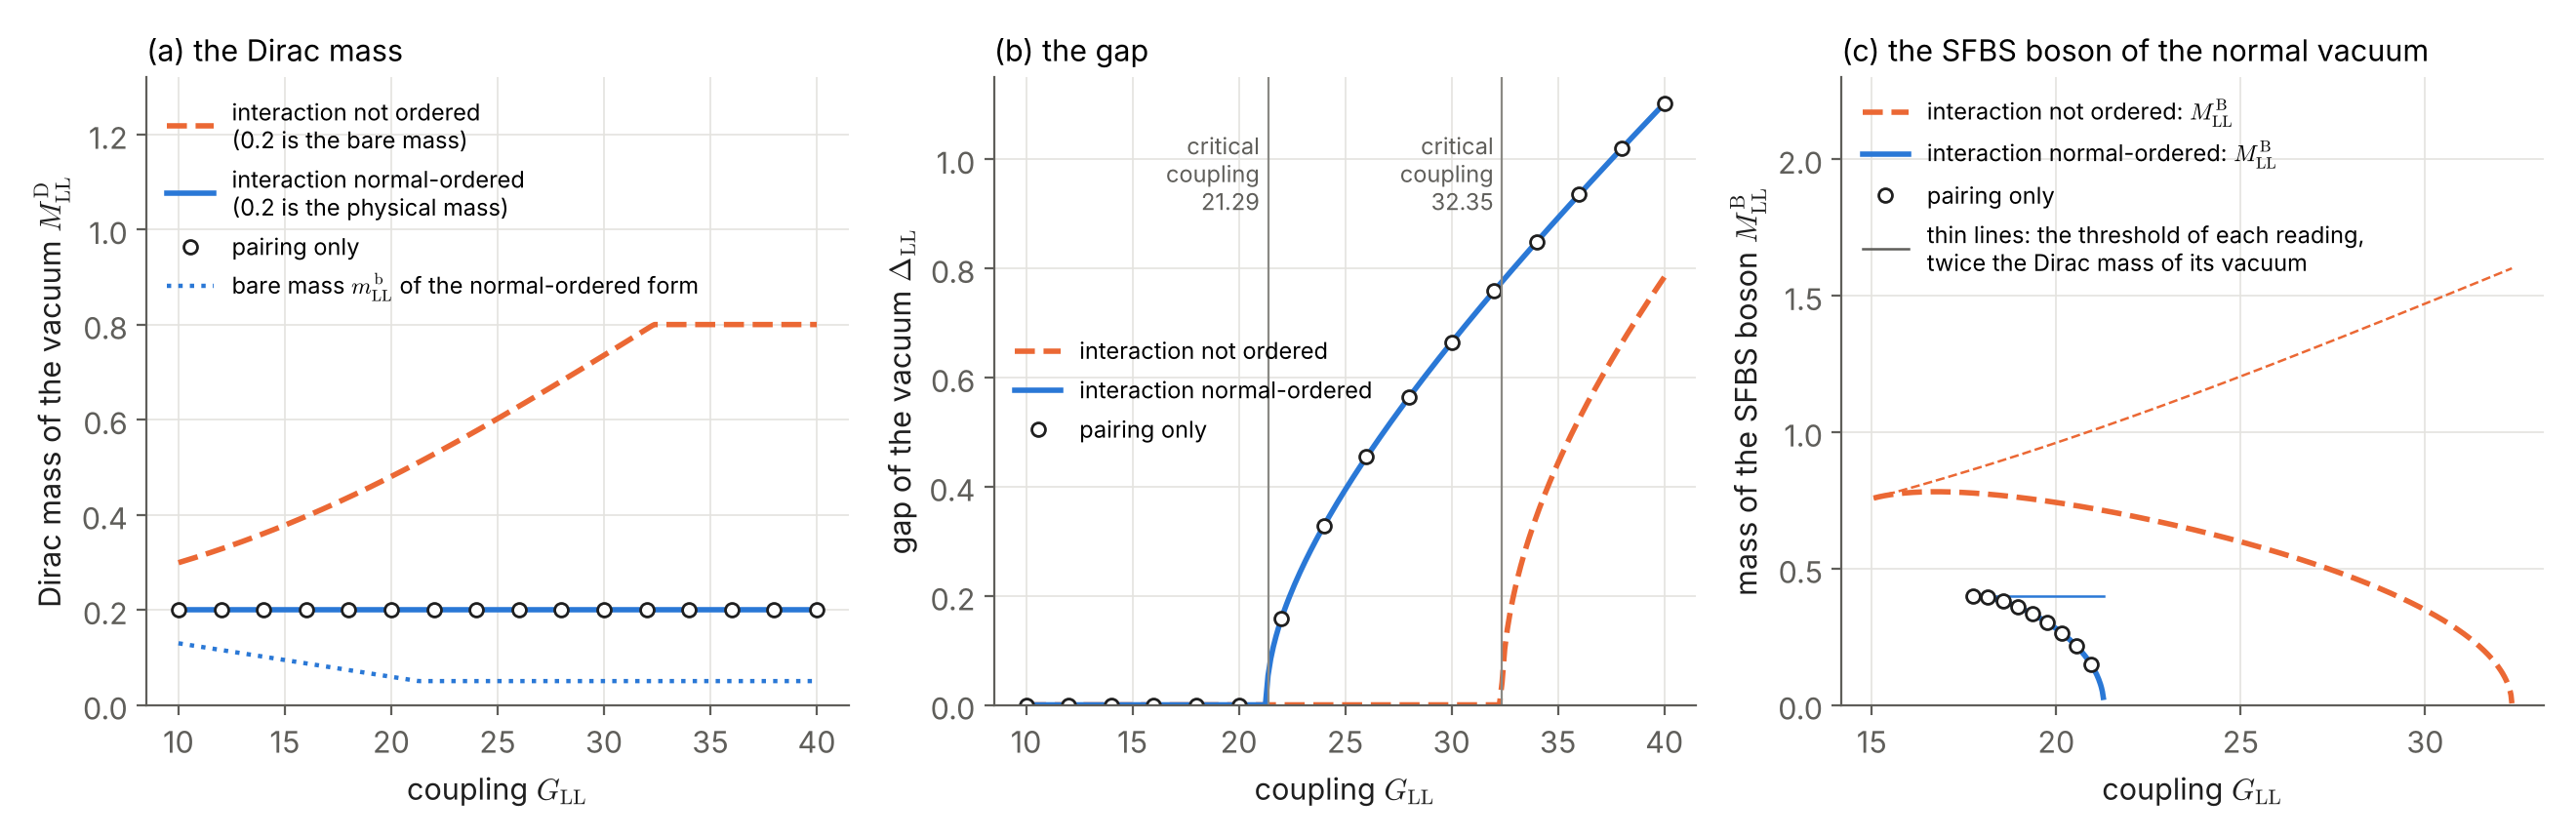
\includegraphics[width=1\textwidth,height=\textheight]{figures/fig_t2_cjt_vacuum.png}

\textbf{Figure 1.} The vacuum against the coupling \(G_{\rm LL}\) for
the mass 0.2 (\(\Lambda_{\rm LL}=1\)). Dashed: the interaction not
ordered (0.2 is the bare mass). Solid: the interaction normal-ordered
(0.2 is the mass of the spinor charges). Circles: the pairing-only
treatment of the document of Test 2. (a) The Dirac mass of the vacuum;
the dotted curve is the bare mass (7.6) of the normal-ordered form. (b)
The gap; the vertical lines mark the two critical couplings. (c) The
mass of the SFBS boson of the normal vacuum (Section 8.1), thick curves,
and the threshold of two spinor charges, thin curves. The solid curves
and the circles coincide: the normal-ordered two-loop vacuum and its
boson are those of the pairing-only treatment.

\hypertarget{what-the-pairing-only-treatment-is-and-what-remains-different}{%
\subsection{7.3 What the pairing-only treatment is, and what remains
different}\label{what-the-pairing-only-treatment-is-and-what-remains-different}}

The pairing-only treatment is the functional without the normal term,
\[\mathcal E^{\rm po}_{\rm LL}=\mathcal E^{\rm no}_{\rm LL}+\tfrac12G_{\rm LL}\sum_\iota\mathrm{tr}\big(\mathsf K^\iota_{\rm LL}(\mathsf C^{\rm n}_{\rm LL}-\mathsf C^{\rm vac}_{\rm LL})(\mathsf K^\iota_{\rm LL})^\dagger(\mathsf C^{\rm n}_{\rm LL}-\mathsf C^{\rm vac}_{\rm LL})^T\big).\tag{7.7}\]
The two functionals have the same value and the same first derivatives
at the vacuum, hence the same vacuum and the same gap equation. They
differ in the second order of
\(\mathsf C^{\rm n}_{\rm LL}-\mathsf C^{\rm vac}_{\rm LL}\), by (4.2) in
every channel with its own coefficient. Three consequences:

\begin{itemize}
\tightlist
\item
  \textbf{States far from the vacuum are dressed.} Above the critical
  coupling the normal stationary state is not the state with the Dirac
  mass \(m_{\rm LL}\): by (6.6) with the bare mass (7.6) it has
  \(M^{\rm N}_{\rm LL}=0.227347\) at \(G_{\rm LL}=22.5\). The condensed
  vacuum lies 3.8816e-5 below it (in units \(\Lambda_{\rm LL}^4\)); the
  pairing-only treatment, whose normal state keeps the mass 0.2, gives
  5.2884e-5. Figure 2 shows the energy (6.4) of the trial states: at
  \(G_{\rm LL}=20\) a single minimum, the normal vacuum; at
  \(G_{\rm LL}=22.5\) the minimum at the gap 0.2094933 and the normal
  stationary state as a saddle, displaced to the larger Dirac mass.
\item
  \textbf{The oscillations about the condensed vacuum mix pair and
  normal channels.} In a condensed vacuum the fermion number is not
  conserved, and a change of the gap changes the scalar density. The
  masses of the massive oscillations therefore differ from those of the
  pairing-only treatment. They are derived in stages G and H.
\item
  \textbf{The normal vacuum is not affected}: there the pair channel is
  separated from all normal channels by the conservation of the fermion
  number (Theorem D7).
\end{itemize}

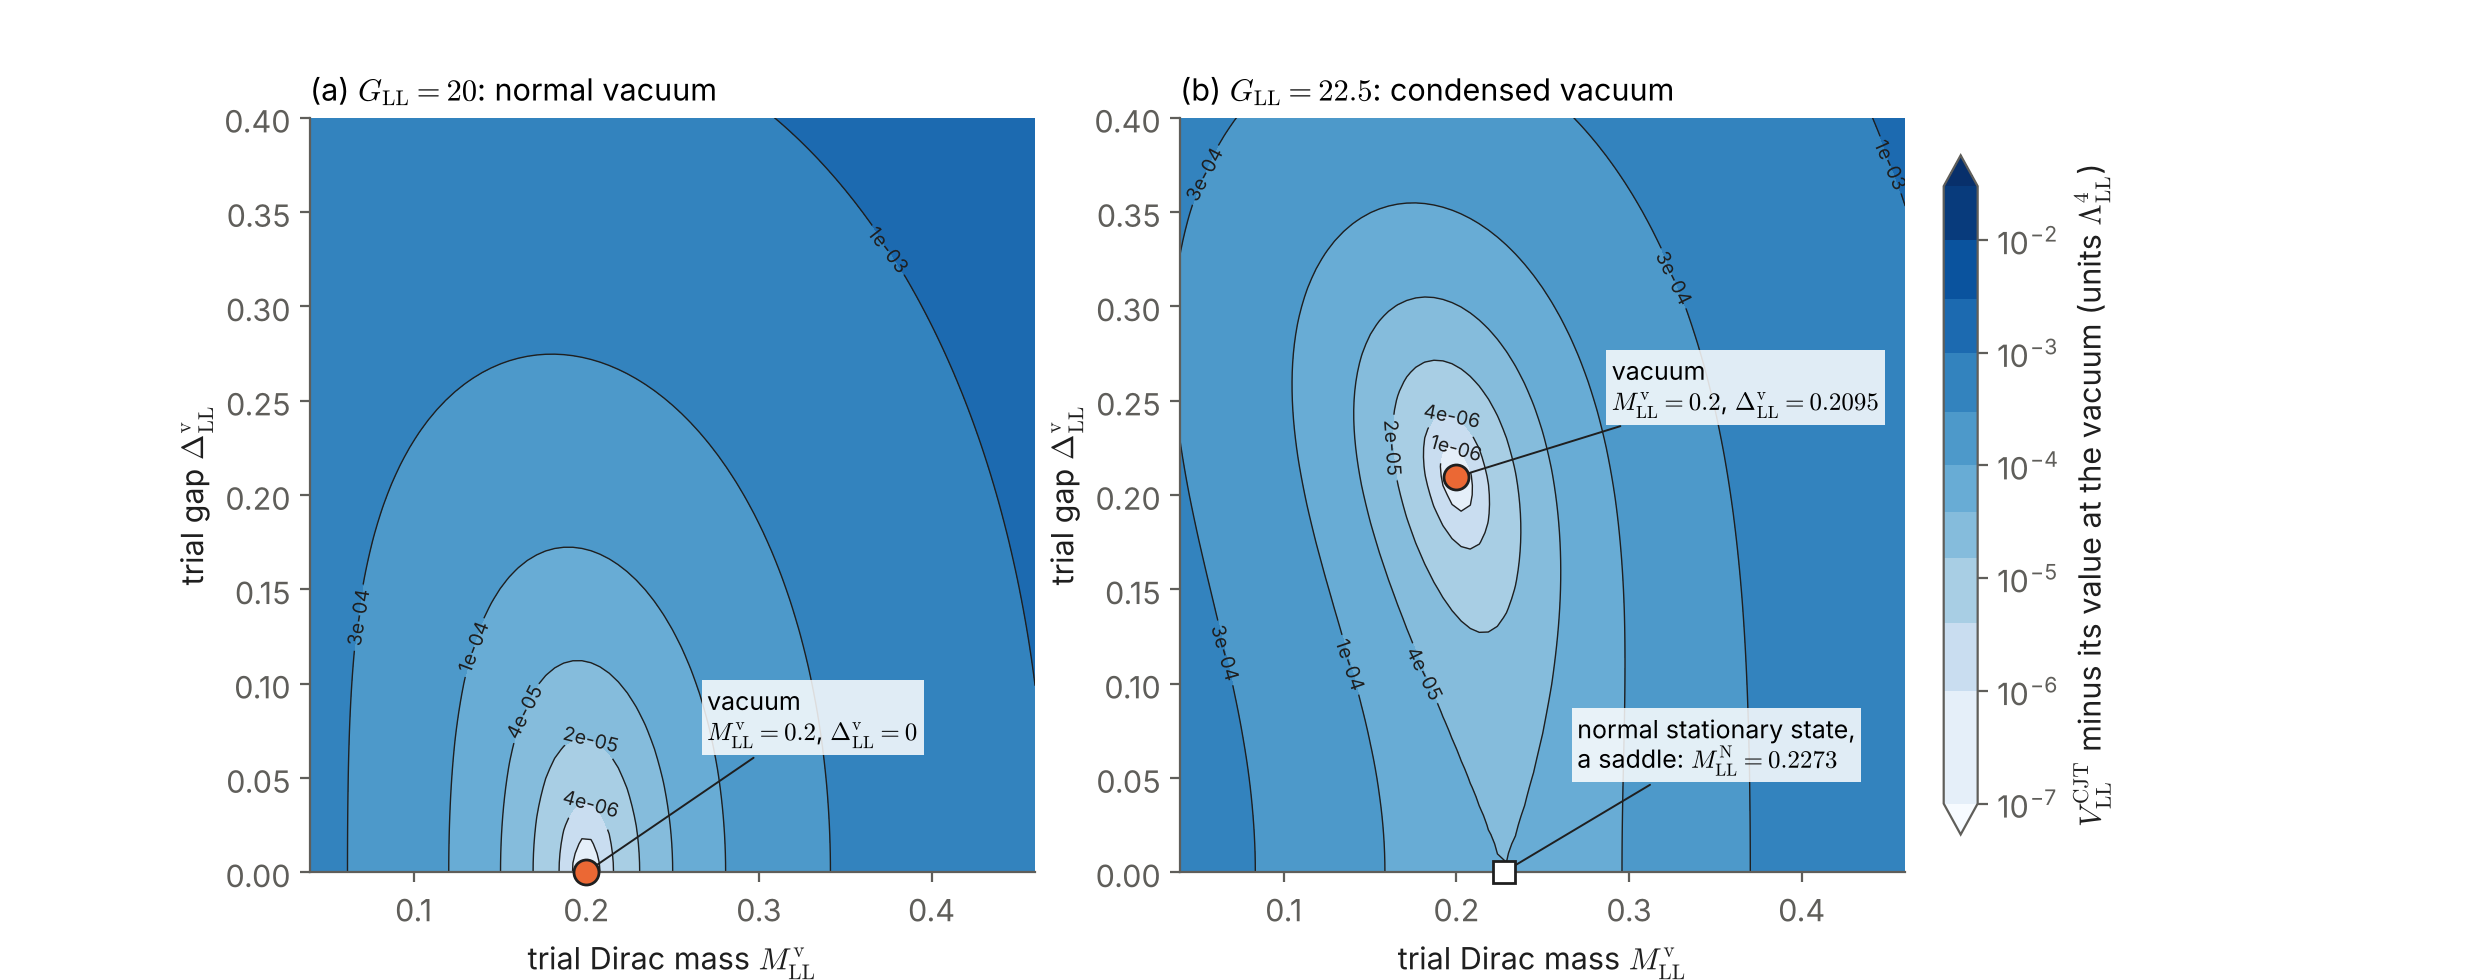
\includegraphics[width=1\textwidth,height=\textheight]{figures/fig_t2_cjt_surface.png}

\textbf{Figure 2.} The two-loop energy per volume (6.4) of the trial
states of the vacuum sector, minus its value at the vacuum, against the
trial Dirac mass and the trial gap, for \(m_{\rm LL}=0.2\) in the
normal-ordered form (contour lines at the values written on them; darker
is higher). (a) \(G_{\rm LL}=20\), below the critical coupling: the
vacuum is the normal state. (b) \(G_{\rm LL}=22.5\): the vacuum (filled
circle) is condensed; the normal stationary state (open square) is a
saddle, 3.8816e-5 above the vacuum (data file
\texttt{test2/data/t2\_cjt\_surface.csv}).

\hypertarget{an-alternative-that-changes-the-interaction}{%
\subsection{7.4 An alternative that changes the
interaction}\label{an-alternative-that-changes-the-interaction}}

A second way to remove the dressing of the mass changes the model
instead of its reading. The chirality rotation by a quarter turn,
\(\Psi_{\rm LL}\mapsto\exp(\tfrac14i\pi\gamma^{\rm ch}_{\rm LL})\Psi_{\rm LL}\),
turns every scalar pair operator into \(i\) times a pseudoscalar one,
\(\Pi^\iota_{\rm LL}\mapsto i\,\Pi'^\iota_{\rm LL}\) and
\(\Pi'^\iota_{\rm LL}\mapsto i\,\Pi^\iota_{\rm LL}\), where
\(\Pi'^\iota_{\rm LL}=\Psi^T_{\rm LL}\mathsf K'^\iota_{\rm LL}\Psi_{\rm LL}\)
with
\(\mathsf K'^\iota_{\rm LL}=C_{\rm LL}\otimes\mathsf E_{\rm LL}\tau^{\rm LL}_\iota\);
a chirality rotation by another angle mixes the two, with the cosine and
\(i\) times the sine of twice the angle as coefficients. The interaction
of (2.4) is not invariant under these rotations; the sum
\[\tfrac14G_{\rm LL}\sum_\iota\big((\Pi^\iota_{\rm LL})^\dagger\Pi^\iota_{\rm LL}+(\Pi'^\iota_{\rm LL})^\dagger\Pi'^\iota_{\rm LL}\big)\tag{7.8}\]
is, and only the mass term then breaks this symmetry.

\textbf{Theorem D8 (the axially symmetric completion).} For the
interaction (7.8): (a) the coefficients of the normal channels are the
sums \(c^A_{\rm LL}+c'^A_{\rm LL}\) of Table 1, which vanish for the
four classes of channels that change the chirality (\(\beta_{\rm LL}\),
\(i\beta_{\rm LL}\gamma^{\rm ch}_{\rm LL}\),
\(i\beta_{\rm LL}\alpha^j_{\rm LL}\),
\(\beta_{\rm LL}\gamma^{\rm ch}_{\rm LL}\alpha^j_{\rm LL}\)); (b) hence
no state dresses the Dirac mass:
\(M^{\rm D}_{\rm LL}=m^{\rm b}_{\rm LL}\) always, and no counterterm for
the mass is needed; (c) the shift of the chemical potential is
\(3G_{\rm LL}N^\Lambda_{\rm LL}\) instead of
\(\tfrac32G_{\rm LL}N^\Lambda_{\rm LL}\); (d) the state (7.4) with
\(m^{\rm b}_{\rm LL}=m_{\rm LL}\) is a stationary state, with vanishing
pseudoscalar pair amplitudes.

\emph{Proof.} (a) and (c) are Theorems D3 and D4 for the two sets of
pair matrices together (the pseudoscalar pair matrices are antisymmetric
and unitary as well, so that (5.1) holds for them). (b) follows from
(4.3). (d): the correlation matrices (6.3) give no pseudoscalar
amplitude because
\(\mathrm{tr}(\mathsf K'^\iota_{\rm LL}(\mathsf K^3_{\rm LL})^\dagger)=0\),
and the conditions (6.5) hold with the coefficient of the first one
replaced by zero. \(\blacksquare\)

\emph{Check CJ-11} verifies (a) to (d) numerically, and finds from a
random start with scalar and pseudoscalar pair fields the state (7.4)
again (pseudoscalar amplitude below \(10^{-12}\)).

This alternative is \textbf{not adopted}: it is a different interaction
from the one the author specified, it has a second, pseudoscalar, pair
channel, and its oscillations would have to be worked out anew. It is
recorded because it is the form in which the pairing-only treatment of
the vacuum and of its Dirac mass is exact at two loops for every state.
The choice between the two is the author's.

\hypertarget{why-the-normal-contractions-cannot-be-removed-for-all-states}{%
\subsection{7.5 Why the normal contractions cannot be removed for all
states}\label{why-the-normal-contractions-cannot-be-removed-for-all-states}}

One may ask for an interaction whose normal contractions vanish in every
state, so that the pairing-only treatment would be the whole two-loop
result. There is none. A general interaction of two particles at a point
is
\(\tfrac14\sum\mathsf V_{aba'b'}\Psi^\dagger_{{\rm LL},a}\Psi^\dagger_{{\rm LL},b}\Psi_{{\rm LL},b'}\Psi_{{\rm LL},a'}\)
with coefficients \(\mathsf V_{aba'b'}\) (a letter used in this section
only) that are antisymmetric in the first two and in the last two
indices. Its normal contraction is
\(\tfrac12\sum\mathsf V_{aba'b'}(\mathsf C^{\rm n}_{\rm LL})_{a'a}(\mathsf C^{\rm n}_{\rm LL})_{b'b}\),
a quadratic form in \(\mathsf C^{\rm n}_{\rm LL}\) whose coefficients
are already symmetric under the exchange of the two factors. It vanishes
for all Hermitian matrices only if all \(\mathsf V_{aba'b'}\) vanish.
The normal contractions can be subtracted at one state, the vacuum, and
no more; Definition 7.1 does exactly that.

\hypertarget{the-creation-of-the-sfbs}{%
\section{8. The creation of the SFBS}\label{the-creation-of-the-sfbs}}

\hypertarget{the-sfbs-boson-a-pole-of-the-pair-part-of-the-propagator}{%
\subsection{8.1 The SFBS boson: a pole of the pair part of the
propagator}\label{the-sfbs-boson-a-pole-of-the-pair-part-of-the-propagator}}

\emph{The equations of motion.} The stationarity condition of the
two-loop action for a propagator that depends on the time is the
time-dependent form of Theorem D2 (b): with
\((\mathcal G^{\rm fr}_{\rm LL})^{-1}=i\partial_0-\) (the free matrix),
the self-energy stays a matrix (3.9) at one time, and the density matrix
of the Nambu spinor obeys
\[i\,\partial_0\mathsf R^{\rm Nb}_{\rm LL}(\vec q_{\rm LL})=\big[\mathsf H^{\rm var}_{\rm LL}(\vec q_{\rm LL}),\mathsf R^{\rm Nb}_{\rm LL}(\vec q_{\rm LL})\big],\tag{8.1}\]
with the mean fields (3.9) of the state at that time (the time-dependent
Hartree-Fock-Bogoliubov equations). Equivalently every occupied vector
of \(\mathsf R^{\rm Nb}_{\rm LL}\) obeys
\(i\partial_0(\text{vector})=\mathsf H^{\rm var}_{\rm LL}(\text{vector})\).
The energy is conserved: by the proof of Theorem D2 (b),
\(\partial_0\mathcal E^{\rm var}_{\rm LL}=\tfrac12\int\mathrm{tr}(\mathsf H^{\rm var}_{\rm LL}\partial_0\mathsf R^{\rm Nb}_{\rm LL}) =-\tfrac i2\int\mathrm{tr}(\mathsf H^{\rm var}_{\rm LL}[\mathsf H^{\rm var}_{\rm LL},\mathsf R^{\rm Nb}_{\rm LL}])=0\).

\emph{The pair susceptibility.} In the normal-ordered form the normal
vacuum has the Dirac mass \(m_{\rm LL}\), and a spinor charge of the
momentum \(\vec q_{\rm LL}\) has the energy
\(\varepsilon_{\rm LL}=(q_{\rm LL}^2+m_{\rm LL}^2)^{1/2}\). For a
frequency \(\omega^{\rm B}_{\rm LL}\) of the pair field at the wave
number zero let
\[\chi^{\rm pr}_{\rm LL}(\omega^{\rm B}_{\rm LL},0)=\int_{q_{\rm LL}<\Lambda_{\rm LL}}\frac{d^3q_{\rm LL}}{(2\pi)^3}\frac{8\varepsilon_{\rm LL}}{4\varepsilon_{\rm LL}^2-(\omega^{\rm B}_{\rm LL})^2}.\tag{8.2}\]
Below the threshold \(2m_{\rm LL}\) of two spinor charges the integral
is, in closed form,
\[\begin{aligned}\pi^2\chi^{\rm pr}_{\rm LL}(\omega^{\rm B}_{\rm LL},0)={}&\tfrac12\Big(\Lambda_{\rm LL}\varepsilon_{\rm LL}(\Lambda_{\rm LL})+m_{\rm LL}^2\,\mathrm{arsinh}\frac{\Lambda_{\rm LL}}{m_{\rm LL}}\Big)
-\Big(m_{\rm LL}^2-\tfrac14(\omega^{\rm B}_{\rm LL})^2\Big)\mathrm{arsinh}\frac{\Lambda_{\rm LL}}{m_{\rm LL}}\\
&-\tfrac12\omega^{\rm B}_{\rm LL}\Big(m_{\rm LL}^2-\tfrac14(\omega^{\rm B}_{\rm LL})^2\Big)^{1/2}\arctan\frac{\Lambda_{\rm LL}\,\omega^{\rm B}_{\rm LL}}{2\varepsilon_{\rm LL}(\Lambda_{\rm LL})\big(m_{\rm LL}^2-\tfrac14(\omega^{\rm B}_{\rm LL})^2\big)^{1/2}},\end{aligned}\tag{8.3}\]
where
\(\varepsilon_{\rm LL}(\Lambda_{\rm LL})=(\Lambda_{\rm LL}^2+m_{\rm LL}^2)^{1/2}\).
For an imaginary frequency
\(\omega^{\rm B}_{\rm LL}=i\gamma^{\rm gr}_{\rm LL}\) the second line is
replaced by
\(+\tfrac12\gamma^{\rm gr}_{\rm LL}\big(m_{\rm LL}^2+\tfrac14(\gamma^{\rm gr}_{\rm LL})^2\big)^{1/2}\)
times the inverse hyperbolic tangent of
\(\Lambda_{\rm LL}\gamma^{\rm gr}_{\rm LL}/\big(2\varepsilon_{\rm LL}(\Lambda_{\rm LL})(m_{\rm LL}^2+\tfrac14(\gamma^{\rm gr}_{\rm LL})^2)^{1/2}\big)\).
As a function of \((\omega^{\rm B}_{\rm LL})^2\) on the real line below
\(4m_{\rm LL}^2\), (8.2) increases: from 0 at minus infinity, through
its value at zero frequency, to its value at the threshold,
\[\begin{aligned}\chi^{\rm pr}_{\rm LL}(0,0)&=2\,\Xi^{(1)}_{\rm LL}(m_{\rm LL}^2)=\frac1{G^{\rm crit}_{\rm LL}},\\
\chi^{\rm pr}_{\rm LL}(2m_{\rm LL},0)&=\frac1{2\pi^2}\Big(\Lambda_{\rm LL}\varepsilon_{\rm LL}(\Lambda_{\rm LL})+m_{\rm LL}^2\,\mathrm{arsinh}\frac{\Lambda_{\rm LL}}{m_{\rm LL}}\Big)=\frac1{G^{\rm bd}_{\rm LL}}\end{aligned}\tag{8.4}\]
The second equation defines the \textbf{binding coupling}
\(G^{\rm bd}_{\rm LL}\); the first is the critical coupling (7.5). For a
normal state with another Dirac mass (the vacuum of the interaction that
is not ordered, or the normal stationary state above the critical
coupling, both with \(M^{\rm N}_{\rm LL}\) of (6.6)) that mass stands in
the place of \(m_{\rm LL}\) in (8.2) to (8.4).

\textbf{Theorem D7 (the SFBS boson).} Let the vacuum be normal. A small
oscillation of the pair field about it,
\(d^\iota_{\rm LL}\propto\exp(-i\omega^{\rm B}_{\rm LL}x^0_{\rm LL})\)
at the wave number zero, is a solution of the linearized equations (8.1)
exactly when
\[G_{\rm LL}\,\chi^{\rm pr}_{\rm LL}(\omega^{\rm B}_{\rm LL},0)=1,\tag{8.5}\]
for each of the three components \(\iota\) separately, and to the first
order it changes no normal mean field. Hence: (a) for
\(G_{\rm LL}<G^{\rm bd}_{\rm LL}\) there is no oscillation below the
threshold: two spinor charges do not bind; (b) for
\(G^{\rm bd}_{\rm LL}<G_{\rm LL}<G^{\rm crit}_{\rm LL}\) there is
exactly one, with a real frequency \(M^{\rm B}_{\rm LL}\) between 0 and
\(2m_{\rm LL}\): \textbf{a boson of spin 0 made of two spinor charges,
the SFBS boson}, with the binding energy
\(2m_{\rm LL}-M^{\rm B}_{\rm LL}\). It is a complex isospin vector:
three components with the fermion number \(+2\) and their three
antiparticles; (c) \(M^{\rm B}_{\rm LL}\) decreases from \(2m_{\rm LL}\)
at \(G^{\rm bd}_{\rm LL}\) to 0 at \(G^{\rm crit}_{\rm LL}\); (d) for
\(G_{\rm LL}>G^{\rm crit}_{\rm LL}\) the root is imaginary,
\(\omega^{\rm B}_{\rm LL}=i\gamma^{\rm gr}_{\rm LL}\): the pair field
grows as \(\exp(\gamma^{\rm gr}_{\rm LL}x^0_{\rm LL})\), the normal
state is unstable, and the SFBS condenses.

\emph{Proof.} In this proof \(\mathsf h_{\rm LL}\) is the matrix (2.5)
with the Dirac mass \(m_{\rm LL}\) of the vacuum, so that
\((\mathsf h_{\rm LL})^2=\varepsilon_{\rm LL}^2\). In the normal vacuum
the matrix (3.6) is block diagonal, with the blocks
\(\mathsf h_{\rm LL}(\vec q_{\rm LL})\) and
\(-\mathsf h_{\rm LL}(-\vec q_{\rm LL})^T\), and by the proof of Theorem
D5
\(\mathsf C^{\rm n}_{\rm LL}(\vec q_{\rm LL})=\tfrac12(1-\mathsf h_{\rm LL}/\varepsilon_{\rm LL})\)
and \(\mathsf C^{\rm p}_{\rm LL}(\vec q_{\rm LL})=0\). Add a small
pairing block
\(\mathsf P_{\rm LL}=\sum_\iota d^\iota_{\rm LL}(\mathsf K^\iota_{\rm LL})^\dagger\).
To the first order a pair correlation matrix
\(\mathsf C^{\rm p}_{\rm LL}(\vec q_{\rm LL})\) appears, and nothing
else: a fermion-number transformation multiplies the pairing block and
the pair correlation matrix by a phase and leaves the normal correlation
matrix unchanged, so that the normal correlation matrix, and with it
every normal mean field, changes in the second order only. By (3.7) the
upper right block of (8.1) is an equation for
\(\mathsf C^{\rm p}_{\rm LL}\),
\[i\partial_0\mathsf C^{\rm p}_{\rm LL}(\vec q_{\rm LL})=\mathsf h_{\rm LL}(\vec q_{\rm LL})\,\mathsf C^{\rm p}_{\rm LL}(\vec q_{\rm LL})+\mathsf C^{\rm p}_{\rm LL}(\vec q_{\rm LL})\,\mathsf h_{\rm LL}(-\vec q_{\rm LL})^T
-\mathsf P_{\rm LL}\big(1-\mathsf C^{\rm n}_{\rm LL}(-\vec q_{\rm LL})^T\big)+\mathsf C^{\rm n}_{\rm LL}(\vec q_{\rm LL})\,\mathsf P_{\rm LL}.\tag{8.6}\]
The identity
\(\mathsf h_{\rm LL}(\vec q_{\rm LL})(\mathsf K^\iota_{\rm LL})^\dagger=(\mathsf K^\iota_{\rm LL})^\dagger\mathsf h_{\rm LL}(-\vec q_{\rm LL})^T\)
(proof of Theorem D5; it holds for each \(\iota\)) turns the last two
terms into
\(-\sum_\iota d^\iota_{\rm LL}(\mathsf h_{\rm LL}/\varepsilon_{\rm LL})(\mathsf K^\iota_{\rm LL})^\dagger\).
The ansatz
\[\mathsf C^{\rm p}_{\rm LL}(\vec q_{\rm LL})=-\sum_\iota\Big(u^{{\rm pr},\iota}_{\rm LL}+w^{{\rm pr},\iota}_{\rm LL}\,\frac{\mathsf h_{\rm LL}(\vec q_{\rm LL})}{\varepsilon_{\rm LL}}\Big)(\mathsf K^\iota_{\rm LL})^\dagger\tag{8.7}\]
with two functions \(u^{{\rm pr},\iota}_{\rm LL}\),
\(w^{{\rm pr},\iota}_{\rm LL}\) of the length of the momentum and of the
time for every component closes the equation, by the same identity:
\[i\partial_0u^{{\rm pr},\iota}_{\rm LL}=2\varepsilon_{\rm LL}w^{{\rm pr},\iota}_{\rm LL},\qquad
i\partial_0w^{{\rm pr},\iota}_{\rm LL}=2\varepsilon_{\rm LL}u^{{\rm pr},\iota}_{\rm LL}+d^\iota_{\rm LL}.\tag{8.8}\]
For the time dependence \(\exp(-i\omega^{\rm B}_{\rm LL}x^0_{\rm LL})\)
this gives
\(u^{{\rm pr},\iota}_{\rm LL}=2\varepsilon_{\rm LL}d^\iota_{\rm LL}/((\omega^{\rm B}_{\rm LL})^2-4\varepsilon_{\rm LL}^2)\).
By (3.5) and (8.7) the pair amplitude is
\(\langle\Pi^\iota_{\rm LL}\rangle=8\int_{q_{\rm LL}<\Lambda_{\rm LL}}d^3q_{\rm LL}(2\pi)^{-3}u^{{\rm pr},\iota}_{\rm LL}=-2d^\iota_{\rm LL}\chi^{\rm pr}_{\rm LL}\)
(the term with \(w^{{\rm pr},\iota}_{\rm LL}\) has no trace), and the
self-consistency
\(d^\iota_{\rm LL}=-\tfrac12G_{\rm LL}\langle\Pi^\iota_{\rm LL}\rangle\)
is (8.5). (a) to (d) follow from the monotony of (8.2) in
\((\omega^{\rm B}_{\rm LL})^2\) and from (8.4). The spin is 0 and the
isospin 1 by Section 2.1. \(\blacksquare\)

\emph{Check CJ-7} computes the response of the six real pair operators
and of the 64 normal operators to pair fields from the eigenvectors of
the \(16\times16\) matrices at three frequencies: the pair-pair response
is \(-2\chi^{\rm pr}_{\rm LL}\) times the unit matrix, with (8.3)
reproduced to \(10^{-15}\), and the response of every normal operator
vanishes; (8.3) agrees with a quadrature of (8.2), also at an imaginary
frequency; the root of (8.5) tends to \(2m_{\rm LL}\) at
\(G^{\rm bd}_{\rm LL}\) and to 0 at \(G^{\rm crit}_{\rm LL}\).

For the mass 0.2 in the normal-ordered form:
\(G^{\rm bd}_{\rm LL}=17.7463\) and \(G^{\rm crit}_{\rm LL}=21.28661\).
Table 4 gives the boson mass between them; Figure 1 (c) shows it. These
are the values of the pairing-only treatment, because (8.5) contains the
Dirac mass of the vacuum and nothing else. Without the normal ordering
the same theorem holds with the Dirac mass \(M^{\rm N}_{\rm LL}\) of
(6.6), which depends on the coupling, in the place of \(m_{\rm LL}\);
the boson is then bound from 15.036 up to 32.3506 (dashed in Figure 1
(c)).

\sptkeptpenalty=10000
\begin{longtable}[]{@{}
  >{\raggedright\arraybackslash}p{(\columnwidth - 4\tabcolsep) * \real{0.2593}}
  >{\raggedright\arraybackslash}p{(\columnwidth - 4\tabcolsep) * \real{0.3704}}
  >{\raggedright\arraybackslash}p{(\columnwidth - 4\tabcolsep) * \real{0.3704}}@{}}
\toprule\noalign{}
\begin{minipage}[b]{\linewidth}\raggedright
\(G_{\rm LL}\)
\end{minipage} & \begin{minipage}[b]{\linewidth}\raggedright
\(M^{\rm B}_{\rm LL}\)
\end{minipage} & \begin{minipage}[b]{\linewidth}\raggedright
\(2m_{\rm LL}-M^{\rm B}_{\rm LL}\)
\end{minipage} \\
\midrule\noalign{}
\endhead
\bottomrule\noalign{}
\endlastfoot
18 & 0.397362 & 0.002638 \\*
19 & 0.356465 & 0.043535 \\*
20 & 0.279252 & 0.120748 \\*
20.5 & 0.221990 & 0.178010 \\*
21 & 0.135923 & 0.264077 \\*
21.2 & 0.075108 & 0.324892 \\
\end{longtable}

\textbf{Table 4.} The mass of the SFBS boson of the normal vacuum, and
its binding energy, for \(m_{\rm LL}=0.2\) in the normal-ordered form
(data file \texttt{test2/data/t2\_cjt\_boson.csv}).

\hypertarget{the-creation-in-real-time}{%
\subsection{8.2 The creation in real
time}\label{the-creation-in-real-time}}

The statements of Theorem D7 are statements about the linearized
equations. The full equations (8.1) were integrated in time to see the
SFBS appear. \emph{The integration:} the occupied vectors of every
momentum (8 vectors of 16 components for each of 128 momenta along one
axis; this is exact for states that are covariant under rotations: the
16 Dirac matrices are scalars and vectors under rotations, so that the
correlation matrices of such a state are polynomials of the first degree
in the direction of the momentum, and two opposite directions average
them exactly) obey
\(i\partial_0(\text{vector})=\mathsf H^{\rm var}_{\rm LL}(\text{vector})\)
with the mean fields (3.9) of the current state; the integrator is CVODE
of the library SUNDIALS (Adams-Moulton formulas of variable order and
step, relative tolerance \(10^{-13}\), absolute tolerance \(10^{-15}\));
it took 14481 and 5823 internal steps for the two runs. \emph{The
initial states:} the ground state of the mean-field matrix of a normal
stationary state to which the small pair seed
\(\epsilon^{\rm sd}_{\rm LL}(\mathsf K^3_{\rm LL})^\dagger\) is added.
Both runs use \(m_{\rm LL}=0.2\) in the normal-ordered form.

\textbf{Run 1: \(G_{\rm LL}=20\), between the binding and the critical
coupling; \(\epsilon^{\rm sd}_{\rm LL}=10^{-4}\).} The pair amplitude
\(\langle\Pi^3_{\rm LL}\rangle\) stays real and oscillates without
damping (Figure 3 (a)). The frequency of the largest line of its
spectrum (Hann window over the 600 time units of the run) is 0.279252;
the root of (8.5) is \(M^{\rm B}_{\rm LL}=0.279252\); the relative
difference is 1.0e-7. The Dirac mass does not move (change below
\(10^{-8}\), of the second order in the seed): the SFBS boson rings
alone.

\textbf{Run 2: \(G_{\rm LL}=22.5\), above the critical coupling;
\(\epsilon^{\rm sd}_{\rm LL}=10^{-8}\).} The start is the normal
stationary state (Dirac mass 0.227347). The modulus of the pair
amplitude grows exponentially over five orders of magnitude (Figure 3
(b)). The rate fitted on that stretch is 0.249607; the root of (8.5) at
an imaginary frequency, with the Dirac mass of this state in (8.2), is
\(\gamma^{\rm gr}_{\rm LL}=0.249608\); the relative difference is
6.2e-7. The growth ends when the amplitude reaches the size of that of
the condensed vacuum,
\(2\Delta^{\rm vac}_{\rm LL}/G_{\rm LL}=0.018622\): it overshoots to
0.025354 and then oscillates about a mean of 0.013341, with a swing that
decreases slowly. It does not come to rest in the vacuum, and it cannot:
the equations (8.1) conserve the energy, the initial state lies above
the vacuum by the depth of Section 7.3, and that energy stays in the
oscillation and in the excited spinor charges. To reach the vacuum the
energy must be carried away, by the graphs beyond two loops or by a
coupling to other fields. In both runs the energy was conserved to
better than \(10^{-10}\).

\emph{Check CJ-8} contains both runs and these comparisons.

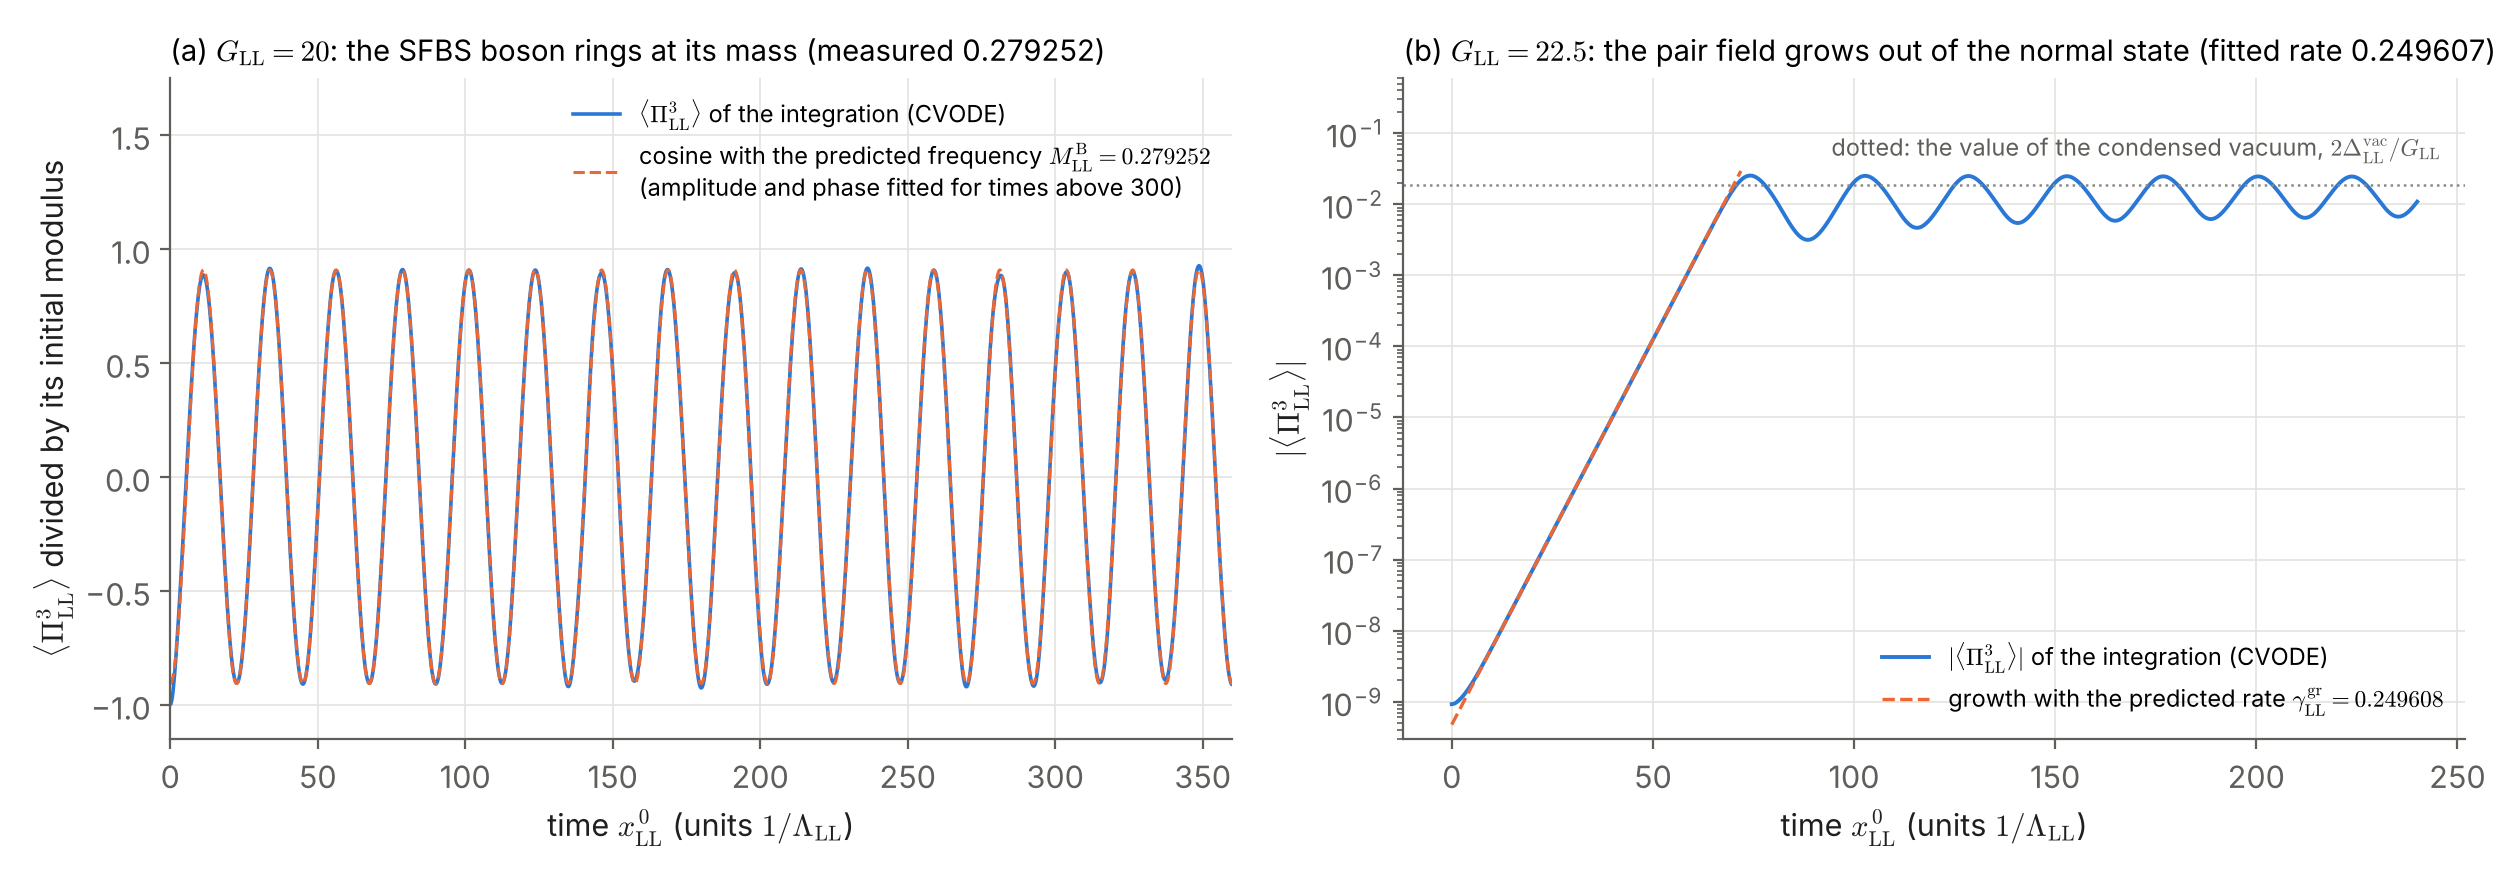
\includegraphics[width=1\textwidth,height=\textheight]{figures/fig_t2_cjt_creation.png}

\textbf{Figure 3.} The creation of the SFBS in real time, from the
integration of the time-dependent equations (8.1) of the two-loop action
by CVODE (\(m_{\rm LL}=0.2\), normal-ordered form). (a)
\(G_{\rm LL}=20\): the pair amplitude of the normal vacuum after a small
seed (solid), and a cosine with the predicted frequency
\(M^{\rm B}_{\rm LL}\) of (8.5) whose amplitude and phase are fitted at
late times (dashed); the two curves coincide. (b) \(G_{\rm LL}=22.5\):
the modulus of the pair amplitude on a logarithmic scale (solid), the
exponential with the predicted rate \(\gamma^{\rm gr}_{\rm LL}\)
(dashed), and the value of the condensed vacuum (dotted) (data file
\texttt{test2/data/t2\_cjt\_time.csv}).

\hypertarget{the-creation-of-the-sfbs-in-the-language-of-the-method}{%
\subsection{8.3 The creation of the SFBS, in the language of the
method}\label{the-creation-of-the-sfbs-in-the-language-of-the-method}}

\begin{enumerate}
\def\labelenumi{\arabic{enumi}.}
\tightlist
\item
  \emph{The operator.} The SFBS is the pair part of the propagator of
  the Nambu spinor at coinciding points,
  \(\langle\Pi^\iota_{\rm LL}\rangle\) of (3.5), a Lorentz scalar and an
  isospin vector with the fermion number 2; its field is the order
  parameter (2.7), which enters the method as the pair part
  \(\mathsf P_{\rm LL}\) of the self-energy (3.9). Nothing is added to
  the theory of the spinor field: the boson field is a part of its
  propagator.
\item
  \emph{The particle.} The second derivative of the two-loop action at
  the normal vacuum, in the direction of the pair part, vanishes at the
  frequency \(M^{\rm B}_{\rm LL}\) of (8.5): the pair part of the
  propagator has a pole there, below the threshold of two spinor
  charges, for couplings between \(G^{\rm bd}_{\rm LL}\) and
  \(G^{\rm crit}_{\rm LL}\). The interaction has created a boson out of
  two spinor charges.
\item
  \emph{The condensate.} At \(G^{\rm crit}_{\rm LL}\) the mass of the
  boson is zero. Above, the stationary propagator with the lowest energy
  has a pair part: the gap equation (7.4), a vacuum with
  \(\vec d_{\rm LL}\ne0\) that breaks \(U(1)^{\rm F}_{\rm LL}\) and
  \(SU(2)_{\rm v}\). The normal state decays into it with the rate
  \(\gamma^{\rm gr}_{\rm LL}\). This vacuum is the superfluid, and the
  oscillations of its order parameter are the subject of stages E to I.
\end{enumerate}

\hypertarget{discussion}{%
\section{9. Discussion}\label{discussion}}

\hypertarget{how-good-is-the-two-loop-approximation}{%
\subsection{9.1 How good is the two-loop
approximation?}\label{how-good-is-the-two-loop-approximation}}

Theorem D2 (c) bounds the exact ground energy from above; it does not
say how close the bound is. A test in which the exact answer is known is
one site: the 8 modes of Theorem D4 with the Hamiltonian
\(\sum_{k,k'}\hat c^\dagger_{{\rm LL},k}(m^{\rm b}_{\rm LL}\beta_{\rm LL}\otimes\mathsf 1_2-\mu^{\rm b}_{\rm LL})_{kk'}\hat c_{{\rm LL},k'}-\tfrac14G_{\rm LL}\sum_\iota(\hat\Pi^\iota_{\rm LL})^\dagger\hat\Pi^\iota_{\rm LL}\)
at \(\mu^{\rm b}_{\rm LL}=-\tfrac32G_{\rm LL}\), whose 256 eigenvalues
are found by diagonalization; its lowest one is \(E^{\rm ex}_{\rm LL}\).
Table 5 and Figure 4 compare it with the lowest two-loop energy.

\sptkeptpenalty=10000
\begin{longtable}[]{@{}
  >{\raggedright\arraybackslash}p{(\columnwidth - 8\tabcolsep) * \real{0.1200}}
  >{\raggedright\arraybackslash}p{(\columnwidth - 8\tabcolsep) * \real{0.2200}}
  >{\raggedright\arraybackslash}p{(\columnwidth - 8\tabcolsep) * \real{0.2200}}
  >{\raggedright\arraybackslash}p{(\columnwidth - 8\tabcolsep) * \real{0.2200}}
  >{\raggedright\arraybackslash}p{(\columnwidth - 8\tabcolsep) * \real{0.2200}}@{}}
\toprule\noalign{}
\begin{minipage}[b]{\linewidth}\raggedright
\(G_{\rm LL}\)
\end{minipage} & \begin{minipage}[b]{\linewidth}\raggedright
exact ground energy \(E^{\rm ex}_{\rm LL}\)
\end{minipage} & \begin{minipage}[b]{\linewidth}\raggedright
two-loop energy \(\mathcal E^{\rm var}_{\rm LL}\)
\end{minipage} & \begin{minipage}[b]{\linewidth}\raggedright
difference
\end{minipage} & \begin{minipage}[b]{\linewidth}\raggedright
\(\lvert\vec d_{\rm LL}\rvert\) of the two-loop state
\end{minipage} \\
\midrule\noalign{}
\endhead
\bottomrule\noalign{}
\endlastfoot
0.1 & -0.914847 & -0.800000 & 0.114847 & 0.000000 \\*
0.2 & -1.163806 & -0.800000 & 0.363806 & 0.000000 \\*
0.3 & -1.474923 & -0.800000 & 0.674923 & 0.000000 \\*
0.5 & -2.180214 & -0.820000 & 1.360214 & 0.600000 \\*
0.75 & -3.124245 & -0.963333 & 2.160912 & 1.268858 \\*
1 & -4.094372 & -1.160000 & 2.934372 & 1.833030 \\*
1.5 & -6.063508 & -1.606667 & 4.456841 & 2.891366 \\*
2 & -8.047791 & -2.080000 & 5.967791 & 3.919184 \\*
3 & -12.031938 & -3.053333 & 8.978604 & 5.946427 \\*
4 & -16.023974 & -4.040000 & 11.983974 & 7.959899 \\
\end{longtable}

\textbf{Table 5.} One site (8 fermion modes, bare mass 0.2,
charge-symmetric chemical potential): the exact ground energy, the
lowest two-loop energy found (three starts), their difference, and the
modulus of the order parameter of the two-loop state (data file
\texttt{test2/data/t2\_cjt\_site.csv}).

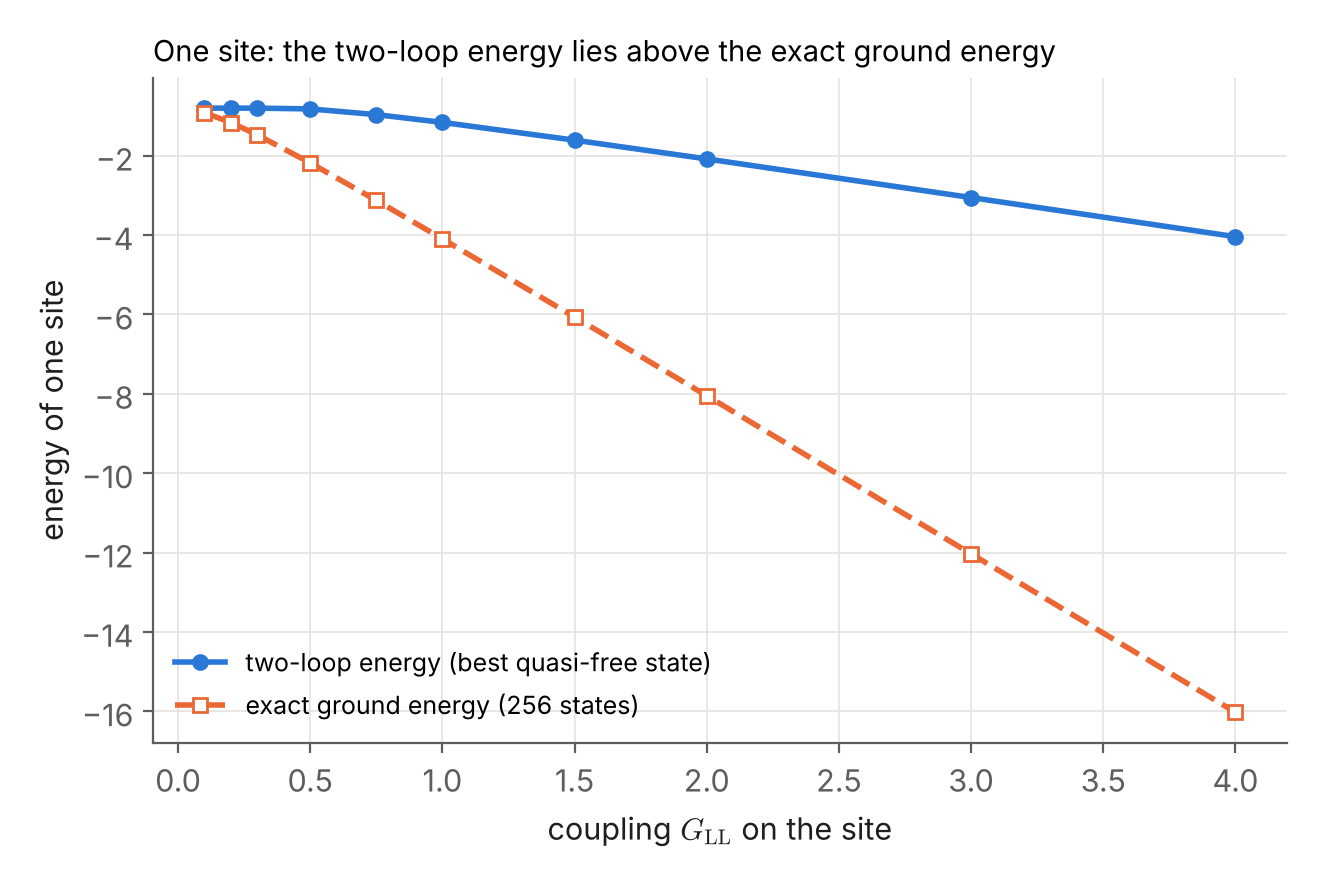
\includegraphics[width=0.62\textwidth,height=\textheight]{figures/fig_t2_cjt_site.png}

\textbf{Figure 4.} One site: the two-loop energy (solid, circles) and
the exact ground energy (dashed, squares) against the coupling.

Two things are verified (check CJ-10): the two-loop energy is the
expectation value of the Hamiltonian in the mean-field state constructed
explicitly in the Fock space (difference below \(10^{-14}\)), and it is
never below the exact ground energy. A third thing is seen: on one site
the bound is poor. This is expected and is not a statement about the
field theory. A single site has no continuum of momenta: its order
parameter is not a classical variable, the exact ground state is a
superposition of all its directions and phases (a state of definite
fermion number and isospin), and this superposition gains an energy that
no quasi-free state has. In the field theory the same fluctuations
exist; they are the graphs of three and more loops of Section 3.3, the
exchange of the SFBS boson. Their size relative to two loops is not
estimated in this document. The two-loop results of this document are
the mean-field theory of the model, exact in its own terms and verified
as such, and the corrections to them are open.

\hypertarget{the-earlier-treatment-and-this-one-side-by-side}{%
\subsection{9.2 The earlier treatment and this one, side by
side}\label{the-earlier-treatment-and-this-one-side-by-side}}

\sptkeptpenalty=10000
\begin{longtable}[]{@{}
  >{\raggedright\arraybackslash}p{(\columnwidth - 6\tabcolsep) * \real{0.2987}}
  >{\raggedright\arraybackslash}p{(\columnwidth - 6\tabcolsep) * \real{0.2338}}
  >{\raggedright\arraybackslash}p{(\columnwidth - 6\tabcolsep) * \real{0.2338}}
  >{\raggedright\arraybackslash}p{(\columnwidth - 6\tabcolsep) * \real{0.2338}}@{}}
\toprule\noalign{}
\begin{minipage}[b]{\linewidth}\raggedright
Statement
\end{minipage} & \begin{minipage}[b]{\linewidth}\raggedright
Pairing only (the document of Test 2)
\end{minipage} & \begin{minipage}[b]{\linewidth}\raggedright
Two loops, not ordered
\end{minipage} & \begin{minipage}[b]{\linewidth}\raggedright
Two loops, normal-ordered
\end{minipage} \\
\midrule\noalign{}
\endhead
\bottomrule\noalign{}
\endlastfoot
contractions of the interaction kept & pair-pair & all three & all
three; the normal ones of the vacuum subtracted \\*
chemical potential of the vacuum & 0 &
\(\mu^{\rm b}_{\rm LL}=-\tfrac32G_{\rm LL}N^\Lambda_{\rm LL}\) &
\(\mu_{\rm LL}=0\) \\*
Dirac mass of the vacuum for the mass 0.2 & 0.2 & 0.539206 at
\(G_{\rm LL}=22.5\); 0.8 if condensed & 0.2 \\*
critical coupling & 21.28661 & 32.3506 & 21.28661 \\*
vacuum at \(G_{\rm LL}=22.5\) & condensed, gap 0.2094933 & normal &
condensed, gap 0.2094933 \\*
binding coupling & 17.7463 & 15.036 & 17.7463 \\*
boson mass at \(G_{\rm LL}=20\) & 0.279252 & 0.741755 (Dirac mass
0.4803) & 0.279252 \\*
normal stationary state at \(G_{\rm LL}=22.5\) & Dirac mass 0.2 & Dirac
mass 0.539206 (the vacuum) & Dirac mass 0.227347 \\*
energy of the condensed vacuum at \(G_{\rm LL}=22.5\), measured from the
normal stationary state & -5.2884e-5 & none & -3.8816e-5 \\*
a variational bound on the energy & no & yes & yes \\
\end{longtable}

\textbf{Table 6.} The three treatments. The first and the third column
agree in everything that concerns the vacuum and the normal vacuum's
boson; they differ in the last three rows.

The last row deserves a remark. The pairing-only functional (7.7) is not
the expectation value of a Hamiltonian in its trial states, by Section
7.5; it is not a bound. The two-loop functional is. This is the sense in
which the method of CJT is the more complete treatment: it is the same
calculation with the terms restored that make it a variational
principle.

\hypertarget{what-is-decided-here-and-what-is-the-authors-to-decide}{%
\subsection{9.3 What is decided here, and what is the author's to
decide}\label{what-is-decided-here-and-what-is-the-authors-to-decide}}

Decided here, because one reading had to be chosen to continue: the
parameters \(m_{\rm LL}\), \(\mu_{\rm LL}\), \(G_{\rm LL}\) of Test 2
are read in the normal-ordered form of Section 7.1. All numbers of Test
2 for the vacuum then stand as they are. The author's to decide: whether
to prefer the alternative of Section 7.4, which changes the interaction;
and whether the differences of Section 7.3 at the second order (the
dressed normal state, the masses of the oscillations of the condensed
vacuum) are to be kept, as the method of CJT requires and as stages E to
I will do unless told otherwise, or to be suppressed for the sake of
agreement with the earlier treatment, which would be the pairing-only
functional (7.7) under another name.

\hypertarget{appendix-a.-provenance}{%
\section{Appendix A. Provenance}\label{appendix-a.-provenance}}

\hypertarget{a.1-how-to-reproduce-everything}{%
\subsection{A.1 How to reproduce
everything}\label{a.1-how-to-reproduce-everything}}

From the folder Revision\_SuperLoop of the repository:

\begin{verbatim}
# 1. the checks CJ-1 to CJ-11, the numbers and tables of this document, the data of its figures (about one minute)
(cd test2/rust && cargo build --release) && ./test2/rust/target/release/t2_cjt
# 2. Figures 1 to 4 (test2/figures/fig_t2_cjt_*.pdf and .png)
python3 test2/python/make_t2_cjt_figures.py
# 3. everything of the folder Revision_SuperLoop, all checks and all documents, with one verdict ("ALL PASS")
bash code/scripts/check_all.sh
\end{verbatim}

Requirements: a Rust toolchain (edition 2021); Python 3 with NumPy and
Matplotlib for the figures. No crate is downloaded: the program uses the
library \texttt{t2core} of the workspace and, through it, the
translation of SUNDIALS 7.8.0 into pure Rust that is kept in the folder
\texttt{vendor/sundials\_rs-7.8.0} of the project (the integrator
CVODE).

\hypertarget{a.2-the-program}{%
\subsection{A.2 The program}\label{a.2-the-program}}

\texttt{test2/rust/t2cjt/src/main.rs} (binary \texttt{t2\_cjt}, a member
of the Cargo workspace \texttt{test2/rust}) is one commented source
file. It reuses two modules of the member \texttt{t2sfbs} of the same
workspace: \texttt{fock.rs}, the Fock space of a few fermion modes
(operators applied to vectors of \(2^8\) components), and
\texttt{quad.rs}, Gauss-Legendre quadrature. Its parts:

\begin{itemize}
\tightlist
\item
  \emph{the model}: the pair matrices, the matrix
  \(\mathsf h_{\rm LL}\), the mean fields (3.9), the two interaction
  terms of (3.8); the momentum grids (a product rule in the length, the
  polar angle and the azimuth; the two directions of one axis; one
  site);
\item
  \emph{the state}: for every momentum of a grid the matrix (3.6) is
  diagonalized (Householder reduction and the QL iteration of
  \texttt{t2core}), and the correlation matrices (3.4) are summed from
  the eigenvectors with negative eigenvalues, by (3.7);
\item
  \emph{the self-consistency}: the map from mean fields to the mean
  fields of their ground state, iterated with Anderson acceleration
  (depth 6, damping 0.6) until the residual is below \(10^{-12}\);
\item
  \emph{the closed forms}: (6.2), (6.4), the roots of (6.6), (6.8),
  (7.4) and (8.5) by bisection (200 halvings), and (8.3);
\item
  \emph{the time integration}: the right side of (8.1) for the occupied
  vectors, given to CVODE through the interface \texttt{t2core::cvode};
  the frequency of run 1 by the maximum of a Hann-windowed Fourier sum
  (scan, then golden-section search), the rate of run 2 by a
  least-squares line through the logarithm of the modulus;
\item
  \emph{the checks} CJ-1 to CJ-11, each a function of the program, with
  the report below.
\end{itemize}

The figures are drawn by \texttt{test2/python/make\_t2\_cjt\_figures.py}
from the data files; that script computes nothing except the fit of the
dashed cosine of Figure 3 (a).

\hypertarget{a.3-the-report-of-the-checks}{%
\subsection{A.3 The report of the
checks}\label{a.3-the-report-of-the-checks}}

The file \texttt{test2/data/t2\_cjt\_checks.txt}, as the program wrote
it. The names in it are the plain-text names of the symbols (Appendix
C): for example \texttt{C\_n}, \texttt{C\_p} for the correlation
matrices, \texttt{N\_sc} for the normal mean field, \texttt{E\_var} for
the functional (3.8), \texttt{V\_CJT} for (6.4), \texttt{M\_trial},
\texttt{Delta\_trial} for the trial parameters, \texttt{m\_bare},
\texttt{mu\_bare} for the bare parameters, \texttt{Kch\_iota} for the
pair matrices and \texttt{Pi\_iota} for the pair operators.

\begin{Shaded}
\begin{Highlighting}[]
\NormalTok{Revision\_SuperLoop, folder test2, program \textasciigrave{}t2\_cjt\textasciigrave{}: the creation of the superfluid boson singlet state (SFBS) from the spinor field Psi\_LL by the method of Cornwall, Jackiw and Tomboulis, in the two{-}loop approximation of the effective action of the propagator (Test 2, stage D)}
\NormalTok{11 of 11 checks passed}

\NormalTok{[PASS] CJ{-}1  Wick\textquotesingle{}s theorem for the interaction, in the Fock space of one site (8 fermion modes, 256 states): for the ground state of a random quadratic Hamiltonian c\^{}dag h c + (1/2)(c\^{}dag P c\^{}dag\^{}T + Hermitian conjugate) (h Hermitian, P antisymmetric, both random), \textless{}sum\_iota Pi\_iota\^{}dag Pi\_iota\textgreater{} computed directly in the Fock space equals sum\_iota |\textless{}Pi\_iota\textgreater{}|\^{}2 + 2 sum\_iota tr(Kch\_iota C\_n Kch\_iota\^{}dag C\_n\^{}T); and the correlation matrices C\_n[a][b] = \textless{}c\_b\^{}dag c\_a\textgreater{}, C\_p[a][b] = \textless{}c\_a c\_b\textgreater{} of that ground state are the upper left block and minus the upper right block of the projector on the eigenvectors with negative eigenvalues of the matrix [[h, P], [P\^{}dag, {-}h\^{}T]] of 16 rows  {-}{-} 4 random Hamiltonians: largest |direct {-} Wick| = 9.4e{-}14; largest difference of C\_n 2.0e{-}14, of C\_p 1.7e{-}14 between the Fock space and the matrix of 16 rows; smallest gap above the ground state 0.001}
\NormalTok{[PASS] CJ{-}2  the 64 normal channels: for every matrix T = D (x) tau\_b (D one of the 16 Hermitian Dirac matrices 1, beta, i beta gamma\_ch, gamma\_ch, alpha\^{}j, gamma\_ch alpha\^{}j, i beta alpha\^{}j, beta gamma\_ch alpha\^{}j; tau\_0 the unit matrix), sum\_iota Kch\_iota T Kch\_iota\^{}dag = c\_ch T\^{}T with c\_ch = sign\_D times 3 for tau\_0 and sign\_D times 1 for tau\_iota, sign\_D = +1 for 1, beta, gamma\_ch, i beta alpha\^{}j and {-}1 for the other four classes; the same for the pseudoscalar pair matrices Kch\textquotesingle{}\_iota with the signs +1 for 1, i beta gamma\_ch, gamma\_ch, beta gamma\_ch alpha\^{}j and {-}1 for the other four; the 64 matrices are Hermitian with tr(T\_ch T\_ch\textquotesingle{}) = 8 or 0; and for a random Hermitian C\_n the mean field N\_sc = {-}G sum\_iota Kch\_iota\^{}dag C\_n\^{}T Kch\_iota equals {-}(G/8) sum\_ch c\_ch n\_ch T\_ch and the normal term of the energy equals {-}(G/16) sum\_ch c\_ch n\_ch\^{}2, with n\_ch = tr(T\_ch C\_n)  {-}{-} largest entry of sum K T K\^{}dag {-} c\_ch T\^{}T 0.0e0; largest |c\_ch {-} expected| 0.0e0; orthogonality 0.0e0; mean field 3.4e{-}16; normal energy 4.4e{-}16}
\NormalTok{[PASS] CJ{-}3  the order of the factors of the interaction and the charge conjugation, on one site (256 states): sum\_iota [Pi\_iota, Pi\_iota\^{}dag] = 48 {-} 12 n\_F\_site for the scalar pair operators and for the pseudoscalar ones (n\_F\_site: the number of spinor charges on the site); there is a matrix U\_C = D (x) tau\_b with U\_C\^{}dag alpha\^{}j U\_C = (alpha\^{}j)\^{}T, U\_C\^{}dag beta U\_C = {-}beta\^{}T, for which {-}(U\_C\^{}T Kch\_iota U\_C)\^{}* is a unitary combination of the Kch\_iota (the exchange c\_a {-}\textgreater{} sum\_b U\_C[a][b] c\_b\^{}dag of particles and holes keeps the kinetic term and turns sum Pi\^{}dag Pi into sum Pi Pi\^{}dag); and the 256 eigenvalues of the Hamiltonian of one site with the chemical potential mu equal those with the chemical potential {-}mu {-} 3 G, shifted by {-}8 mu {-} 12 G  {-}{-} commutator: largest entry of the difference 0.0e0 (scalar), 0.0e0 (pseudoscalar); U\_C = (i beta alpha\^{}2) (x) tau\_0 (largest violation 0.0e0); spectra: largest difference 6.4e{-}14 for (m, mu, G) = (0.191, 0.505, 1.569), (m, mu, G) = (0.421, {-}0.624, 0.978), (m, mu, G) = (0.488, 0.022, 0.794)}
\NormalTok{[PASS] CJ{-}4  the terms of the effective action on the trial family: (a) for the spectra e\_k, e\textquotesingle{}\_k of two random particle{-}hole symmetric Hermitian matrices of 16 rows, (1/4) int dw/(2 pi) sum\_k ln((w\^{}2 + e\_k\^{}2)/(w\^{}2 + e\textquotesingle{}\_k\^{}2)) = (1/4) sum\_k (|e\_k| {-} |e\textquotesingle{}\_k|) (the trace{-}log term is minus the ground energy of the trial Hamiltonian), the spectrum is symmetric about zero, and {-}(1/2) sum\_k sign(e\_k) v\_k v\_k\^{}dag = R\_Nb {-} 1/2 with R\_Nb the projector on the negative eigenvalues (the symmetric equal{-}time limit of the propagator); (b) for trial states of the vacuum sector with the Dirac mass M\_trial and the gap Delta\_trial (bare mass 0.05, G = 22.5, charge{-}symmetric chemical potential), the energy E\_var from the matrices of 16 rows on the momentum grid equals the closed form V\_CJT = {-}2 Xi + 4 (M\_trial {-} m\_bare) s\_c + 4 Delta\_trial f\_c {-} 3 G s\_c\^{}2 {-} 4 G f\_c\^{}2 + 3 G N\_Lambda\^{}2, with C\_n = (N\_Lambda/2) {-} (s\_c/2) beta and \textless{}Pi\_3\textgreater{} = {-}4 f\_c, \textless{}Pi\_1\textgreater{} = \textless{}Pi\_2\textgreater{} = 0; and the gradient of V\_CJT is (4 (M\_trial {-} m\_bare) {-} 6 G s\_c) grad s\_c + (4 Delta\_trial {-} 8 G f\_c) grad f\_c  {-}{-} (a) frequency integral 0.7041280531 against 0.7041280531 (difference 2.1e{-}11); symmetry of the spectrum 1.6e{-}15; equal{-}time limit 5.4e{-}16; (b) 4 trial states: largest |E\_var {-} V\_CJT| 3.2e{-}15, C\_n 7.6e{-}17, \textless{}Pi\textgreater{} 3.8e{-}17, gradient against central differences 1.8e{-}12}
\NormalTok{[PASS] CJ{-}5  the stationary states of the vacuum sector with bare parameters, at the charge{-}symmetric chemical potential mu\_bare = {-}(3/2) G N\_Lambda: the normal state with the Dirac mass M\_N, the root of M\_N = m\_bare + (3/2) G M\_N Xi\_1(M\_N\^{}2), and, above the critical coupling G\_crit\_bare = 1/(2 Xi\_1(16 m\_bare\^{}2)), the condensed state with the Dirac mass M\_D = 4 m\_bare exactly and the gap from 1 = 2 G Xi\_1(16 m\_bare\^{}2 + Delta\^{}2), are fixed points of the general self{-}consistency map of the matrices of 16 rows (mean fields reproduced); both have the density 4 N\_Lambda (half filling); their energies equal the closed form V\_CJT; the condensed state lies below the normal one where it exists, M\_N \textgreater{} 4 m\_bare there and M\_N \textless{} 4 m\_bare below the critical coupling; and M\_N = 4 m\_bare at the critical coupling (the transition is continuous)  {-}{-} largest residual of the mean fields 5.1e{-}15; density {-} 4 N\_Lambda 5.8e{-}16; |M\_D {-} 4 m\_bare| 5.6e{-}16; |E\_var {-} V\_CJT| 3.2e{-}15; |M\_N(G\_crit\_bare) {-} 4 m\_bare| 0.0e0; (m\_bare, G) = (0.05, 18): normal M\_N = 0.1442960, no condensed state; (m\_bare, G) = (0.05, 22.5): normal M\_N = 0.2273467, condensed M\_D = 4 m\_bare = 0.2, gap 0.2094933, E\_c {-} E\_n = {-}3.8816e{-}5; (m\_bare, G) = (0.05, 30): normal M\_N = 0.4566355, condensed M\_D = 4 m\_bare = 0.2, gap 0.6641406, E\_c {-} E\_n = {-}1.4993e{-}3; (m\_bare, G) = (0.2, 15): normal M\_N = 0.3779745, no condensed state; (m\_bare, G) = (0.2, 22.5): normal M\_N = 0.5392059, no condensed state; (m\_bare, G) = (0.2, 40): normal M\_N = 1.0135753, condensed M\_D = 4 m\_bare = 0.8, gap 0.7839054, E\_c {-} E\_n = {-}5.7262e{-}4}
\NormalTok{[PASS] CJ{-}6  the normal ordering of the interaction with respect to the vacuum, at the parameters of the document of Test 2 (m = 0.2, G = 22.5, Lambda = 1): (a) the state with the Dirac mass M\_D = m and the gap of the pairing{-}only gap equation 1 = 2 G Xi\_1(m\^{}2 + Delta\^{}2) is a stationary state of the functional with the bare parameters m\_bare = m {-} (3/2) G s\_vac = m/4 and mu\_bare = {-}(3/2) G N\_Lambda; (b) for random states the normal{-}ordered functional E\_no, in which C\_n {-} C\_vac replaces C\_n in the normal term and m, mu = 0 replace m\_bare, mu\_bare, differs from the bare functional E\_var by the same constant, the normal term of the vacuum; (c) the critical coupling 1/(2 Xi\_1(m\^{}2)) = 21.28661 and the gap Delta\_vac = 0.2094933 of the pairing{-}only theory are reproduced; (d) without the normal ordering (0.2 as bare mass) the vacuum at G = 22.5 is normal, with the Dirac mass M\_N = 0.539206, and the critical coupling is 1/(2 Xi\_1(16 m\^{}2)) = 32.35; (e) on a grid of 81 x 81 trial states (M\_trial from 0.04 to 0.46, Delta\_trial from 0 to 0.4) no energy lies below that of the vacuum  {-}{-} (a) residual of the mean fields 2.4e{-}15; |m\_bare {-} (m {-} (3/2) G s\_vac)| 1.4e{-}17; m\_bare = 0.0500000; (b) largest deviation from the constant 1.7e{-}16 (constant {-}0.0205820501); (c) G\_crit = 21.2866098, Delta\_vac = 0.2094933; (d) M\_N = 0.5392059, G\_crit\_bare = 32.3505912; (e) smallest V\_CJT {-} V\_CJT(vacuum) on the grid 7.3e{-}8}
\NormalTok{[PASS] CJ{-}7  the SFBS boson of the normal vacuum (m = 0.2, G = 20, interaction normal{-}ordered; momentum grid along the axis): the response of the pair operators (Pi\_iota + Pi\_iota\^{}dag)/2 and (Pi\_iota {-} Pi\_iota\^{}dag)/(2 i) to fields coupled to the same six operators, computed from the eigenvectors of the matrices of 16 rows at the frequencies 0, 0.25 and 0.39, is {-}2 chi\_pr times the unit matrix, with chi\_pr = int 8 eps/(4 eps\^{}2 {-} omega\_B\^{}2) in its closed form; the response of the 64 normal operators Psi\_LL\^{}dag T\_ch Psi\_LL to these fields vanishes (no mixing in the normal vacuum); the closed form of chi\_pr agrees with a quadrature, also at an imaginary frequency; chi\_pr(0) = 2 Xi\_1(m\^{}2) = 1/G\_crit; the pole condition G chi\_pr(M\_B\^{}2) = 1 has a root below the threshold 2 m, which tends to 2 m at the binding coupling G\_bind and to 0 at the critical coupling  {-}{-} largest deviation of the diagonal from {-}2 chi\_pr 3.1e{-}16; other pair entries 2.5e{-}18; mixing with the normal channels 0.0e0; closed form against quadrature 2.8e{-}17; M\_B(G = 20) = 0.2792516 with |G chi\_pr {-} 1| = 0.0e0; G\_bind = 17.7462765, G\_crit = 21.2866098; M\_B just above G\_bind 0.4000000, just below G\_crit 3.7e{-}5}
\NormalTok{[PASS] CJ{-}8  the creation of the SFBS in real time: the time{-}dependent mean{-}field equations of the two{-}loop action, i dv/dt = H\_var(q) v for the occupied vectors of every momentum with the mean fields of the current state, integrated by CVODE (Adams{-}Moulton formulas, rtol 1e{-}13, atol 1e{-}15; m = 0.2, interaction normal{-}ordered, 128 momenta along the axis). Run 1, G = 20 (between G\_bind and G\_crit), start: the normal vacuum with the pair seed 1e{-}4 Kch\_3\^{}dag in its mean{-}field matrix: \textless{}Pi\_3\textgreater{} stays real and oscillates, and the frequency of the largest line of its Hann{-}windowed Fourier sum equals the boson mass M\_B of the pole condition; the Dirac mass stays at m to the second order in the seed. Run 2, G = 22.5 (above G\_crit), start: the normal stationary state with the seed 1e{-}8: |\textless{}Pi\_3\textgreater{}| grows exponentially with the rate gamma\_gr, the root of G chi\_pr({-}gamma\_gr\^{}2) = 1 for the Dirac mass of that state; the growth ends in oscillations about the condensed vacuum, in which |\textless{}Pi\_3\textgreater{}| reaches between one half and twice the value 2 Delta\_vac/G of the condensed vacuum (the equations conserve the energy, so that the state cannot come to rest in the vacuum). Both integrations conserve the energy E\_var to better than 1e{-}9  {-}{-} run 1: frequency 0.2792516 against M\_B = 0.2792516 (relative difference 1.0e{-}7); largest |Im \textless{}Pi\_3\textgreater{}| 2.5e{-}12; largest |Dirac mass {-} m| 8.8e{-}9; change of the energy 6.2e{-}11; 14481 steps, 28956 evaluations of the right side. Run 2: fitted rate 0.2496075 over 186 output times against gamma\_gr = 0.2496077 (relative difference 6.2e{-}7); largest |\textless{}Pi\_3\textgreater{}| 0.0253535 and mean over the last third 0.0133409 against 2 Delta\_vac/G = 0.0186216; change of the energy 2.8e{-}11; 5823 steps, 11640 evaluations}
\NormalTok{[PASS] CJ{-}9  general solutions of the two{-}loop equations without imposed symmetry (m = 0.2, G = 22.5, interaction normal{-}ordered; 384 momenta in a product grid): from four random starts (random Hermitian N\_sc, random complex order parameter) the Anderson iteration of the self{-}consistency map of the full matrices of 16 rows converges; no solution has an energy below that of the vacuum of the closed form; and the solutions that reach this energy have |dvec| = Delta\_vac, zeta = 0 and the Dirac mass m (they are the vacuum (0, 0, Delta\_vac) turned by a symmetry transformation)  {-}{-} start 1: 36 iterations, residual 1.2e{-}12, E {-} E\_vacuum = {-}6.661e{-}16, |d| = 0.2094933, zeta = 1.1e{-}10, M\_D = 0.2000000 (the condensed vacuum); start 2: 51 iterations, residual 1.0e{-}12, E {-} E\_vacuum = {-}8.674e{-}16, |d| = 0.2094933, zeta = 4.6e{-}11, M\_D = 0.2000000 (the condensed vacuum); start 3: 40 iterations, residual 8.7e{-}13, E {-} E\_vacuum = {-}8.327e{-}17, |d| = 0.2094933, zeta = 6.5e{-}11, M\_D = 0.2000000 (the condensed vacuum); start 4: 39 iterations, residual 5.6e{-}13, E {-} E\_vacuum = 0.000e0, |d| = 0.2094933, zeta = 3.2e{-}11, M\_D = 0.2000000 (the condensed vacuum)}
\NormalTok{[PASS] CJ{-}10  the two{-}loop action is a variational energy, tested on one site (8 fermion modes, 256 states; m = 0.2, chemical potential {-}(3/2) G, ten couplings from 0.1 to 4): the energy E\_var of the self{-}consistent mean{-}field state equals the expectation value of the Hamiltonian c\^{}dag (m beta {-} mu) c {-} (G/4) sum\_iota Pi\_iota\^{}dag Pi\_iota in the ground state of the mean{-}field Hamiltonian, constructed in the Fock space; and it is never below the exact ground energy (the lowest eigenvalue of the 256 x 256 matrix)  {-}{-} largest |E\_var {-} expectation value| 5.1e{-}15; smallest E\_var {-} exact ground energy 0.114847; largest residual of the mean fields 9.0e{-}14}
\NormalTok{[PASS] CJ{-}11  the alternative without mass dressing, the axially symmetric completion {-}(G/4) sum\_iota (Pi\_iota\^{}dag Pi\_iota + Pi\textquotesingle{}\_iota\^{}dag Pi\textquotesingle{}\_iota) of the interaction (pseudoscalar pair operators Pi\textquotesingle{}\_iota of the matrices Kch\textquotesingle{}\_iota): the sums of the coefficients of the scalar and of the pseudoscalar pairs vanish on the four classes of channels that flip the chirality (beta, i beta gamma\_ch, i beta alpha\^{}j, beta gamma\_ch alpha\^{}j) and equal 6 (tau\_0) or 2 (tau\_iota) in modulus on the other four; the mean field N\_sc of a random state has no component on the flipping channels, so that no state changes the Dirac mass; at the chemical potential {-}3 G N\_Lambda the state with the Dirac mass m = 0.2 and the gap of the pairing{-}only gap equation (G = 22.5) is a stationary state with vanishing pseudoscalar pair amplitudes; and a general solution from a random start with scalar and pseudoscalar pair fields reaches the energy of this state, with |dvec| = Delta\_vac, the Dirac mass m and no pseudoscalar pair amplitude  {-}{-} largest sum on the flipping classes 0.0e0; largest flipping component of N\_sc 6.2e{-}16; residual of the mean fields of the vacuum 1.0e{-}14; pseudoscalar amplitudes of the vacuum 6.0e{-}17; general solution: 71 iterations, residual 9.2e{-}13, E {-} E\_vacuum = 7.88e{-}16, |dvec| = 0.2094933, pseudoscalar amplitude 6.7e{-}13, Dirac mass 0.2000000}
\end{Highlighting}
\end{Shaded}

\hypertarget{a.4-data-files-and-figures}{%
\subsection{A.4 Data files and
figures}\label{a.4-data-files-and-figures}}

\sptkeptpenalty=10000
\begin{longtable}[]{@{}
  >{\raggedright\arraybackslash}p{(\columnwidth - 4\tabcolsep) * \real{0.3542}}
  >{\raggedright\arraybackslash}p{(\columnwidth - 4\tabcolsep) * \real{0.5208}}
  >{\raggedright\arraybackslash}p{(\columnwidth - 4\tabcolsep) * \real{0.1250}}@{}}
\toprule\noalign{}
\begin{minipage}[b]{\linewidth}\raggedright
File
\end{minipage} & \begin{minipage}[b]{\linewidth}\raggedright
Content
\end{minipage} & \begin{minipage}[b]{\linewidth}\raggedright
Used by
\end{minipage} \\
\midrule\noalign{}
\endhead
\bottomrule\noalign{}
\endlastfoot
\texttt{test2/data/t2\_cjt\_checks.txt} & the report of the checks CJ-1
to CJ-11 & Appendix A.3 \\*
\texttt{test2/data/t2\_cjt\_fragments.md} & the numbers and tables that
this document inserts & the whole document \\*
\texttt{test2/data/t2\_cjt\_channels.csv} & the coefficients of the 64
normal channels & Table 1 \\*
\texttt{test2/data/t2\_cjt\_vacuum.csv} & the vacuum against the
coupling in the three readings & Table 2, Figure 1 \\*
\texttt{test2/data/t2\_cjt\_boson.csv} & the mass of the SFBS boson
against the coupling & Table 4, Figure 1 (c) \\*
\texttt{test2/data/t2\_cjt\_surface.csv} & the energy of the trial
states of the vacuum sector & Figure 2 \\*
\texttt{test2/data/t2\_cjt\_time.csv} & the pair amplitude against the
time, two integrations & Figure 3 \\*
\texttt{test2/data/t2\_cjt\_site.csv} & one site: exact and two-loop
energy & Table 5, Figure 4 \\*
\texttt{test2/figures/fig\_t2\_cjt\_vacuum.pdf}, \texttt{.png} & Figure
1 & Section 7.2 \\*
\texttt{test2/figures/fig\_t2\_cjt\_surface.pdf}, \texttt{.png} & Figure
2 & Section 7.3 \\*
\texttt{test2/figures/fig\_t2\_cjt\_creation.pdf}, \texttt{.png} &
Figure 3 & Section 8.2 \\*
\texttt{test2/figures/fig\_t2\_cjt\_site.pdf}, \texttt{.png} & Figure 4
& Section 9.1 \\
\end{longtable}

\hypertarget{a.5-checksums}{%
\subsection{A.5 Checksums}\label{a.5-checksums}}

SHA-256 checksums of the sources and data of stage D at the time this
document was built:

\begin{verbatim}
050fa0a71bf084eccd2e569177b71ef1d4c8648778a3706548f681012b5657ad  test2/rust/Cargo.toml
6b2bc9e63d812c55a3e3a688434b73fc437a92e87911cdb41fe8e37880b1b51b  test2/rust/t2cjt/Cargo.toml
a0ad27bf51ebbccdde51c2f1762d89e65d0ea6b5117d67a326a41dbde6c2af17  test2/rust/t2cjt/src/main.rs
b1d2fc57c1d4122cb4b5b16782beb76ebc386b1a2b7911266b1045f4e6fc59dc  test2/rust/t2sfbs/src/fock.rs
6a2bc352f80a89d7f0d946c7b94a6fda87ab3169bc8dcfb305a635d84b6e88e3  test2/rust/t2sfbs/src/quad.rs
aecd9e01a40e211133cc8ff2c4697ec62e0370b46e0d7ea2d31fb19613a9eeb4  test2/rust/t2core/src/model.rs
ace63b498d0e0fcbca02f1b659aa6249343f1b9ef9b16a113349bb9023915447  test2/rust/t2core/src/cmat.rs
757a4254c88030fd7662b064d77376ea6f806f1eb41f12205d5f31d5a84fc9d9  test2/rust/t2core/src/cvode.rs
ed76b04fc1ed892495ae1b2584c970c8f8ada0db3ab86de5419129bc6d0bd5a4  test2/python/make_t2_cjt_figures.py
fbd49f42ac9ad9ab2359ac42ae59e266e285ac67e1967d5bc3b469d4bb2e6dba  test2/data/t2_cjt_checks.txt
263ca123c671375c7702b9dbde957592f2ecea71ebc82b1447fb53e890d75483  test2/data/t2_cjt_channels.csv
70751084905fcc7d96c7ad3d8fece9c5a27582c0ea44538c05a72e97f4e02c15  test2/data/t2_cjt_vacuum.csv
43b3e101b1a9f6c2a63c663f29bfbb1b94dc508d867ef6d16789d4683f6254b9  test2/data/t2_cjt_boson.csv
25276e96b781260d2c1ce827a9bab49f3dde2e3eff1f47dc362755fbe3dfd491  test2/data/t2_cjt_surface.csv
0ddef228445b40144f8c7320f73a06fc777b6a6e61615449fd5db338cdf8b255  test2/data/t2_cjt_time.csv
5e4c09fe96abcc6bb29dba28857132ffe944783b85cb252bef480aaab8490c48  test2/data/t2_cjt_site.csv
\end{verbatim}

\hypertarget{appendix-b.-published-works-on-the-methods-used-here}{%
\section{Appendix B. Published works on the methods used
here}\label{appendix-b.-published-works-on-the-methods-used-here}}

\begin{itemize}
\tightlist
\item
  J. M. Cornwall, R. Jackiw and E. Tomboulis, Effective action for
  composite operators, Phys. Rev.~D 10, 2428 (1974): the effective
  action of the propagator, formula (3.3).
\item
  J. M. Luttinger and J. C. Ward, Ground-state energy of a many-fermion
  system. II, Phys. Rev.~118, 1417 (1960), and G. Baym, Self-consistent
  approximations in many-body systems, Phys. Rev.~127, 1391 (1962): the
  same functional in the theory of many particles.
\item
  Y. Nambu, Quasi-particles and gauge invariance in the theory of
  superconductivity, Phys. Rev.~117, 648 (1960): the spinor (3.1) that
  holds a field and its conjugate.
\item
  Y. Nambu and G. Jona-Lasinio, Dynamical model of elementary particles
  based on an analogy with superconductivity. I, Phys. Rev.~122, 345
  (1961): a contact interaction of a spinor field, the dressing of its
  mass by the scalar density, and bound states as poles.
\item
  N. N. Bogoliubov, On a new method in the theory of superconductivity,
  Nuovo Cimento 7, 794 (1958), and P. G. de Gennes, Superconductivity of
  Metals and Alloys (Benjamin, New York, 1966): the mean-field matrix
  (3.6).
\item
  G. C. Wick, The evaluation of the collision matrix, Phys. Rev.~80, 268
  (1950): Theorem D1.
\item
  P. W. Anderson, Random-phase approximation in the theory of
  superconductivity, Phys. Rev.~112, 1900 (1958): the linearized
  time-dependent mean-field equations of Section 8.1.
\item
  R. A. Barankov, L. S. Levitov and B. Z. Spivak, Collective Rabi
  oscillations and solitons in a time-dependent BCS pairing problem,
  Phys. Rev.~Lett. 93, 160401 (2004): the growth of a pair field out of
  an unstable normal state and the oscillations in which it ends, as in
  run 2 of Section 8.2.
\item
  D. G. Anderson, Iterative procedures for nonlinear integral equations,
  J. Assoc. Comput. Mach. 12, 547 (1965): the acceleration of the
  self-consistency iteration.
\item
  A. C. Hindmarsh, P. N. Brown, K. E. Grant, S. L. Lee, R. Serban, D. E.
  Shumaker and C. S. Woodward, SUNDIALS: suite of nonlinear and
  differential/algebraic equation solvers, ACM Trans. Math. Softw. 31,
  363 (2005): CVODE.
\end{itemize}

\hypertarget{appendix-c.-the-symbols}{%
\section{Appendix C. The symbols}\label{appendix-c.-the-symbols}}

The complete table of the symbols of the folder Revision\_SuperLoop.
Every symbol of this document is in it. The plain-text names are the
names under which the programs, the figures and the data files write the
symbols.

\textbf{1 Indices, conventions and number sets}

\begin{longtable}[]{@{}
  >{\raggedright\arraybackslash}p{(\columnwidth - 6\tabcolsep) * \real{0.2200}}
  >{\raggedright\arraybackslash}p{(\columnwidth - 6\tabcolsep) * \real{0.5000}}
  >{\raggedright\arraybackslash}p{(\columnwidth - 6\tabcolsep) * \real{0.0800}}
  >{\raggedright\arraybackslash}p{(\columnwidth - 6\tabcolsep) * \real{0.2000}}@{}}
\toprule\noalign{}
\begin{minipage}[b]{\linewidth}\raggedright
symbol
\end{minipage} & \begin{minipage}[b]{\linewidth}\raggedright
meaning
\end{minipage} & \begin{minipage}[b]{\linewidth}\raggedright
origin
\end{minipage} & \begin{minipage}[b]{\linewidth}\raggedright
plain-text names
\end{minipage} \\
\midrule\noalign{}
\endhead
\bottomrule\noalign{}
\endlastfoot
\(i,j\) & index of space-like coordinates; values 1, 2, 3 (ordinary
space) unless a sum is said to run over all space-like coordinates of
the spacetime. In Revision\_SuperLoop only \(j\) is used as an index,
with the values 1, 2, 3, and with primes (\(j'\), \(j''\)) where two or
three such indices are needed: it labels the three imaginary quaternion
units \(\mathbf e_j\), which correspond to the three space directions of
\(\mathbb R^{1,3}_{\rm LL}\), the coordinates \(x^j_{\rm LL}\), the
momentum components \(q^j_{\rm LL}\), the rotation and boost generators
\(J^j_{\rm LL}\), \(K^j_{\rm LL}\), and the Pauli matrices
\(\sigma^{\rm LL}_j\) and Dirac matrices \(\alpha^j_{\rm LL}\),
\(\gamma^j_{\rm LL}\). The letter \(i\) is the imaginary unit (entry
\(i\)); the isospin index is \(\iota\) (a different letter). & taken &
\texttt{j} \texttt{j\textquotesingle{}}
\texttt{j\textquotesingle{}\textquotesingle{}} \\
\(D\) & the number of space dimensions in which the particles of matter
have momentum: 7 (all space coordinates of 7+1), 4 (fields that do not
depend on \(x5,x6,x7\)) or 3 (fields that depend on ordinary space
only). \(V_D=\pi^{D/2}/\Gamma_{\rm E}(D/2+1)\) is the volume and
\(A_D=D\,V_D\) the area of the unit ball in \(D\) dimensions
(\(\Gamma_{\rm E}\): Euler's gamma function). In Revision\_SuperLoop
\(D=3\) for the four-dimensional world of the superfluid and \(D=7\) for
the eight-dimensional manifolds (on \(4+4\) power counting sees the
total dimension 8 as well); the value 4, the coordinates \(x5,x6,x7\) of
the eight-dimensional spacetime of the project (on which such fields do
not depend), and the volume and the area of the unit ball do not occur.
Section 12.5 of the document of Test 2 continues \(D\) away from 3, in
dimensional regularization (the momentum integrals taken in \(D\) space
dimensions). & taken & \texttt{D} \\
\(i\) & the imaginary unit, \(i^2=-1\); in \(\mathbb B_{\rm LL}\) it is
the imaginary unit of the complex coefficients: it commutes and
associates with every bi-octonion and is not one of the units
\(\mathbf e_1,\dots,\mathbf e_7\) & new & \\
\(\mathbb R\), \(\mathbb C\) & the real and the complex numbers (plain
text: \texttt{R\^{}8}, \texttt{C\^{}3}, \texttt{C\^{}8} are the real or
complex vector spaces of that dimension) & new & \texttt{R} \texttt{C}
\texttt{R\^{}8} \texttt{C\^{}3} \texttt{C\^{}8} \\
\(p\), \(p'\) & a summation index over the basis of an algebra (values
\(0,\dots,7\), or \(0,\dots,3\) for the quaternions): in
Revision\_SuperLoop it labels the units \(\mathbf e_p\) of
\(\mathbb B_{\rm LL}\), the coefficients \(\xi^{\rm LL}_p(\mathbf x)\),
the coordinates \(x^p_{\rm LL}\) of \(\mathbb R^{1,7}_{\rm LL}\) and
\(\mathbb R^{1,3}_{\rm LL}\) and the Dirac matrices
\(\gamma^p_{\rm LL}\) (\(p=0,1,2,3\)); \(p'\) is a second index of the
same kind (plain text \texttt{p1}, \texttt{p2}, \texttt{p3}: three such
indices) & new & \texttt{p} \texttt{p\textquotesingle{}} \texttt{p1}
\texttt{p2} \texttt{p3} \\
\(\iota\), \(\iota'\), \(\iota''\) & the isospin index, values 1, 2, 3:
it labels the isospin generators \(T^\iota_{\rm LL}\), the Pauli
matrices \(\tau^{\rm LL}_\iota\) on the isospin index of a field, the
pair channels \(\mathsf K^\iota_{\rm LL}\),
\(\mathsf K'^\iota_{\rm LL}\), the pair operators \(\Pi^\iota_{\rm LL}\)
and the components \(d^\iota_{\rm LL}\) of the order parameter; it is an
internal direction, not a direction in space (that is \(j\)) & new &
\texttt{iota} \\
\(\epsilon^{\rm LL}_{jj'j''}\) & the Levi-Civita symbol: \(+1\) if
\((j,j',j'')\) is an even permutation of \((1,2,3)\), \(-1\) if it is an
odd one, \(0\) otherwise; also with the isospin indices,
\(\epsilon^{\rm LL}_{\iota\iota'\iota''}\) & new & \texttt{eps3} \\
\(\sigma^{\rm LL}_0\), \(\sigma^{\rm LL}_j\) & the \(2\times2\) unit
matrix \(\sigma^{\rm LL}_0\) and the Pauli matrices
\(\sigma^{\rm LL}_1=\begin{pmatrix}0&1\\1&0\end{pmatrix}\),
\(\sigma^{\rm LL}_2=\begin{pmatrix}0&-i\\i&0\end{pmatrix}\),
\(\sigma^{\rm LL}_3=\begin{pmatrix}1&0\\0&-1\end{pmatrix}\), acting on
the two components of a Weyl spinor or on the species index & new &
\texttt{sigma\_0} \texttt{sigma\_j} \texttt{sigma\_1} \texttt{sigma\_2}
\texttt{sigma\_3} \\
\(\tau^{\rm LL}_\iota\) & the same three Pauli matrices acting on the
isospin index of a field (the index of the two components up and down of
an isodoublet) & new & \texttt{tau\_iota} \texttt{tau\_1}
\texttt{tau\_2} \texttt{tau\_3} \\
\(\mathsf E_{\rm LL}\) & the real antisymmetric \(2\times2\) matrix
\(i\sigma^{\rm LL}_2=\begin{pmatrix}0&1\\-1&0\end{pmatrix}\), with
\(\mathsf E_{\rm LL}^{-1}=\mathsf E_{\rm LL}^T=-\mathsf E_{\rm LL}\); it
acts on a Weyl, isospin or species index, as stated at each place & new
& \texttt{eps2} \\
\(\mathsf 1_2\), \(\mathsf 1_4\), \(\mathsf 1_8\), \(\mathsf 1_{16}\) &
the \(2\times2\), the \(4\times4\), the \(8\times8\) and the
\(16\times16\) unit matrices & new & \\
\end{longtable}

\textbf{10 Test 2, stage D: the superfluid boson singlet state by the
method of Cornwall, Jackiw and Tomboulis}

\begin{longtable}[]{@{}
  >{\raggedright\arraybackslash}p{(\columnwidth - 6\tabcolsep) * \real{0.2200}}
  >{\raggedright\arraybackslash}p{(\columnwidth - 6\tabcolsep) * \real{0.5000}}
  >{\raggedright\arraybackslash}p{(\columnwidth - 6\tabcolsep) * \real{0.0800}}
  >{\raggedright\arraybackslash}p{(\columnwidth - 6\tabcolsep) * \real{0.2000}}@{}}
\toprule\noalign{}
\begin{minipage}[b]{\linewidth}\raggedright
symbol
\end{minipage} & \begin{minipage}[b]{\linewidth}\raggedright
meaning
\end{minipage} & \begin{minipage}[b]{\linewidth}\raggedright
origin
\end{minipage} & \begin{minipage}[b]{\linewidth}\raggedright
plain-text names
\end{minipage} \\
\midrule\noalign{}
\endhead
\bottomrule\noalign{}
\endlastfoot
\(\mathcal G_{\rm LL}\), \(\mathcal G^{\rm fr}_{\rm LL}\);
\(\mathcal K^{\rm src}_{\rm LL}\), \(W^{\rm src}_{\rm LL}\) & the
propagator of the Nambu spinor, the matrix of 16 rows
\(i\mathcal G_{\rm LL}(x_{\rm LL},x'_{\rm LL})=\langle\mathrm T\,\mathcal N_{\rm LL}(x_{\rm LL})\mathcal N_{\rm LL}(x'_{\rm LL})^\dagger\rangle\)
(\(\mathrm T\) orders the two factors by their times, with a minus sign
when it exchanges them; \(x_{\rm LL}\) and \(x'_{\rm LL}\) are two
points of \(\mathbb R^{1,3}_{\rm LL}\)), and the same propagator at
\(G_{\rm LL}=0\); the source of the method of Cornwall, Jackiw and
Tomboulis, a matrix function of two points that is coupled to the
product of the fields at these points, and the generating functional
\(W^{\rm src}_{\rm LL}\) of this source, \(-i\) times the logarithm of
the vacuum amplitude in the presence of the source & new &
\texttt{G\_prop} \texttt{G\_free} \texttt{K\_src} \texttt{W\_src} \\
\(\Gamma^{\rm CJT}_{\rm LL}\), \(\Gamma^{\rm 2PI}_{\rm LL}\);
\(\mathcal S^{\rm sf}_{\rm LL}\), \(\mathcal S^{\rm int}_{\rm LL}\) &
the effective action of the propagator in the method of Cornwall, Jackiw
and Tomboulis, the Legendre transform of \(W^{\rm src}_{\rm LL}\) with
respect to the source: a functional of \(\mathcal G_{\rm LL}\) that is
stationary at the propagator of the theory and whose value there, for a
state that does not change in time, is minus the duration times the
energy; its part \(\Gamma^{\rm 2PI}_{\rm LL}\), the sum of the vacuum
graphs that stay connected when any two of their lines are cut, drawn
with the lines \(\mathcal G_{\rm LL}\) and the vertices of the
interaction; the action of the spinor field, the integral of its
Lagrangian density over \(\mathbb R^{1,3}_{\rm LL}\), and the part of it
that contains the coupling \(G_{\rm LL}\) & new & \texttt{Gamma\_CJT}
\texttt{Gamma\_2PI} \texttt{S\_sf} \texttt{S\_int} \\
\(\omega^{\rm f}_{\rm LL}\), \(\upsilon^{\rm f}_{\rm LL}\) & a frequency
of the spinor field, the variable conjugate to the difference of the
times of the two points of a propagator, and its value on the imaginary
axis, \(\omega^{\rm f}_{\rm LL}=i\upsilon^{\rm f}_{\rm LL}\) with real
\(\upsilon^{\rm f}_{\rm LL}\) & new & \texttt{omega\_f}
\texttt{upsilon\_f} \\
\(\mathsf C^{\rm n}_{\rm LL}\), \(\mathsf C^{\rm p}_{\rm LL}\);
\(\mathsf C^{\rm vac}_{\rm LL}\); \(\mathsf R^{\rm Nb}_{\rm LL}\) & the
correlation matrices of a state that is the same at every point of
space, \(8\times8\) matrices with the entries
\((\mathsf C^{\rm n}_{\rm LL})_{ab}=\langle\Psi^\dagger_{{\rm LL},b}\Psi_{{\rm LL},a}\rangle\)
(normal; Hermitian) and
\((\mathsf C^{\rm p}_{\rm LL})_{ab}=\langle\Psi_{{\rm LL},a}\Psi_{{\rm LL},b}\rangle\)
(pair; antisymmetric), the two fields at the same point and time; with
the argument \(\vec q_{\rm LL}\) their parts of one momentum, of which
they are the integrals
\(\int_{q_{\rm LL}<\Lambda_{\rm LL}}d^3q_{\rm LL}(2\pi)^{-3}\); the
normal correlation matrix of the vacuum; and the density matrix of the
Nambu spinor at one momentum, the \(16\times16\) matrix with the entries
\(\langle\mathcal N^\dagger_{{\rm LL},b}\mathcal N_{{\rm LL},a}\rangle\),
whose upper left block is
\(\mathsf C^{\rm n}_{\rm LL}(\vec q_{\rm LL})\) and whose upper right
block is \(-\mathsf C^{\rm p}_{\rm LL}(\vec q_{\rm LL})\) & new &
\texttt{C\_n} \texttt{C\_p} \texttt{C\_vac} \texttt{R\_Nb} \\
\(\mathsf N^{\rm sc}_{\rm LL}\);
\(\mathsf H^{\rm var}_{\rm LL}(\vec q_{\rm LL})\) & the normal mean
field of a state, the Hermitian \(8\times8\) matrix
\(\mathsf N^{\rm sc}_{\rm LL}=-G_{\rm LL}\sum_\iota(\mathsf K^\iota_{\rm LL})^\dagger(\mathsf C^{\rm n}_{\rm LL})^T\mathsf K^\iota_{\rm LL}\),
and the mean-field matrix of the two-loop approximation,
\(\mathsf H^{\rm var}_{\rm LL}(\vec q_{\rm LL})=\begin{pmatrix}\mathsf h_{\rm LL}(\vec q_{\rm LL})+\mathsf N^{\rm sc}_{\rm LL}-\mu^{\rm b}_{\rm LL}&\mathsf P_{\rm LL}\\\mathsf P_{\rm LL}^\dagger&-(\mathsf h_{\rm LL}(-\vec q_{\rm LL})+\mathsf N^{\rm sc}_{\rm LL}-\mu^{\rm b}_{\rm LL})^T\end{pmatrix}\)
(with the bare mass \(m^{\rm b}_{\rm LL}\) in \(\mathsf h_{\rm LL}\)),
which acts on the Nambu spinor: the matrix
\(\mathsf H_{\rm LL}(\vec q_{\rm LL})\) with the normal mean field added
& new & \texttt{N\_sc} \texttt{H\_var} \\
\(\mathcal E^{\rm var}_{\rm LL}\), \(\mathcal E^{\rm no}_{\rm LL}\),
\(\mathcal E^{\rm po}_{\rm LL}\) & the energy per volume of a quasi-free
state as a functional of its correlation matrices, which is minus the
two-loop effective action of the propagator per duration and volume:
\(\mathcal E^{\rm var}_{\rm LL}\) for the Hamiltonian with the bare
parameters and the interaction in the order
\((\Pi^\iota_{\rm LL})^\dagger\Pi^\iota_{\rm LL}\);
\(\mathcal E^{\rm no}_{\rm LL}\) for the interaction normal-ordered with
respect to the vacuum, in which
\(\mathsf C^{\rm n}_{\rm LL}-\mathsf C^{\rm vac}_{\rm LL}\) stands in
the place of \(\mathsf C^{\rm n}_{\rm LL}\) in the normal term; and
\(\mathcal E^{\rm po}_{\rm LL}\) for the pairing-only approximation,
without the normal term & new & \texttt{E\_var} \texttt{E\_no}
\texttt{E\_po} \\
\(N^\Lambda_{\rm LL}\) & the number of modes per volume and per
component of the field below the cutoff,
\(N^\Lambda_{\rm LL}=\int_{q_{\rm LL}<\Lambda_{\rm LL}}d^3q_{\rm LL}(2\pi)^{-3}=\Lambda_{\rm LL}^3/(6\pi^2)\);
it is the value at coinciding points of the anticommutator of a
component of the field with its Hermitian conjugate & new &
\texttt{N\_Lambda} \\
\(m^{\rm b}_{\rm LL}\), \(\mu^{\rm b}_{\rm LL}\) & the bare mass and the
bare chemical potential: the parameters that stand in the Hamiltonian
when its interaction is written in the order
\((\Pi^\iota_{\rm LL})^\dagger\Pi^\iota_{\rm LL}\) without any
subtraction. For the interaction normal-ordered with respect to the
vacuum, with the mass \(m_{\rm LL}\) and the chemical potential
\(\mu_{\rm LL}\), they are
\(m^{\rm b}_{\rm LL}=m_{\rm LL}-\tfrac32G_{\rm LL}s^{\rm vac}_{\rm LL}\)
and
\(\mu^{\rm b}_{\rm LL}=\mu_{\rm LL}-\tfrac32G_{\rm LL}N^\Lambda_{\rm LL}\)
& new & \texttt{m\_bare} \texttt{mu\_bare} \\
\(M^{\rm D}_{\rm LL}\), \(M^{\rm N}_{\rm LL}\) & the Dirac mass of a
state, the bare mass plus the coefficient of \(\beta_{\rm LL}\) in its
normal mean field,
\(M^{\rm D}_{\rm LL}=m^{\rm b}_{\rm LL}+\tfrac18\mathrm{tr}\big((\beta_{\rm LL}\otimes\mathsf 1_2)\mathsf N^{\rm sc}_{\rm LL}\big)\):
the mass that stands in the energies of its quasi-particles; and the
Dirac mass of the normal stationary state, the root of
\(M^{\rm N}_{\rm LL}=m^{\rm b}_{\rm LL}+\tfrac32G_{\rm LL}M^{\rm N}_{\rm LL}\,\Xi^{(1)}_{\rm LL}((M^{\rm N}_{\rm LL})^2)\)
& new & \texttt{M\_D} \texttt{M\_N} \\
\(M^{\rm v}_{\rm LL}\), \(\Delta^{\rm v}_{\rm LL}\),
\(E^{\rm v}_{\rm LL}\); \(s^{\rm c}_{\rm LL}\), \(f^{\rm c}_{\rm LL}\),
\(s^{\rm vac}_{\rm LL}\) & the trial states of the vacuum sector: the
ground states of the mean-field matrix with the Dirac mass
\(M^{\rm v}_{\rm LL}\), the pairing block
\(\Delta^{\rm v}_{\rm LL}(\mathsf K^3_{\rm LL})^\dagger\) and no
chemical potential; their quasi-particle energy
\(E^{\rm v}_{\rm LL}=(q_{\rm LL}^2+(M^{\rm v}_{\rm LL})^2+(\Delta^{\rm v}_{\rm LL})^2)^{1/2}\);
the two integrals
\(s^{\rm c}_{\rm LL}=\int_{q_{\rm LL}<\Lambda_{\rm LL}}d^3q_{\rm LL}(2\pi)^{-3}M^{\rm v}_{\rm LL}/E^{\rm v}_{\rm LL}\)
and
\(f^{\rm c}_{\rm LL}=\int_{q_{\rm LL}<\Lambda_{\rm LL}}d^3q_{\rm LL}(2\pi)^{-3}\Delta^{\rm v}_{\rm LL}/E^{\rm v}_{\rm LL}\),
which give
\(\langle\Psi^\dagger_{\rm LL}(\beta_{\rm LL}\otimes\mathsf 1_2)\Psi_{\rm LL}\rangle=-4s^{\rm c}_{\rm LL}\)
and \(\langle\Pi^3_{\rm LL}\rangle=-4f^{\rm c}_{\rm LL}\); and the value
of \(s^{\rm c}_{\rm LL}\) in the vacuum & new & \texttt{M\_trial}
\texttt{Delta\_trial} \texttt{E\_trial} \texttt{s\_c} \texttt{f\_c}
\texttt{s\_vac} \\
\(V^{\rm CJT}_{\rm LL}(M^{\rm v}_{\rm LL},\Delta^{\rm v}_{\rm LL})\) &
the two-loop energy per volume of the trial state of the vacuum sector
at the charge-symmetric chemical potential,
\(V^{\rm CJT}_{\rm LL}=-2\,\Xi_{\rm LL}((M^{\rm v}_{\rm LL})^2+(\Delta^{\rm v}_{\rm LL})^2)+4(M^{\rm v}_{\rm LL}-m^{\rm b}_{\rm LL})s^{\rm c}_{\rm LL}+4\Delta^{\rm v}_{\rm LL}f^{\rm c}_{\rm LL}-3G_{\rm LL}(s^{\rm c}_{\rm LL})^2-4G_{\rm LL}(f^{\rm c}_{\rm LL})^2+3G_{\rm LL}(N^\Lambda_{\rm LL})^2\):
minus the two-loop effective action of the propagator of that state, per
duration and volume & new & \texttt{V\_CJT} \\
\(\mathsf T^A_{\rm LL}\), \(n^A_{\rm LL}\), \(c^A_{\rm LL}\),
\(c'^A_{\rm LL}\); \(\varsigma^{\rm D}_{\rm LL}\) & the 64 normal
channels, numbered by their superscript from 1 to 64: the Hermitian
\(8\times8\) matrices \(\mathsf T^A_{\rm LL}\), each the tensor product
of one of the 16 Hermitian Dirac matrices \(\mathsf 1_4\),
\(\beta_{\rm LL}\), \(i\beta_{\rm LL}\gamma^{\rm ch}_{\rm LL}\),
\(\gamma^{\rm ch}_{\rm LL}\), \(\alpha^j_{\rm LL}\),
\(\gamma^{\rm ch}_{\rm LL}\alpha^j_{\rm LL}\),
\(i\beta_{\rm LL}\alpha^j_{\rm LL}\),
\(\beta_{\rm LL}\gamma^{\rm ch}_{\rm LL}\alpha^j_{\rm LL}\) with
\(\mathsf 1_2\) or with a Pauli matrix \(\tau^{\rm LL}_\iota\) (the
trace of the product of two of them is 8 if they are equal and 0
otherwise); the densities
\(n^A_{\rm LL}=\langle\Psi^\dagger_{\rm LL}\mathsf T^A_{\rm LL}\Psi_{\rm LL}\rangle=\mathrm{tr}(\mathsf T^A_{\rm LL}\mathsf C^{\rm n}_{\rm LL})\);
the coefficients in
\(\sum_\iota\mathsf K^\iota_{\rm LL}\mathsf T^A_{\rm LL}(\mathsf K^\iota_{\rm LL})^\dagger=c^A_{\rm LL}(\mathsf T^A_{\rm LL})^T\)
and, for the pseudoscalar pair matrices, in
\(\sum_\iota\mathsf K'^\iota_{\rm LL}\mathsf T^A_{\rm LL}(\mathsf K'^\iota_{\rm LL})^\dagger=c'^A_{\rm LL}(\mathsf T^A_{\rm LL})^T\);
and the sign \(\varsigma^{\rm D}_{\rm LL}=\pm1\) of a Dirac matrix: the
product of \(C_{\rm LL}\gamma^{\rm ch}_{\rm LL}\), the matrix and
\((C_{\rm LL}\gamma^{\rm ch}_{\rm LL})^\dagger\) is
\(\varsigma^{\rm D}_{\rm LL}\) times the transpose of the matrix & new &
\texttt{T\_ch} \texttt{T\_ch\textquotesingle{}} \texttt{n\_ch}
\texttt{c\_ch} \texttt{c\_ch\textquotesingle{}} \texttt{sign\_D} \\
\(G^{\rm crit,b}_{\rm LL}\) & the critical coupling of the Hamiltonian
with the bare mass \(m^{\rm b}_{\rm LL}\) and the interaction not
ordered,
\(G^{\rm crit,b}_{\rm LL}=1/(2\,\Xi^{(1)}_{\rm LL}(16(m^{\rm b}_{\rm LL})^2))\),
above which its two-loop vacuum is condensed & new &
\texttt{G\_crit\_bare} \\
\(\gamma^{\rm gr}_{\rm LL}\); \(\epsilon^{\rm sd}_{\rm LL}\) & the rate
of the exponential growth of the pair field on an unstable normal state,
the positive root of
\(G_{\rm LL}\chi^{\rm pr}_{\rm LL}(i\gamma^{\rm gr}_{\rm LL},0)=1\) with
the Dirac mass of that state in \(\chi^{\rm pr}_{\rm LL}\); and the size
of the pair seed that starts a time integration, the factor of
\((\mathsf K^3_{\rm LL})^\dagger\) in the pairing block of the
mean-field matrix whose ground state is the initial state & new &
\texttt{gamma\_gr} \texttt{eps\_seed} \\
\(u^{{\rm pr},\iota}_{\rm LL}\), \(w^{{\rm pr},\iota}_{\rm LL}\) & the
two functions of the length of the momentum and of the time that
describe the pair correlations of a normal vacuum to the first order in
a pair field:
\(\mathsf C^{\rm p}_{\rm LL}(\vec q_{\rm LL})=-\sum_\iota\big(u^{{\rm pr},\iota}_{\rm LL}+w^{{\rm pr},\iota}_{\rm LL}\,\mathsf h_{\rm LL}(\vec q_{\rm LL})/\varepsilon_{\rm LL}\big)(\mathsf K^\iota_{\rm LL})^\dagger\);
the pair amplitude is
\(\langle\Pi^\iota_{\rm LL}\rangle=8\int_{q_{\rm LL}<\Lambda_{\rm LL}}d^3q_{\rm LL}(2\pi)^{-3}u^{{\rm pr},\iota}_{\rm LL}\)
& new & \texttt{u\_pr} \texttt{w\_pr} \\
\(\mathsf U^{\rm C}_{\rm LL}\) & the matrix of the charge conjugation of
the model,
\(\mathsf U^{\rm C}_{\rm LL}=i\beta_{\rm LL}\alpha^2_{\rm LL}\otimes\mathsf 1_2\):
the exchange
\(\Psi_{{\rm LL},a}\to\sum_b(\mathsf U^{\rm C}_{\rm LL})_{ab}\Psi^\dagger_{{\rm LL},b}\)
of particles and holes leaves the kinetic and the mass term unchanged
and turns \(\sum_\iota(\Pi^\iota_{\rm LL})^\dagger\Pi^\iota_{\rm LL}\)
into \(\sum_\iota\Pi^\iota_{\rm LL}(\Pi^\iota_{\rm LL})^\dagger\) & new
& \texttt{U\_C} \\
\(\Pi'^\iota_{\rm LL}\) & the pseudoscalar pair operators,
\(\Pi'^\iota_{\rm LL}=\Psi_{\rm LL}^T\mathsf K'^\iota_{\rm LL}\Psi_{\rm LL}\)
(both fields at the same point); they enter only the axially symmetric
completion of the interaction, an alternative that the document of stage
D records and does not adopt & new &
\texttt{Pi\textquotesingle{}\_iota} \\
\(E^{\rm ex}_{\rm LL}\) & the exact ground energy of the Hamiltonian of
one site, the lowest eigenvalue of its \(256\times256\) matrix in the
Fock space of the 8 modes of the site & new & \texttt{E\_ex} \\
\end{longtable}

\textbf{2 The bi-octonions and the super-loop}

\begin{longtable}[]{@{}
  >{\raggedright\arraybackslash}p{(\columnwidth - 6\tabcolsep) * \real{0.2200}}
  >{\raggedright\arraybackslash}p{(\columnwidth - 6\tabcolsep) * \real{0.5000}}
  >{\raggedright\arraybackslash}p{(\columnwidth - 6\tabcolsep) * \real{0.0800}}
  >{\raggedright\arraybackslash}p{(\columnwidth - 6\tabcolsep) * \real{0.2000}}@{}}
\toprule\noalign{}
\begin{minipage}[b]{\linewidth}\raggedright
symbol
\end{minipage} & \begin{minipage}[b]{\linewidth}\raggedright
meaning
\end{minipage} & \begin{minipage}[b]{\linewidth}\raggedright
origin
\end{minipage} & \begin{minipage}[b]{\linewidth}\raggedright
plain-text names
\end{minipage} \\
\midrule\noalign{}
\endhead
\bottomrule\noalign{}
\endlastfoot
\(\mathbb H\), \(\mathbb O\) & the quaternions and the octonions: the
real combinations of \(\mathbf e_0,\dots,\mathbf e_3\) and of
\(\mathbf e_0,\dots,\mathbf e_7\); \({\rm Im}\,\mathbb H\) and
\({\rm Im}\,\mathbb O\) are their imaginary parts, the real combinations
of \(\mathbf e_1,\mathbf e_2,\mathbf e_3\) and of
\(\mathbf e_1,\dots,\mathbf e_7\) (plain text \texttt{Im\ H},
\texttt{Im\ O}; \texttt{C\ (x)\ H} is \(\mathbb C\otimes\mathbb H\), the
bi-quaternions) & new & \texttt{H} \texttt{O} \\
\(\mathbb B_{\rm LL}\) & the bi-octonions \(\mathbb C\otimes\mathbb O\):
the complex combinations
\(\mathbf x=\sum_{p=0}^7\xi^{\rm LL}_p(\mathbf x)\,\mathbf e_p\) of the
eight units, with the product of the units extended bilinearly; real
dimension 16 & new & \texttt{B\_LL} \\
\(\mathbf e_0,\dots,\mathbf e_7\); \(\mathbf e_p\), \(\mathbf e_j\),
\(\mathbf e_\iota\) & the units of \(\mathbb B_{\rm LL}\), of
\(\mathbb O\) and of \(\mathbb H\): \(\mathbf e_0=1\);
\(\mathbf e_1,\mathbf e_2,\mathbf e_3\) the quaternion units,
\(\mathbf e_j^2=-1\),
\(\mathbf e_1\mathbf e_2=-\mathbf e_2\mathbf e_1=\mathbf e_3\) and
cyclically; \(\mathbf e_4\) the unit of the Cayley-Dickson doubling,
\(\mathbf e_4^2=-1\); \(\mathbf e_5=\mathbf e_1\mathbf e_4\),
\(\mathbf e_6=\mathbf e_2\mathbf e_4\),
\(\mathbf e_7=\mathbf e_3\mathbf e_4\) (\(\mathbf e_\iota\): a
quaternion unit labelled by the isospin index; plain text \texttt{ie1},
\ldots, \texttt{ie7}: the bi-octonions
\(i\mathbf e_1,\dots,i\mathbf e_7\)) & new & \texttt{e0} \texttt{e1}
\texttt{e2} \texttt{e3} \texttt{e4} \texttt{e5} \texttt{e6} \texttt{e7}
\texttt{e\_p} \texttt{e\_p\textquotesingle{}} \texttt{e\_j}
\texttt{e\_iota} \texttt{e\_p1} \texttt{e\_p2} \texttt{e\_p3}
\texttt{ie1} \texttt{ie2} \texttt{ie3} \texttt{ie4} \texttt{ie5}
\texttt{ie6} \texttt{ie7} \\
\(\xi^{\rm LL}_p(\mathbf x)\) & the complex coefficient of the unit
\(\mathbf e_p\) in the bi-octonion \(\mathbf x\) & new & \texttt{xi\_p}
\texttt{xi\_0} \texttt{xi\_1} \texttt{xi\_2} \texttt{xi\_3} \\
\(\mathbf x\), \(\mathbf y\), \(\mathbf z\), \(\mathbf w\) & elements of
\(\mathbb B_{\rm LL}\) (bi-octonions); \(\mathbf w\) is also a point of
the super-loop manifold \(\mathbb L_{\rm LL}\) & new & \texttt{x}
\texttt{y} \texttt{z} \texttt{w} \\
\(\mathbf a\), \(\mathbf b\), \(\mathbf c\), \(\mathbf d\);
\(\mathbf b'\) & bi-quaternions: elements of
\(\mathbb C\otimes\mathbb H\), the complex combinations of
\(\mathbf e_0,\mathbf e_1,\mathbf e_2,\mathbf e_3\); every bi-octonion
is written \(\mathbf x=\mathbf a+\mathbf b\,\mathbf e_4\)
(Cayley-Dickson form), and \(\mathbf b\,\mathbf e_4\),
\(\mathbf b'\,\mathbf e_4\) are spinor charges & new & \texttt{aH}
\texttt{bS} \texttt{cH} \texttt{dS} \texttt{bS\textquotesingle{}} \\
\(\bar{\mathbf x}\), \(\mathbf x^*\), \(\mathbf x^\dagger\) & the three
conjugations (also of bi-quaternions): \(\bar{\mathbf x}\) changes the
signs of the coefficients of \(\mathbf e_1,\dots,\mathbf e_7\) (it is
complex-linear,
\(\overline{\mathbf x\mathbf y}=\bar{\mathbf y}\,\bar{\mathbf x}\), and
\(\overline{\mathbf a+\mathbf b\mathbf e_4}=\bar{\mathbf a}-\mathbf b\mathbf e_4\));
\(\mathbf x^*\) replaces every complex coefficient by its complex
conjugate; \(\mathbf x^\dagger=(\bar{\mathbf x})^*\) (plain text:
\texttt{xbar}, \texttt{x\^{}*}, \texttt{x\^{}dag}, and likewise
\texttt{aHbar}, \texttt{gL\^{}dag}, \ldots) & new & \texttt{xbar}
\texttt{x\^{}*} \texttt{x\^{}dag} \texttt{aHbar} \texttt{bSbar}
\texttt{bS\textquotesingle{}bar} \texttt{cHbar} \texttt{dSbar}
\texttt{gLbar} \texttt{hLbar} \texttt{rPbar}
\texttt{rP\textquotesingle{}bar} \texttt{bS\^{}*}
\texttt{bS\textquotesingle{}\^{}*} \texttt{gL\^{}*} \texttt{gL\^{}dag}
\texttt{uL\^{}dag} \\
\(N_{\rm LL}(\mathbf x)\), \(N_{\rm LL}(\mathbf x,\mathbf y)\) & the
complex norm
\(N_{\rm LL}(\mathbf x)=\sum_p\xi^{\rm LL}_p(\mathbf x)^2\), with
\(\mathbf x\bar{\mathbf x}=\bar{\mathbf x}\mathbf x=N_{\rm LL}(\mathbf x)\,\mathbf e_0\),
and its polarization
\(N_{\rm LL}(\mathbf x,\mathbf y)=\sum_p\xi^{\rm LL}_p(\mathbf x)\,\xi^{\rm LL}_p(\mathbf y)\),
\(N_{\rm LL}(\mathbf x,\mathbf x)=N_{\rm LL}(\mathbf x)\)
(complex-valued; for bi-quaternions the determinant of the \(2\times2\)
matrix \(M_{\rm LL}\)) & new & \texttt{N\_LL} \\
\([\mathbf x,\mathbf y]\); \([\mathbf x,\mathbf y,\mathbf z]\) & the
commutator \(\mathbf x\mathbf y-\mathbf y\mathbf x\) and the associator
\((\mathbf x\mathbf y)\mathbf z-\mathbf x(\mathbf y\mathbf z)\) of
bi-octonions (the same brackets of other elements are defined at their
place: the bracket of an algebra \(\mathcal F^{\rm A}_{\rm LL}\),
\(\mathcal F^{\rm B}_{\rm LL}\), \(\mathcal F^{\rm C}_{\rm LL}\), and
the commutator of two matrices or operators, the product in one order
minus the product in the other) & new & \texttt{{[}x,y{]}}
\texttt{{[}x,y,z{]}} \\
\(\mathrm{Jac}_{\rm LL}\) & the Jacobiator
\(\mathrm{Jac}_{\rm LL}(\mathbf x,\mathbf y,\mathbf z)=[[\mathbf x,\mathbf y],\mathbf z]+[[\mathbf y,\mathbf z],\mathbf x]+[[\mathbf z,\mathbf x],\mathbf y]\)
of a bracket; it vanishes identically exactly in a Lie algebra & new &
\texttt{Jac} \\
\(L^{\rm LL}_{\mathbf x}\), \(R^{\rm LL}_{\mathbf x}\) & the left and
right multiplications \(\mathbf y\mapsto\mathbf x\mathbf y\) and
\(\mathbf y\mapsto\mathbf y\mathbf x\) by a bi-octonion, real
\(16\times16\) matrices (on \(\mathbb O\) or
\(\mathbb O^{\rm s}_{\rm LL}\): \(8\times8\)) & new & \texttt{L\_x}
\texttt{L\_y} \texttt{L\_e1} \texttt{L\_e4} \texttt{L\_{[}e1,e4{]}}
\texttt{L\_(e\_p)} \texttt{L\_(e\_p\textquotesingle{})} \texttt{R\_x}
\texttt{R\_y} \\
\(\mathbb L_{\rm LL}\) & the Lorentz super-loop: the unit bi-octonions,
\(\mathbb L_{\rm LL}=\{\mathbf w\in\mathbb B_{\rm LL}:N_{\rm LL}(\mathbf w)=1\}\),
with the product of \(\mathbb B_{\rm LL}\); a Moufang loop (not a
group), and a manifold of real dimension 14 & new & \texttt{L\_LL} \\
\(\mathbf g\), \(\mathbf h\) & elements of \(SL(2,\mathbb C)\),
i.e.~unit bi-quaternions (\(N_{\rm LL}(\mathbf g)=1\)), a subgroup of
\(\mathbb L_{\rm LL}\) & new & \texttt{gL} \texttt{hL} \\
\(\mathbf v\) & a unit (bi-)quaternion that rotates the isospin of the
spinor charges (from the left) & new & \texttt{vI} \\
\(\mathfrak m_{\rm LL}\), \(\mathfrak l_{\rm LL}\),
\(\mathfrak s_{\rm LL}\) & the Malcev algebra of the super-loop,
\(\mathfrak m_{\rm LL}=\mathbb C\otimes{\rm Im}\,\mathbb O\) with the
commutator (real dimension 14), its Lorentz part
\(\mathfrak l_{\rm LL}=\mathbb C\otimes{\rm Im}\,\mathbb H\) (6, a Lie
algebra isomorphic to \(\mathfrak{so}(3,1)\)), and the space of spinor
charges
\(\mathfrak s_{\rm LL}=(\mathbb C\otimes\mathbb H)\,\mathbf e_4\) (8);
\(\mathfrak m_{\rm LL}=\mathfrak l_{\rm LL}\oplus\mathfrak s_{\rm LL}\)
& new & \texttt{m\_LL} \texttt{l\_LL} \texttt{s\_LL} \\
\(J^j_{\rm LL}\), \(K^j_{\rm LL}\) & the rotation and boost generators
of \(\mathfrak l_{\rm LL}\), \(J^j_{\rm LL}=\mathbf e_j/2\) and
\(K^j_{\rm LL}=i\,\mathbf e_j/2\) & new & \texttt{J\_LL\^{}j}
\texttt{K\_LL\^{}j} \texttt{J\_LL\^{}j\textquotesingle{}}
\texttt{K\_LL\^{}j\textquotesingle{}}
\texttt{J\_LL\^{}j\textquotesingle{}\textquotesingle{}}
\texttt{K\_LL\^{}j\textquotesingle{}\textquotesingle{}}
\texttt{J\_LL\^{}3} \\
\(\mathbf u\), \(\mathbf u'\), \(\mathbf u_1\), \(\mathbf u_2\) &
elements of the Lorentz part \(\mathfrak l_{\rm LL}\) (Lorentz
generators): imaginary bi-quaternions & new & \texttt{uL}
\texttt{uL\textquotesingle{}} \texttt{uL1} \texttt{uL2} \\
\(\mathbf t\), \(\mathbf t'\) & elements of \({\rm Im}\,\mathbb H\)
(real imaginary quaternions): isospin generators, which act on the
spinor charges from the left & new & \texttt{tI}
\texttt{tI\textquotesingle{}} \\
\(W_{\rm LL}(\mathbf u)\) & the Weyl representation of
\(\mathfrak l_{\rm LL}\) on bi-quaternions,
\(W_{\rm LL}(\mathbf u)\mathbf b=-\mathbf b\,\mathbf u\): a Lie
representation,
\([W_{\rm LL}(\mathbf u_1),W_{\rm LL}(\mathbf u_2)]=W_{\rm LL}([\mathbf u_1,\mathbf u_2])\)
& new & \texttt{W\_LL} \\
\(\rho_{\rm LL}(\mathbf u)\) & the inner action of a Lorentz element on
the spinor charges,
\([\mathbf u,\mathbf b\,\mathbf e_4]=(\rho_{\rm LL}(\mathbf u)\mathbf b)\,\mathbf e_4\)
with \(\rho_{\rm LL}=-2W_{\rm LL}\); not a representation & new &
\texttt{rho\_LL} \\
\(\Theta_{\rm LL}\) & the twist charge: the linear map of
\(\mathfrak m_{\rm LL}\) that is \(1\) on \(\mathfrak l_{\rm LL}\) and
\(-2\) on \(\mathfrak s_{\rm LL}\); the inner action is
\([\mathbf u,\cdot\,]=D_{\rm LL}(\mathbf u)\circ\Theta_{\rm LL}\) (as a
number: the eigenvalue \(1\) or \(-2\), or the value of
\(c^{\rm tw}_{\rm LL}\) in the families) & new & \texttt{Theta\_LL}
\texttt{Theta\_LL\^{}2} \\
\(D_{\rm LL}(\mathbf u)\), \(D^{\rm v}_{\rm LL}(\mathbf t)\) & the
Lorentz and isospin derivations of \(\mathbb B_{\rm LL}\):
\(D_{\rm LL}(\mathbf u)(\mathbf a+\mathbf b\mathbf e_4)=[\mathbf u,\mathbf a]+(-\mathbf b\mathbf u)\mathbf e_4\)
and
\(D^{\rm v}_{\rm LL}(\mathbf t)(\mathbf a+\mathbf b\mathbf e_4)=(\mathbf t\mathbf b)\mathbf e_4\)
(both linear in their argument) & new & \texttt{D\_LL}
\texttt{Dv\_LL} \\
\(\mathcal D_{\rm LL}\) & a derivation of \(\mathbb B_{\rm LL}\): a
linear map with
\(\mathcal D_{\rm LL}(\mathbf x\mathbf y)=(\mathcal D_{\rm LL}\mathbf x)\mathbf y+\mathbf x(\mathcal D_{\rm LL}\mathbf y)\),
the infinitesimal form of an automorphism & new & \\
\(\varphi^{\rm LL}_{\mathbf g,\mathbf v}\) & the automorphism
\(\mathbf a+\mathbf b\mathbf e_4\mapsto\mathbf g\mathbf a\bar{\mathbf g}+(\mathbf v\mathbf b\bar{\mathbf g})\mathbf e_4\)
of \(\mathbb B_{\rm LL}\) (\(\mathbf g\) a Lorentz transformation,
\(\mathbf v\) an isospin rotation) & new & \texttt{varphi} \\
\(\varrho_{\rm LL}\); \(\mathsf O_1\), \(\mathsf O_2\), \(\mathsf O_3\)
& a linear map from \(\mathfrak m_{\rm LL}\) to the linear operators
(matrices) on a vector space that turns brackets into commutators,
\(\varrho_{\rm LL}([\mathbf x,\mathbf y])=\varrho_{\rm LL}(\mathbf x)\varrho_{\rm LL}(\mathbf y)-\varrho_{\rm LL}(\mathbf y)\varrho_{\rm LL}(\mathbf x)\)
(Theorem R); \(\mathsf O_1,\mathsf O_2,\mathsf O_3\) three such
operators & new & \\
\(\mathrm{Kil}_{\rm LL}\); \(\mathrm{ad}\) & the Killing form
\(\mathrm{Kil}_{\rm LL}(\mathbf x,\mathbf y)=\mathrm{tr}(\mathrm{ad}\,\mathbf x\,\mathrm{ad}\,\mathbf y)\)
of a Lie algebra, where \(\mathrm{ad}\,\mathbf x\) is the matrix of the
map \(\mathbf y\mapsto[\mathbf x,\mathbf y]\) & new & \texttt{Killing}
\texttt{ad} \\
\end{longtable}

\textbf{3 Operators on the super-loop and their eigenvalues}

\sptkeptpenalty=10000
\begin{longtable}[]{@{}
  >{\raggedright\arraybackslash}p{(\columnwidth - 6\tabcolsep) * \real{0.2200}}
  >{\raggedright\arraybackslash}p{(\columnwidth - 6\tabcolsep) * \real{0.5000}}
  >{\raggedright\arraybackslash}p{(\columnwidth - 6\tabcolsep) * \real{0.0800}}
  >{\raggedright\arraybackslash}p{(\columnwidth - 6\tabcolsep) * \real{0.2000}}@{}}
\toprule\noalign{}
\begin{minipage}[b]{\linewidth}\raggedright
symbol
\end{minipage} & \begin{minipage}[b]{\linewidth}\raggedright
meaning
\end{minipage} & \begin{minipage}[b]{\linewidth}\raggedright
origin
\end{minipage} & \begin{minipage}[b]{\linewidth}\raggedright
plain-text names
\end{minipage} \\
\midrule\noalign{}
\endhead
\bottomrule\noalign{}
\endlastfoot
\(Q_{\rm LL}\) & the electric charge, \(Q_{\rm LL}=T^3_{\rm LL}\):
eigenvalues \(0\) on \(\mathbb C\otimes\mathbb H\) and \(\pm\tfrac12\)
on the spinor charges & new & \texttt{Q\_LL} \\*
\(T^\iota_{\rm LL}\), \((T_{\rm LL})^2\) & the isospin generators
\(T^\iota_{\rm LL}=i\,D^{\rm v}_{\rm LL}(\mathbf e_\iota/2)\),
Hermitian, \([T^1_{\rm LL},T^2_{\rm LL}]=iT^3_{\rm LL}\) and cyclically,
and the isospin Casimir
\((T_{\rm LL})^2=\sum_\iota(T^\iota_{\rm LL})^2\) & new &
\texttt{T\_LL\^{}iota} \texttt{T\_LL\^{}iota\textquotesingle{}}
\texttt{T\_LL\^{}iota\textquotesingle{}\textquotesingle{}}
\texttt{T\_LL\^{}3} \texttt{T\_LL\^{}2} \\*
\(\mathrm{Cas}_{\rm LL}\) & the Casimir operator of the rotations,
\(\mathrm{Cas}_{\rm LL}=-\sum_jD_{\rm LL}(J^j_{\rm LL})^2\); its
eigenvalue is 0 for spin 0, 3/4 for spin 1/2 and 2 for spin 1 & new &
\texttt{Cas\_LL} \\
\end{longtable}

\textbf{4 The covariant families and their classification}

\sptkeptpenalty=10000
\begin{longtable}[]{@{}
  >{\raggedright\arraybackslash}p{(\columnwidth - 6\tabcolsep) * \real{0.2200}}
  >{\raggedright\arraybackslash}p{(\columnwidth - 6\tabcolsep) * \real{0.5000}}
  >{\raggedright\arraybackslash}p{(\columnwidth - 6\tabcolsep) * \real{0.0800}}
  >{\raggedright\arraybackslash}p{(\columnwidth - 6\tabcolsep) * \real{0.2000}}@{}}
\toprule\noalign{}
\begin{minipage}[b]{\linewidth}\raggedright
symbol
\end{minipage} & \begin{minipage}[b]{\linewidth}\raggedright
meaning
\end{minipage} & \begin{minipage}[b]{\linewidth}\raggedright
origin
\end{minipage} & \begin{minipage}[b]{\linewidth}\raggedright
plain-text names
\end{minipage} \\
\midrule\noalign{}
\endhead
\bottomrule\noalign{}
\endlastfoot
\(\mathcal F^{\rm A}_{\rm LL}\), \(\mathcal F^{\rm B}_{\rm LL}\),
\(\mathcal F^{\rm C}_{\rm LL}\) & the three families of covariant
brackets: \(\mathcal F^{\rm A}_{\rm LL}\) on
\(\mathfrak l_{\rm LL}\oplus\mathfrak s_{\rm LL}\) (dimension 14),
\(\mathcal F^{\rm B}_{\rm LL}\) on
\(\mathfrak l_{\rm LL}\oplus\mathfrak p_{\rm LL}\oplus\mathfrak s_{\rm LL}\)
(18), \(\mathcal F^{\rm C}_{\rm LL}\) on
\(\mathfrak l_{\rm LL}\oplus\mathfrak{su}(2)\oplus\mathfrak s_{\rm LL}\)
(17) & new & \texttt{F\_A} \texttt{F\_B} \texttt{F\_C} \\*
\(\mathfrak p_{\rm LL}\); \(\mathbf r\), \(\mathbf r'\) & the
translations of the family \(\mathcal F^{\rm B}_{\rm LL}\): the real
space of the Hermitian bi-quaternions \(\mathbf r=\mathbf r^\dagger\)
(dimension 4), on which \(\mathfrak l_{\rm LL}\) acts by
\([\mathbf u,\mathbf r]=\mathbf u\mathbf r+\mathbf r\mathbf u^\dagger\)
& new & \texttt{p\_LL} \texttt{rP} \texttt{rP\textquotesingle{}} \\*
\(c^{\rm tw}_{\rm LL}\), \(c^{\rm sl}_{\rm LL}\),
\(c^{\rm PP}_{\rm LL}\), \(c^{\rm Ps}_{\rm LL}\),
\(c^{\rm sP}_{\rm LL}\), \(c^{\rm TT}_{\rm LL}\),
\(c^{\rm Ts}_{\rm LL}\), \(c^{\rm sT}_{\rm LL}\) & the coefficients of
the families:
\([\mathbf u,\mathbf b\mathbf e_4]=c^{\rm tw}_{\rm LL}(W_{\rm LL}(\mathbf u)\mathbf b)\mathbf e_4\)
(the twist),
\([\mathbf b\mathbf e_4,\mathbf b'\mathbf e_4]\supset c^{\rm sl}_{\rm LL}(\bar{\mathbf b}\mathbf b'-\bar{\mathbf b}'\mathbf b)\),
\([\mathbf r,\mathbf r']=c^{\rm PP}_{\rm LL}(\mathbf r\bar{\mathbf r}'-\mathbf r'\bar{\mathbf r})\),
\([\mathbf r,\mathbf b\mathbf e_4]=c^{\rm Ps}_{\rm LL}(\mathbf b^*\bar{\mathbf r})\mathbf e_4\),
\([\mathbf b\mathbf e_4,\mathbf b'\mathbf e_4]\supset c^{\rm sP}_{\rm LL}\,i(\bar{\mathbf b}\mathbf b'^*-\bar{\mathbf b}'\mathbf b^*)\),
\([\mathbf t,\mathbf t']=c^{\rm TT}_{\rm LL}(\mathbf t\mathbf t'-\mathbf t'\mathbf t)\),
\([\mathbf t,\mathbf b\mathbf e_4]=c^{\rm Ts}_{\rm LL}(\mathbf t\mathbf b)\mathbf e_4\),
\([\mathbf b\mathbf e_4,\mathbf b'\mathbf e_4]\supset\mathrm{Re}[c^{\rm sT}_{\rm LL}(\mathbf b\bar{\mathbf b}'-\mathbf b'\bar{\mathbf b})]\);
complex except \(c^{\rm sP}_{\rm LL}\), \(c^{\rm TT}_{\rm LL}\) (real);
plain text \texttt{ctw\_re}, \texttt{ctw\_im}: real and imaginary part
of \(c^{\rm tw}_{\rm LL}\), and likewise & new & \texttt{c\_tw}
\texttt{c\_sl} \texttt{c\_PP} \texttt{c\_Ps} \texttt{c\_sP}
\texttt{c\_TT} \texttt{c\_Ts} \texttt{c\_sT} \texttt{csP} \texttt{cTT}
\texttt{ctw\_re} \texttt{ctw\_im} \texttt{csl\_re} \texttt{csl\_im}
\texttt{cPP\_re} \texttt{cPP\_im} \texttt{cPs\_re} \texttt{cPs\_im}
\texttt{cTs\_re} \texttt{cTs\_im} \texttt{csT\_re} \texttt{csT\_im} \\*
\(\lambda^{\rm sc}_{\rm LL}\) & a complex number \(\neq0\) by which the
spinor charges are rescaled,
\(\mathbf b\mapsto\lambda^{\rm sc}_{\rm LL}\mathbf b\) & new &
\texttt{lambda\_sc} \\*
\(\mathcal I^{\rm Jac}_{\rm LL}\), \(\mathcal I^{\rm Mal}_{\rm LL}\);
\(w^{\rm sat}_{\rm LL}\) & the ideals of polynomials in the real
coefficients of a family generated by the Jacobi and by the Malcev
identity; \(w^{\rm sat}_{\rm LL}\) the auxiliary variable of the
saturation (the points of the variety at which a given polynomial does
not vanish are the points of the variety of the ideal enlarged by that
polynomial times \(w^{\rm sat}_{\rm LL}\), minus 1) & new &
\texttt{w\_sat} \\
\end{longtable}

\textbf{5 The manifolds}

\sptkeptpenalty=10000
\begin{longtable}[]{@{}
  >{\raggedright\arraybackslash}p{(\columnwidth - 6\tabcolsep) * \real{0.2200}}
  >{\raggedright\arraybackslash}p{(\columnwidth - 6\tabcolsep) * \real{0.5000}}
  >{\raggedright\arraybackslash}p{(\columnwidth - 6\tabcolsep) * \real{0.0800}}
  >{\raggedright\arraybackslash}p{(\columnwidth - 6\tabcolsep) * \real{0.2000}}@{}}
\toprule\noalign{}
\begin{minipage}[b]{\linewidth}\raggedright
symbol
\end{minipage} & \begin{minipage}[b]{\linewidth}\raggedright
meaning
\end{minipage} & \begin{minipage}[b]{\linewidth}\raggedright
origin
\end{minipage} & \begin{minipage}[b]{\linewidth}\raggedright
plain-text names
\end{minipage} \\
\midrule\noalign{}
\endhead
\bottomrule\noalign{}
\endlastfoot
\(\mathbb R^{1,7}_{\rm LL}\), \(\mathbb R^{1,3}_{\rm LL}\);
\(x^p_{\rm LL}\) & the Hermitian bi-octonions
\(\mathbf x=\mathbf x^\dagger=x^0_{\rm LL}\mathbf e_0+i\sum_{p=1}^7x^p_{\rm LL}\mathbf e_p\)
(real \(x^p_{\rm LL}\)): the \(7+1\) Minkowski space with the real norm
\(N_{\rm LL}(\mathbf x)=(x^0_{\rm LL})^2-\sum_p(x^p_{\rm LL})^2\); and
its subspace of Hermitian bi-quaternions (\(p\le3\)), Minkowski space of
\(3+1\) dimensions & new & \texttt{R\^{}(1,7)\_LL}
\texttt{R\^{}(1,3)\_LL} \texttt{x\_LL\^{}0} \texttt{x\_LL\^{}p}
\texttt{x\_LL\^{}1} \texttt{x\_LL\^{}2} \texttt{x\_LL\^{}3}
\texttt{x\_LL\^{}j} \\*
\(\mathbb O^{\rm s}_{\rm LL}\) & the split octonions inside
\(\mathbb B_{\rm LL}\): the real space
\(\mathbb H+(i\mathbb H)\mathbf e_4\) (real combinations of
\(\mathbf e_0,\dots,\mathbf e_3,i\mathbf e_4,\dots,i\mathbf e_7\)),
closed under the product, on which \(N_{\rm LL}\) has signature
\((4,4)\): the \(4+4\) manifold (plain text \texttt{R\^{}(4,4)}) & new &
\texttt{Os} \texttt{R\^{}(4,4)} \\*
\(S^7_{\rm LL}\), \(S^{3,4}_{\rm LL}\) & the unit elements
(\(N_{\rm LL}=1\)) of \(\mathbb O\) (the seven-sphere) and of
\(\mathbb O^{\rm s}_{\rm LL}\) (the pseudo-sphere): the two real forms
of \(\mathbb L_{\rm LL}\), both Moufang loops & new & \texttt{S\^{}7}
\texttt{S\^{}(3,4)} \\*
\(X^{\rm LL}_{\mathbf x}\) & the frame field
\(X^{\rm LL}_{\mathbf x}(\mathbf w)=\mathbf w\mathbf x\) on
\(\mathbb L_{\rm LL}\) for imaginary \(\mathbf x\) (a vector field: the
velocity of the curve \(\mathbf w(\theta_{\rm LL})\) with
\(d\mathbf w/d\theta_{\rm LL}=\mathbf w\mathbf x\)) & new &
\texttt{X\_x} \texttt{X\_y} \\*
\(\mathsf L_{\rm LL}(\mathbf g)\) & the real \(4\times4\) matrix of the
Lorentz transformation
\(\mathbf x\mapsto\mathbf g\mathbf x\mathbf g^\dagger\) of
\(\mathbb R^{1,3}_{\rm LL}\) in the coordinates
\(x^0_{\rm LL},\dots,x^3_{\rm LL}\), for a unit bi-quaternion
\(\mathbf g\): its entry in row \(p\) and column \(p'\)
(\(p,p'=0,\dots,3\)) is
\(\tfrac12\,\mathrm{Re}\,\mathrm{tr}(\sigma^{\rm LL}_pM_{\rm LL}(\mathbf g)\,\sigma^{\rm LL}_{p'}M_{\rm LL}(\mathbf g)^\dagger)\),
with \(\sigma^{\rm LL}_0\) the unit matrix & new & \texttt{Lmat} \\*
\(\chi_{\rm LL}\) & a two-component spinor (a column of two complex
numbers) on which a unit bi-quaternion \(\mathbf g\) acts by
\(\chi_{\rm LL}\mapsto M_{\rm LL}(\mathbf g)\chi_{\rm LL}\); the
Hermitian matrix \(\chi_{\rm LL}\chi_{\rm LL}^\dagger\) is the matrix
\(M_{\rm LL}(\mathbf x)\) of a point \(\mathbf x\) of the future light
cone of \(\mathbb R^{1,3}_{\rm LL}\) & new & \texttt{chi} \\*
\(\theta_{\rm LL}\) & the real parameter of a one-parameter family of
transformations or of a curve (an angle, a rapidity) & new &
\texttt{theta} \\*
\(\mathcal V_{\rm LL}(\mathbf u)\) & the vector action of a Lorentz
element on \(\mathbb R^{1,3}_{\rm LL}\),
\(\mathcal V_{\rm LL}(\mathbf u)\mathbf x=\mathbf u\mathbf x+\mathbf x\mathbf u^\dagger\),
a real \(4\times4\) matrix with entries
\(\mathcal V_{\rm LL}(\mathbf u)^p{}_{p'}\) in the coordinates
\(x^p_{\rm LL}\) (plain text \texttt{V\_LL\^{}p\_p\textquotesingle{}}) &
new & \texttt{V\_LL} \\
\end{longtable}

\textbf{6 The spin-zero superfluid}

\begin{longtable}[]{@{}
  >{\raggedright\arraybackslash}p{(\columnwidth - 6\tabcolsep) * \real{0.2200}}
  >{\raggedright\arraybackslash}p{(\columnwidth - 6\tabcolsep) * \real{0.5000}}
  >{\raggedright\arraybackslash}p{(\columnwidth - 6\tabcolsep) * \real{0.0800}}
  >{\raggedright\arraybackslash}p{(\columnwidth - 6\tabcolsep) * \real{0.2000}}@{}}
\toprule\noalign{}
\begin{minipage}[b]{\linewidth}\raggedright
symbol
\end{minipage} & \begin{minipage}[b]{\linewidth}\raggedright
meaning
\end{minipage} & \begin{minipage}[b]{\linewidth}\raggedright
origin
\end{minipage} & \begin{minipage}[b]{\linewidth}\raggedright
plain-text names
\end{minipage} \\
\midrule\noalign{}
\endhead
\bottomrule\noalign{}
\endlastfoot
\(M_{\rm LL}(\mathbf b)\) & the complex \(2\times2\) matrix of a
bi-quaternion, \(M_{\rm LL}(\mathbf e_0)=\sigma^{\rm LL}_0\),
\(M_{\rm LL}(\mathbf e_j)=-i\sigma^{\rm LL}_j\), extended
complex-linearly;
\(M_{\rm LL}(\mathbf b\mathbf b')=M_{\rm LL}(\mathbf b)M_{\rm LL}(\mathbf b')\),
\(\det M_{\rm LL}(\mathbf b)=N_{\rm LL}(\mathbf b)\) (plain text
\texttt{M\_2(C)}: all complex \(2\times2\) matrices) & new &
\texttt{M\_LL} \texttt{M\_2(C)} \\
\(\psi'_{\rm LL}\) & the Weyl isodoublet of a spinor charge
\(\mathbf b\mathbf e_4\): the \(2\times2\) matrix
\(\psi'_{\rm LL}=\mathsf E_{\rm LL}^{-1}M_{\rm LL}(\mathbf b)^T\), whose
first column (isospin up) and second column (isospin down) are Weyl
spinors & new & \texttt{psi\textquotesingle{}\_LL} \\
\(\Psi_{\rm LL}\) & the Dirac isodoublet of the spinor charges: a field
of 8 complex Grassmann components (Dirac \(\otimes\) isospin), whose
\(\gamma^{\rm ch}_{\rm LL}=+1\) half is built from
\(\mathfrak s_{\rm LL}\) and whose other half from the complex-conjugate
super-loop & new & \texttt{Psi\_LL} \texttt{Psi\_LL\^{}T}
\texttt{Psi\_LL\^{}dag} \\
\(\gamma^p_{\rm LL}\), \(\gamma^{\rm ch}_{\rm LL}\), \(C_{\rm LL}\),
\(\alpha^j_{\rm LL}\), \(\beta_{\rm LL}\) & the \(4\times4\) Dirac
matrices of \(\mathbb R^{1,3}_{\rm LL}\) in the chiral basis,
\(\gamma^0_{\rm LL}=\begin{pmatrix}0&\sigma^{\rm LL}_0\\\sigma^{\rm LL}_0&0\end{pmatrix}\),
\(\gamma^j_{\rm LL}=\begin{pmatrix}0&\sigma^{\rm LL}_j\\-\sigma^{\rm LL}_j&0\end{pmatrix}\);
the chirality matrix
\(\gamma^{\rm ch}_{\rm LL}=i\gamma^0_{\rm LL}\gamma^1_{\rm LL}\gamma^2_{\rm LL}\gamma^3_{\rm LL}=\mathrm{diag}(-1,-1,1,1)\);
the charge-conjugation matrix
\(C_{\rm LL}=i\gamma^2_{\rm LL}\gamma^0_{\rm LL}\);
\(\alpha^j_{\rm LL}=\gamma^0_{\rm LL}\gamma^j_{\rm LL}\),
\(\beta_{\rm LL}=\gamma^0_{\rm LL}\) (on Dirac \(\otimes\) isospin each
acts as \(\otimes\sigma^{\rm LL}_0\)) & new & \texttt{gamma\_LL\^{}p}
\texttt{gamma\_LL\^{}p\textquotesingle{}} \texttt{gamma\_LL\^{}0}
\texttt{gamma\_LL\^{}1} \texttt{gamma\_LL\^{}2} \texttt{gamma\_LL\^{}3}
\texttt{gamma\_LL\^{}j} \texttt{gamma\_LL\^{}j\textquotesingle{}}
\texttt{gamma\_LL\^{}j\textquotesingle{}\textquotesingle{}}
\texttt{gamma\_ch} \texttt{C\_LL} \texttt{alpha\_LL\^{}j}
\texttt{alpha\_LL\^{}1} \texttt{alpha\_LL\^{}2} \texttt{alpha\_LL\^{}3}
\texttt{beta\_LL} \\
\(\mathsf K^\iota_{\rm LL}\), \(\mathsf K'^\iota_{\rm LL}\),
\(\mathsf K^{\rm s}_{\rm LL}\) & the \(8\times8\) pair matrices of the
spin-zero channels: scalar
\(\mathsf K^\iota_{\rm LL}=C_{\rm LL}\gamma^{\rm ch}_{\rm LL}\otimes\mathsf E_{\rm LL}\tau^{\rm LL}_\iota\)
(\(0^+\)), pseudoscalar
\(\mathsf K'^\iota_{\rm LL}=C_{\rm LL}\otimes\mathsf E_{\rm LL}\tau^{\rm LL}_\iota\)
(\(0^-\)), and the \(16\times16\) singlet of two species
\(\mathsf K^{\rm s}_{\rm LL}=C_{\rm LL}\gamma^{\rm ch}_{\rm LL}\otimes\mathsf E_{\rm LL}\otimes\mathsf E_{\rm LL}\)
(the last factor on the species index); the plain-text name Kch alone,
and the letter \(\mathsf K\) without scripts (in Theorem SF1 and in the
explanation of the folder explanations), stand for any pair matrix
(\(8\times8\) for one field, \(16\times16\) for two species), the pair
of two spinor charges being \(\Psi^T_{\rm LL}\mathsf K\Psi_{\rm LL}\);
\(\mathsf K_{12}\) is the entry of \(\mathsf K\) in row 1 and column 2 &
new & \texttt{Kch} \texttt{Kch\_iota}
\texttt{Kch\_iota\textquotesingle{}} \texttt{Kch\_1} \texttt{Kch\_2}
\texttt{Kch\_3} \texttt{Kch\textquotesingle{}\_iota}
\texttt{Kch\textquotesingle{}\_1} \texttt{Kch\textquotesingle{}\_2}
\texttt{Kch\textquotesingle{}\_3} \texttt{Kch\_singlet} \\
\(\Pi^\iota_{\rm LL}\) & the pair operators
\(\Pi^\iota_{\rm LL}=\sum_{\vec q_{\rm LL}}\Psi_{\rm LL}(\vec q_{\rm LL})^T\mathsf K^\iota_{\rm LL}\Psi_{\rm LL}(-\vec q_{\rm LL})\),
which annihilate two spinor charges of opposite momenta & new &
\texttt{Pi\_iota} \\
\(\vec q_{\rm LL}\), \(q_{\rm LL}\), \(q^j_{\rm LL}\) & the momentum of
a particle in the space of \(\mathbb R^{1,3}_{\rm LL}\), its length and
its components & new & \texttt{q} \\
\(m_{\rm LL}\), \(\mu_{\rm LL}\), \(\Lambda_{\rm LL}\) & the mass of the
spinor charges, the chemical potential, and the momentum cutoff
(\(q_{\rm LL}<\Lambda_{\rm LL}\); \(\Lambda_{\rm LL}=1\) sets the units,
except where it varies) & new & \texttt{m} \texttt{mu}
\texttt{Lambda} \\
\(\varepsilon_{\rm LL}\), \(E^\pm_{\rm LL}\), \(\tilde E^\pm_{\rm LL}\)
& the energy \(\varepsilon_{\rm LL}=(q_{\rm LL}^2+m_{\rm LL}^2)^{1/2}\),
the quasi-particle energies of the scalar channel
\(E^\pm_{\rm LL}=[(\varepsilon_{\rm LL}\pm\mu_{\rm LL})^2+\Delta_{\rm LL}^2]^{1/2}\),
a function of the gap (written \(E^\pm_{\rm LL}(\Delta^+_{\rm LL})\) and
\(E^\pm_{\rm LL}(\Delta^-_{\rm LL})\) when \(\Delta_{\rm LL}\) is
replaced by one of the two gaps of a general state), and those of the
pseudoscalar channel,
\((\tilde E^\pm_{\rm LL})^2=\varepsilon_{\rm LL}^2+\mu_{\rm LL}^2+\Delta_{\rm LL}^2\pm2[\mu_{\rm LL}^2\varepsilon_{\rm LL}^2+m_{\rm LL}^2\Delta_{\rm LL}^2]^{1/2}\)
& new & \texttt{eps} \texttt{E\^{}+} \texttt{E\^{}-} \texttt{E\^{}(+-)}
\texttt{E\_minus\_polar} \texttt{E\_plus\_polar} \texttt{Etilde\^{}+}
\texttt{Etilde\^{}-} \texttt{Etilde\^{}(+-)} \texttt{Etilde\_minus}
\texttt{Etilde\_plus} \\
\(G_{\rm LL}\), \(G^{\rm crit}_{\rm LL}\) & the coupling of the
attractive spin-zero contact interaction (dimension mass\(^{-2}\)) and
its critical value at \(\mu_{\rm LL}=0\), above which the vacuum
condenses & new & \texttt{G} \texttt{G\_crit}
\texttt{G\_over\_Gcrit\_m0} \texttt{G\_crit\_mu0\_m0} \\
\(\mathcal H^{\rm sf}_{\rm LL}\) & the Hamiltonian of the superfluid,
\(\sum_{\vec q_{\rm LL}}\Psi^\dagger_{\rm LL}(\mathsf h_{\rm LL}-\mu_{\rm LL})\Psi_{\rm LL}-\tfrac14G_{\rm LL}\sum_\iota(\Pi^\iota_{\rm LL})^\dagger\Pi^\iota_{\rm LL}\)
& new & \texttt{Hsf} \\
\(\mathsf h_{\rm LL}(\vec q_{\rm LL})\) & the \(8\times8\) Hamiltonian
matrix of a plane wave,
\(\sum_j\alpha^j_{\rm LL}q^j_{\rm LL}+\beta_{\rm LL}m_{\rm LL}\) (times
\(\sigma^{\rm LL}_0\) on the isospin index); eigenvalues
\(\pm\varepsilon_{\rm LL}\) & new & \texttt{h(q)} \\
\(\vec d_{\rm LL}\), \(d^\iota_{\rm LL}\); \(\zeta_{\rm LL}\) & the
order parameter, the isospin vector
\(\vec d_{\rm LL}=(d^1_{\rm LL},d^2_{\rm LL},d^3_{\rm LL})\in\mathbb C^3\)
with
\(d^\iota_{\rm LL}=-\tfrac12G_{\rm LL}\langle\Pi^\iota_{\rm LL}\rangle\),
and its non-unitarity
\(\zeta_{\rm LL}=\lvert\vec d_{\rm LL}\times\vec d^{\,*}_{\rm LL}\rvert/\lvert\vec d_{\rm LL}\rvert^2\in[0,1]\)
(plain text \texttt{cross(dvec,\ dvec\^{}*)}: the cross product) & new &
\texttt{dvec} \texttt{d\_iota} \texttt{abs\_dvec\_at\_min}
\texttt{zeta} \\
\(\Delta_{\rm LL}\), \(\Delta^\pm_{\rm LL}\) & the gap:
\(\Delta_{\rm LL}=\lvert\vec d_{\rm LL}\rvert\) for a unitary state, and
the two gaps
\((\Delta^\pm_{\rm LL})^2=\lvert\vec d_{\rm LL}\rvert^2(1\pm\zeta_{\rm LL})\)
of a general state & new & \texttt{Delta} \texttt{Delta\_+}
\texttt{Delta\_-} \texttt{Delta\_(+-)} \\
\(\mathsf P_{\rm LL}\); \(\mathsf H_{\rm LL}(\vec q_{\rm LL})\);
\(\mathcal N_{\rm LL}(\vec q_{\rm LL})\) & the pairing block
\(\mathsf P_{\rm LL}=\sum_\iota d^\iota_{\rm LL}(\mathsf K^\iota_{\rm LL})^\dagger\),
the \(16\times16\) Bogoliubov-de Gennes matrix
\(\mathsf H_{\rm LL}=\begin{pmatrix}\mathsf h_{\rm LL}(\vec q_{\rm LL})-\mu_{\rm LL}&\mathsf P_{\rm LL}\\\mathsf P_{\rm LL}^\dagger&-(\mathsf h_{\rm LL}(-\vec q_{\rm LL})-\mu_{\rm LL})^T\end{pmatrix}\)
and the Nambu spinor
\(\mathcal N_{\rm LL}=(\Psi_{\rm LL}(\vec q_{\rm LL}),\Psi_{\rm LL}^{*}(-\vec q_{\rm LL}))\)
on which it acts & new & \texttt{Ppair} \texttt{H\_BdG} \\
\(\mathsf D_{\rm LL}\) & the isospin part of the pairing block of the
scalar channel, the \(2\times2\) matrix
\(\mathsf D_{\rm LL}=\sum_\iota d^\iota_{\rm LL}(\mathsf E_{\rm LL}\tau^{\rm LL}_\iota)^\dagger\),
so that
\(\mathsf P_{\rm LL}=(C_{\rm LL}\gamma^{\rm ch}_{\rm LL})^\dagger\otimes\mathsf D_{\rm LL}\);
it is also the isospin wavefunction of the condensed pairs (rows and
columns: isospin up, down); plain text \texttt{Dpair} (not
\texttt{D\_LL}, which is the Lorentz derivation) & new &
\texttt{Dpair} \\
\(\Omega_{\rm LL}\) & the grand potential per volume at zero
temperature, measured from the normal state:
\(\Omega_{\rm LL}=\lvert\vec d_{\rm LL}\rvert^2/G_{\rm LL}-\tfrac12\int\!d^3q_{\rm LL}(2\pi)^{-3}\sum(\text{positive eigenvalues of }\mathsf H_{\rm LL})\)
minus its value at \(\vec d_{\rm LL}=0\) & new & \texttt{Omega}
\texttt{Omega\_min} \texttt{Omega\_minus\_Omega0}
\texttt{Omega\_at\_polar\_gap} \\
\(k^{\rm F}_{\rm LL}\), \(\nu^{\rm F}_{\rm LL}\) & the Fermi momentum
\((\mu_{\rm LL}^2-m_{\rm LL}^2)^{1/2}\) and the density of states of one
species and one spin state at the Fermi surface,
\(\nu^{\rm F}_{\rm LL}=k^{\rm F}_{\rm LL}\mu_{\rm LL}/(2\pi^2)\) & new &
\texttt{kF} \texttt{nuF} \\
\(F_{\rm LL}\); \(U(1)^{\rm F}_{\rm LL}\); \(SU(2)_{\rm v}\) & the
generator of the fermion number
\(\Psi_{\rm LL}\to e^{i\theta_{\rm LL}}\Psi_{\rm LL}\) (it multiplies
\(\vec d_{\rm LL}\) by \(2i\)) and its group; the isospin group, which
rotates the isospin index of \(\Psi_{\rm LL}\) and \(\vec d_{\rm LL}\)
as a vector & new & \texttt{F\_LL} \texttt{U(1)\_F\_LL}
\texttt{SU(2)\_v} \\
\(\Psi^{(1)}_{\rm LL}\), \(\Psi^{(2)}_{\rm LL}\) & two species of the
field \(\Psi_{\rm LL}\), combined into one field of 16 components with a
species index & new & \\
\end{longtable}

\textbf{7 Power counting and renormalizability}

\sptkeptpenalty=10000
\begin{longtable}[]{@{}
  >{\raggedright\arraybackslash}p{(\columnwidth - 6\tabcolsep) * \real{0.2200}}
  >{\raggedright\arraybackslash}p{(\columnwidth - 6\tabcolsep) * \real{0.5000}}
  >{\raggedright\arraybackslash}p{(\columnwidth - 6\tabcolsep) * \real{0.0800}}
  >{\raggedright\arraybackslash}p{(\columnwidth - 6\tabcolsep) * \real{0.2000}}@{}}
\toprule\noalign{}
\begin{minipage}[b]{\linewidth}\raggedright
symbol
\end{minipage} & \begin{minipage}[b]{\linewidth}\raggedright
meaning
\end{minipage} & \begin{minipage}[b]{\linewidth}\raggedright
origin
\end{minipage} & \begin{minipage}[b]{\linewidth}\raggedright
plain-text names
\end{minipage} \\
\midrule\noalign{}
\endhead
\bottomrule\noalign{}
\endlastfoot
\([\ \cdot\ ]\) (one argument) & the mass dimension of a field or a
coupling, in units in which \(\hbar\) and the speed of light are 1 (a
bracket with two or three arguments is a commutator or an associator) &
new & \texttt{{[}Psi\_LL{]}} \texttt{{[}phi{]}} \texttt{{[}G{]}}
\texttt{{[}g\_Y{]}} \texttt{{[}lam4{]}} \\*
\(\phi_{\rm LL}\), \(g^{\rm Y}_{\rm LL}\), \(\lambda^{(1)}_{\rm LL}\),
\(\lambda^{(2)}_{\rm LL}\) & the Yukawa completion: a complex
isospin-triplet pair field
\(\phi_{\rm LL}=(\phi^1_{\rm LL},\phi^2_{\rm LL},\phi^3_{\rm LL})\)
coupled to \(\Psi^T_{\rm LL}\mathsf K^\iota_{\rm LL}\Psi_{\rm LL}\) with
the Yukawa coupling \(g^{\rm Y}_{\rm LL}\), and the couplings
\(\lambda^{(1)}_{\rm LL}\), \(\lambda^{(2)}_{\rm LL}\) of the quartic
terms \((\phi^\dagger_{\rm LL}\phi_{\rm LL})^2\) and
\(\lvert\phi^T_{\rm LL}\phi_{\rm LL}\rvert^2\) (plain text
\texttt{lam4}: either of them) & new & \texttt{phi} \texttt{g\_Y}
\texttt{lam4} \texttt{lam4\_1} \texttt{lam4\_2} \\*
\(\mathcal L^{\rm Y}_{\rm LL}\), \(\mathcal L^{\rm c}_{\rm LL}\) & the
Lagrangian densities of the Yukawa form and of the contact form of the
field theory of the spinor charges on \(\mathbb R^{1,3}_{\rm LL}\) & new
& \texttt{Lagr\_Y} \texttt{Lagr\_c} \\*
\(m^\phi_{\rm LL}\) & the mass of the pair field \(\phi_{\rm LL}\) in
the Yukawa form & new & \texttt{m\_phi} \\*
\(I^{\rm ren}_{\rm LL}\) & the renormalized one-loop bubble,
\(I^{\rm ren}_{\rm LL}(p^{\rm E}_{\rm LL})=I^{\rm bub}_{\rm LL}(p^{\rm E}_{\rm LL})-I^{\rm bub}_{\rm LL}(0)-(p^{\rm E}_{\rm LL})^2\,\partial I^{\rm bub}_{\rm LL}/\partial(p^{\rm E}_{\rm LL})^2\)
(the derivative taken at \(p^{\rm E}_{\rm LL}=0\)): the bubble minus its
mass and wave-function counterterms & new & \texttt{Iren} \\*
\(\deg_{\rm LL}\) & the superficial degree of divergence of a
one-particle-irreducible graph: the power of the cutoff with which it
grows when all its loop momenta grow together & new & \texttt{deg} \\*
\(n^{\rm loop}_{\rm LL}\), \(n^{\rm int,F}_{\rm LL}\),
\(n^{\rm int,B}_{\rm LL}\), \(n^{\rm ext,F}_{\rm LL}\),
\(n^{\rm ext,B}_{\rm LL}\), \(n^{\rm v}_{\rm LL}\),
\(n^{\rm v,Y}_{\rm LL}\), \(n^{\rm v,4}_{\rm LL}\) & the numbers of
loops, of internal fermion and boson lines, of external fermion and
boson lines, of vertices, of Yukawa vertices and of quartic vertices of
a graph & new & \texttt{nloop} \texttt{nint\_F} \texttt{nint\_B}
\texttt{next\_F} \texttt{next\_B} \texttt{nvert} \texttt{nvert\_Y}
\texttt{nvert\_4} \\*
\(I^{\rm bub}_{\rm LL}\); \(k^{\rm E}_{\rm LL}\), \(p^{\rm E}_{\rm LL}\)
& the one-loop bubble of the Yukawa completion,
\(I^{\rm bub}_{\rm LL}(p^{\rm E}_{\rm LL})=\int_{k^{\rm E}_{\rm LL}<\Lambda_{\rm LL}}\frac{d^4k^{\rm E}_{\rm LL}}{(2\pi)^4}\frac{k^{\rm E}_{\rm LL}\cdot(k^{\rm E}_{\rm LL}+p^{\rm E}_{\rm LL})+m_{\rm LL}^2}{[(k^{\rm E}_{\rm LL})^2+m_{\rm LL}^2][(k^{\rm E}_{\rm LL}+p^{\rm E}_{\rm LL})^2+m_{\rm LL}^2]}\),
with the Euclidean loop and external four-momenta
\(k^{\rm E}_{\rm LL}\), \(p^{\rm E}_{\rm LL}\) (and their lengths) & new
& \texttt{Ibub} \texttt{Ibub\_0} \texttt{Ibub\_pE}
\texttt{Ibub\_pE\_minus\_Ibub\_0} \texttt{kE} \texttt{pE} \\
\end{longtable}

\textbf{8 Groups, Lie algebras, operations and labels}

\begin{longtable}[]{@{}
  >{\raggedright\arraybackslash}p{(\columnwidth - 6\tabcolsep) * \real{0.2200}}
  >{\raggedright\arraybackslash}p{(\columnwidth - 6\tabcolsep) * \real{0.5000}}
  >{\raggedright\arraybackslash}p{(\columnwidth - 6\tabcolsep) * \real{0.0800}}
  >{\raggedright\arraybackslash}p{(\columnwidth - 6\tabcolsep) * \real{0.2000}}@{}}
\toprule\noalign{}
\begin{minipage}[b]{\linewidth}\raggedright
symbol
\end{minipage} & \begin{minipage}[b]{\linewidth}\raggedright
meaning
\end{minipage} & \begin{minipage}[b]{\linewidth}\raggedright
origin
\end{minipage} & \begin{minipage}[b]{\linewidth}\raggedright
plain-text names
\end{minipage} \\
\midrule\noalign{}
\endhead
\bottomrule\noalign{}
\endlastfoot
\(SL(2,\mathbb C)\), \(Spin(3,1)^+\), \(SO(4,\mathbb C)\),
\(\mathrm G_2\), \(\mathrm G_2(\mathbb C)\), \(SO(1,7)\), \(Spin(7)\),
\(Spin(7,\mathbb C)\), \(SL(2,\mathbb R)\), \(Spin(2,1)\), \(SU(2)\),
\(U(1)\), \(\mathbb Z_2\) & groups: the complex \(2\times2\) matrices of
determinant 1 (the unit bi-quaternions), equal to the connected double
cover of the Lorentz group of \(3+1\) dimensions; the complex orthogonal
group of four dimensions; the compact exceptional group \(\mathrm G_2\)
(automorphisms of \(\mathbb O\)) and its complex form (automorphisms of
\(\mathbb B_{\rm LL}\)); the Lorentz group of \(7+1\) dimensions; the
spin groups of seven dimensions (compact and complex); the real
\(2\times2\) matrices of determinant 1, the double cover of the Lorentz
group of \(2+1\) dimensions; the special unitary group of two
dimensions; the phases; the group of two elements & new &
\texttt{SL(2,C)} \texttt{Spin(3,1)\^{}+} \texttt{SO(4,C)} \texttt{G2}
\texttt{G2(C)} \texttt{SO(1,7)} \texttt{SO(3,1)} \texttt{Spin(7)}
\texttt{Spin(7,C)} \texttt{SL(2,R)} \texttt{Spin(2,1)} \texttt{SU(2)}
\texttt{U(1)} \texttt{Z2} \\
\(\mathfrak{so}(3,1)\), \(\mathfrak{so}(1,7)\), \(\mathfrak{so}(4,1)\),
\(\mathfrak{so}(8)\), \(\mathfrak{so}(4,4)\),
\(\mathfrak{so}(8,\mathbb C)\), \(\mathfrak{so}(3)\),
\(\mathfrak{so}(4)\), \(\mathfrak{so}(2,1)\),
\(\mathfrak{sl}(2,\mathbb R)\), \(\mathfrak{sl}(2)\),
\(\mathfrak{su}(2)\), \(\mathfrak{spin}(7)\), \(\mathfrak g_2\),
\(\mathfrak g_2(\mathbb C)\) & Lie algebras: of the Lorentz groups of
\(3+1\) and \(7+1\) dimensions; of the de Sitter group (signature of the
Killing form: 4 positive, 6 negative); of the linear maps that preserve
a definite real, a \((4,4)\) and a complex quadratic form in eight
dimensions; of the rotations of three-dimensional space and of
four-dimensional Euclidean space; of the Lorentz group of \(2+1\)
dimensions, equal to \(\mathfrak{sl}(2,\mathbb R)\);
\(\mathfrak{sl}(2)\) the simple Lie algebra of dimension 3 over any
field; \(\mathfrak{su}(2)\) isospin; \(\mathfrak{spin}(7)\) of dimension
21; the exceptional Lie algebra \(\mathfrak g_2\) (compact, dimension
14) and its complex form (real dimension 28) & new & \texttt{so(3,1)}
\texttt{so(1,7)} \texttt{so(4,1)} \texttt{so(8)} \texttt{so(4,4)}
\texttt{so(8,C)} \texttt{so(3)} \texttt{so(4)} \texttt{so(2,1)}
\texttt{sl(2,R)} \texttt{sl(2)} \texttt{su(2)} \texttt{spin(7)}
\texttt{g2} \texttt{g2(C)} \\
\(\mathrm{tr}\), \(\det\), \(\mathrm{diag}\), \(\mathrm{Re}\),
\(\mathrm{Im}\) & trace, determinant, the diagonal matrix with the
listed entries, real part, imaginary part (also: the imaginary part of
an algebra, the span of its imaginary units); plain text \texttt{exp},
\texttt{ln}, \texttt{sqrt}, \texttt{sum}, \texttt{int}, \texttt{span},
\texttt{dim}: the exponential, natural logarithm, square root, a sum, an
integral, the set of real linear combinations, a dimension & new &
\texttt{tr} \texttt{det} \texttt{diag} \texttt{Re} \texttt{Im}
\texttt{exp} \texttt{ln} \texttt{sqrt} \texttt{sum} \texttt{int}
\texttt{span} \texttt{dim} \\
\({}^T\); \(\otimes\), \(\oplus\); \(\circ\); \(\langle\ \rangle\); h.c.
& transpose; tensor product and direct sum (plain text \texttt{(x)} for
\(\otimes\)); composition of maps; expectation value in the ground
state; the Hermitian conjugate of the preceding terms & new &
\texttt{(x)} \texttt{\^{}T} \texttt{o} \\
A-1, \ldots, R-6; G-1, \ldots, G-12; LL-S1, \ldots, LL-H1; X-1, \ldots,
X-10; Z-1, \ldots, Z-8; Theorems R, L, M, SF1, \ldots, SF4 & the
identifiers of the machine checks (letters: A associativity, L Lorentz
super-loop, Q operators and eigenvalues, C the inversion element, M
Malcev classification, G Groebner bases, N manifolds, S superfluid, R
renormalizability, LL-S symbols, LL-H self-containedness, X the examples
of the explanation of the spin-zero superfluid in the folder
explanations, Z the 3+1 manifold and the renormalizability of the Yukawa
form in the folder explanations) and the labels of the theorems proved
in the manuscript & new & \\
H-grp, H-op, H-Lie, H-gr, H-dyn & the labels of the hypotheses of the
no-go theorems: the symmetries form a group (H-grp), act as linear
operators on the space of states (H-op), have generators that form a Lie
algebra (H-Lie) or a Lie superalgebra (H-gr), and the dynamical
hypotheses on the scattering matrix (H-dyn) & new & \\
\end{longtable}

\textbf{9 Test 2: the gauge-covariant field equations of the spinor
field and their solutions}

\begin{longtable}[]{@{}
  >{\raggedright\arraybackslash}p{(\columnwidth - 6\tabcolsep) * \real{0.2200}}
  >{\raggedright\arraybackslash}p{(\columnwidth - 6\tabcolsep) * \real{0.5000}}
  >{\raggedright\arraybackslash}p{(\columnwidth - 6\tabcolsep) * \real{0.0800}}
  >{\raggedright\arraybackslash}p{(\columnwidth - 6\tabcolsep) * \real{0.2000}}@{}}
\toprule\noalign{}
\begin{minipage}[b]{\linewidth}\raggedright
symbol
\end{minipage} & \begin{minipage}[b]{\linewidth}\raggedright
meaning
\end{minipage} & \begin{minipage}[b]{\linewidth}\raggedright
origin
\end{minipage} & \begin{minipage}[b]{\linewidth}\raggedright
plain-text names
\end{minipage} \\
\midrule\noalign{}
\endhead
\bottomrule\noalign{}
\endlastfoot
\(\eta^{\rm LL}_{pp'}\) & the Minkowski metric of
\(\mathbb R^{1,3}_{\rm LL}\) in the coordinates \(x^p_{\rm LL}\):
\(\eta^{\rm LL}_{00}=1\),
\(\eta^{\rm LL}_{11}=\eta^{\rm LL}_{22}=\eta^{\rm LL}_{33}=-1\) and
\(\eta^{\rm LL}_{pp'}=0\) for \(p\neq p'\); it is its own inverse and
raises and lowers the indices \(p\), \(p'\) & new & \texttt{eta} \\
\(x_{\rm LL}\), \(\vec x_{\rm LL}\); \(\partial_p\) & a point of
\(\mathbb R^{1,3}_{\rm LL}\) given by its coordinates,
\(x_{\rm LL}=(x^0_{\rm LL},x^1_{\rm LL},x^2_{\rm LL},x^3_{\rm LL})\)
(its Hermitian bi-quaternion is
\(x^0_{\rm LL}\mathbf e_0+i\sum_jx^j_{\rm LL}\mathbf e_j\)), and its
space part \(\vec x_{\rm LL}=(x^1_{\rm LL},x^2_{\rm LL},x^3_{\rm LL})\);
\(x^0_{\rm LL}\) is the time; \(\partial_p\) is the partial derivative
with respect to \(x^p_{\rm LL}\) (plain text \texttt{d\_p}) & new &
\texttt{x\_LL} \texttt{xvec} \texttt{d\_p} \\
\(\mathbf f_p\) & the frame of \(\mathbb R^{1,3}_{\rm LL}\): four
Hermitian bi-quaternions \(\mathbf f_0,\dots,\mathbf f_3\) with
\(N_{\rm LL}(\mathbf f_p,\mathbf f_{p'})=\eta^{\rm LL}_{pp'}\), possibly
depending on the point \(x_{\rm LL}\) (a vierbein); the canonical frame
is \(\mathbf f_0=\mathbf e_0\), \(\mathbf f_j=i\,\mathbf e_j\), for
which \(M_{\rm LL}(\mathbf f_p)=\sigma^{\rm LL}_p\),
\(M_{\rm LL}(\bar{\mathbf f}_0)=\sigma^{\rm LL}_0\) and
\(M_{\rm LL}(\bar{\mathbf f}_j)=-\sigma^{\rm LL}_j\) & new &
\texttt{f\_p} \texttt{f\_0} \texttt{f\_j} \\
\(\gamma^p_{\rm LL}[\mathbf f]\) & the Dirac matrices of a frame, the
\(4\times4\) matrices with the \(2\times2\) blocks
\(\gamma^p_{\rm LL}[\mathbf f]=\begin{pmatrix}0&M_{\rm LL}(\mathbf f_p)\\M_{\rm LL}(\bar{\mathbf f}_p)&0\end{pmatrix}\);
they satisfy
\(\gamma^p_{\rm LL}[\mathbf f]\gamma^{p'}_{\rm LL}[\mathbf f]+\gamma^{p'}_{\rm LL}[\mathbf f]\gamma^p_{\rm LL}[\mathbf f]=2N_{\rm LL}(\mathbf f_p,\mathbf f_{p'})\,\mathsf 1_4\);
for the canonical frame they are the matrices \(\gamma^p_{\rm LL}\) &
new & \texttt{gamma\_LL\^{}p{[}f{]}} \\
\(\tilde{\mathbf g}\) & for a unit bi-quaternion \(\mathbf g\):
\(\tilde{\mathbf g}=(\mathbf g^\dagger)^{-1}\), which equals the complex
conjugate \(\mathbf g^*\);
\(M_{\rm LL}(\tilde{\mathbf g})=(M_{\rm LL}(\mathbf g)^\dagger)^{-1}\);
the change of representation of the Dirac matrices by \(\mathbf g\)
changes the frame by
\(\mathbf f_p\mapsto\tilde{\mathbf g}\,\mathbf f_p\,\tilde{\mathbf g}^\dagger\)
& new & \texttt{gLt} \texttt{gLt\^{}dag} \\
\(\mathsf S_{\rm LL}(\mathbf g)\) & the spinor matrix of the Lorentz
transformation \(\mathbf g\): the \(4\times4\) matrix
\(\mathsf S_{\rm LL}(\mathbf g)=\mathrm{diag}(M_{\rm LL}(\tilde{\mathbf g}),M_{\rm LL}(\mathbf g))\)
of \(2\times2\) blocks (on the eight components of \(\Psi_{\rm LL}\):
\(\mathsf S_{\rm LL}(\mathbf g)\otimes\sigma^{\rm LL}_0\), plain text
\texttt{Sspin});
\(\mathsf S_{\rm LL}(\mathbf g)^{-1}\gamma^p_{\rm LL}\mathsf S_{\rm LL}(\mathbf g)=\sum_{p'}[\mathsf L_{\rm LL}(\mathbf g)]_{pp'}\gamma^{p'}_{\rm LL}\),
where \([\mathsf L_{\rm LL}(\mathbf g)]_{pp'}\) is the entry in row
\(p\) and column \(p'\) & new & \texttt{Sspin\_LL} \texttt{Sspin} \\
\(\mathsf s_{\rm LL}(\mathbf u)\) & a Lorentz generator \(\mathbf u\) of
\(\mathfrak l_{\rm LL}\) acting on the Dirac spinor: the \(4\times4\)
matrix
\(\mathsf s_{\rm LL}(\mathbf u)=\mathrm{diag}(-M_{\rm LL}(\mathbf u)^\dagger,M_{\rm LL}(\mathbf u))\),
the derivative of \(\mathsf S_{\rm LL}\) at the unit;
\(\mathsf s_{\rm LL}(J^j_{\rm LL})=\tfrac12\gamma^{j'}_{\rm LL}\gamma^{j''}_{\rm LL}\)
for cyclic \((j,j',j'')\) and
\(\mathsf s_{\rm LL}(K^j_{\rm LL})=\tfrac12\gamma^0_{\rm LL}\gamma^j_{\rm LL}\)
& new & \texttt{sgen\_LL} \\
\(\mathbf b^+_{\rm LL}\), \(\mathbf b^-_{\rm LL}\) & the two spinor
charges \(\mathbf b^\pm_{\rm LL}\mathbf e_4\) of which the Dirac
isodoublet is made: the upper block (chirality \(-1\)) of
\(\Psi_{\rm LL}\) is \(\psi'_{\rm LL}(\mathbf b^-_{\rm LL})\) and the
lower block (chirality \(+1\)) is
\(\psi'_{\rm LL}(\mathbf b^+_{\rm LL})\), where
\(\psi'_{\rm LL}(\mathbf y)=\mathsf E_{\rm LL}^{-1}M_{\rm LL}(\mathbf y)^T\)
for a bi-quaternion \(\mathbf y\);
\(\Psi_{\rm LL}[\mathbf b^-_{\rm LL},\mathbf b^+_{\rm LL}]\) is
\(\Psi_{\rm LL}\) written with them (plain text
\texttt{Psi(bSm,\ bSp)}); under the gauge group
\(\mathbf b^+_{\rm LL}\mapsto\exp(i\theta^{\rm F}_{\rm LL})\,\mathbf v\,\mathbf b^+_{\rm LL}\,\bar{\mathbf g}\),
the automorphism \(\varphi^{\rm LL}_{\mathbf g,\mathbf v}\) on the
spinor charge times a phase, and
\(\mathbf b^-_{\rm LL}\mapsto\exp(i\theta^{\rm F}_{\rm LL})\,\mathbf v\,\mathbf b^-_{\rm LL}\,\mathbf g^\dagger\),
its complex conjugate & new & \texttt{bSp} \texttt{bSm} \\
\(\theta^{\rm F}_{\rm LL}\) & the phase of a local transformation of the
fermion number,
\(\Psi_{\rm LL}\mapsto\exp(i\theta^{\rm F}_{\rm LL})\Psi_{\rm LL}\), a
real function of \(x_{\rm LL}\) & new & \texttt{thF} \\
\(\mathsf U_{\rm LL}\),
\(\mathsf R^{\rm v}_{\rm LL}(\mathsf U_{\rm LL})\) & a local isospin
rotation: a matrix \(\mathsf U_{\rm LL}\) of \(SU(2)\), a function of
\(x_{\rm LL}\), that acts on the isospin index of \(\Psi_{\rm LL}\)
(\(\mathsf U_{\rm LL}=M_{\rm LL}(\mathbf v)\) for a unit real quaternion
\(\mathbf v\)); \(\mathsf R^{\rm v}_{\rm LL}(\mathsf U_{\rm LL})\) is
the real orthogonal \(3\times3\) matrix with
\(\mathsf U_{\rm LL}\tau^{\rm LL}_\iota\mathsf U_{\rm LL}^\dagger=\sum_{\iota'}[\mathsf R^{\rm v}_{\rm LL}(\mathsf U_{\rm LL})]_{\iota'\iota}\tau^{\rm LL}_{\iota'}\),
the rotation of an isospin vector & new & \texttt{U\_LL}
\texttt{U\_LL\^{}dag} \texttt{Rv} \\
\(\mathcal U_{\rm LL}\) & a local gauge transformation of
\(\Psi_{\rm LL}\) by the gauge group
\(SL(2,\mathbb C)\times SU(2)_{\rm v}\times U(1)^{\rm F}_{\rm LL}\):
\(\mathcal U_{\rm LL}=\exp(i\theta^{\rm F}_{\rm LL})\,\mathsf S_{\rm LL}(\mathbf g)\otimes\mathsf U_{\rm LL}\),
with \(\mathbf g\), \(\mathsf U_{\rm LL}\) and
\(\theta^{\rm F}_{\rm LL}\) functions of \(x_{\rm LL}\) & new &
\texttt{Ucal} \\
\(A^\iota_{{\rm LL},p}\), \(A^{\rm F}_{{\rm LL},p}\);
\(g^{\rm v}_{\rm LL}\), \(g^{\rm F}_{\rm LL}\) & the gauge potentials,
real fields on \(\mathbb R^{1,3}_{\rm LL}\): \(A^\iota_{{\rm LL},p}\) of
the isospin group \(SU(2)_{\rm v}\) (three fields for each direction
\(p\)) and \(A^{\rm F}_{{\rm LL},p}\) of the fermion number
\(U(1)^{\rm F}_{\rm LL}\); \(g^{\rm v}_{\rm LL}\) and
\(g^{\rm F}_{\rm LL}\) are their couplings (real numbers); a constant
\(g^{\rm F}_{\rm LL}A^{\rm F}_{{\rm LL},0}\) acts like a chemical
potential & new & \texttt{Av\_LL} \texttt{Av\_LL\^{}iota}
\texttt{Av\_LL\^{}iota\textquotesingle{}}
\texttt{Av\_LL\^{}iota\textquotesingle{}\textquotesingle{}}
\texttt{AF\_LL} \texttt{g\_v} \texttt{g\_F} \\
\(\mathsf a_{{\rm LL},p}\) & the isospin potential as a Hermitian
\(2\times2\) matrix on the isospin index,
\(\mathsf a_{{\rm LL},p}=\sum_\iota A^\iota_{{\rm LL},p}\tau^{\rm LL}_\iota/2\)
& new & \texttt{atau\_LL} \\
\(\mathbf t^{\rm A}_{{\rm LL},p}\) & the isospin potential as a real
imaginary quaternion,
\(\mathbf t^{\rm A}_{{\rm LL},p}=\sum_\iota A^\iota_{{\rm LL},p}\mathbf e_\iota/2\)
(an element of \({\rm Im}\,\mathbb H\), like \(\mathbf t\)), with
\(M_{\rm LL}(\mathbf t^{\rm A}_{{\rm LL},p})=-i\,\mathsf a_{{\rm LL},p}\);
it acts on the spinor charges through the isospin derivation
\(D^{\rm v}_{\rm LL}\) & new & \texttt{tA} \texttt{tA\_p} \\
\(\mathbf u^\omega_{{\rm LL},p}\); \(\omega^j_{{\rm LL},p}\),
\(\varpi^j_{{\rm LL},p}\) & the Lorentz connection: for each direction
\(p\) an element of \(\mathfrak l_{\rm LL}\),
\(\mathbf u^\omega_{{\rm LL},p}=\sum_j(\omega^j_{{\rm LL},p}J^j_{\rm LL}+\varpi^j_{{\rm LL},p}K^j_{\rm LL})\),
with the real rotation components \(\omega^j_{{\rm LL},p}\) and the real
boost components \(\varpi^j_{{\rm LL},p}\);
\(\mathbf u^{\omega*}_{{\rm LL},p}\) is its complex conjugate (plain
text \texttt{uLw\_p\^{}*}) & new & \texttt{uLw} \texttt{uLw\_p}
\texttt{uLw\^{}*} \texttt{omega\_LL} \texttt{varpi\_LL} \\
\(\Gamma^{\rm LL}_p\) & the spin connection, the \(8\times8\) matrix
\(\Gamma^{\rm LL}_p=\mathsf s_{\rm LL}(\mathbf u^\omega_{{\rm LL},p})\otimes\sigma^{\rm LL}_0\)
(it acts on the Dirac index and leaves the isospin index alone) & new &
\texttt{Gamma\_LL} \\
\(\mathsf A_{{\rm LL},p}\) & the gauge matrix of the internal symmetries
on the eight components of \(\Psi_{\rm LL}\),
\(\mathsf A_{{\rm LL},p}=g^{\rm v}_{\rm LL}\sum_\iota A^\iota_{{\rm LL},p}T^\iota_{\rm LL}+g^{\rm F}_{\rm LL}A^{\rm F}_{{\rm LL},p}\mathsf 1_8\),
Hermitian (\(\mathsf 1_8\) because the fermion number of
\(\Psi_{\rm LL}\) is 1) & new & \texttt{Acal} \texttt{Acal\_0}
\texttt{Acal\_j} \texttt{Acal\_p} \\
\(\nabla^{\rm LL}_p\), \(\nabla^{{\rm LL}*}_p\) & the gauge-covariant
derivative of \(\Psi_{\rm LL}\), the \(8\times8\) matrix of differential
operators
\(\nabla^{\rm LL}_p=\partial_p+\Gamma^{\rm LL}_p-i\,\mathsf A_{{\rm LL},p}\),
and the covariant derivative of a field that transforms like
\(\Psi^*_{\rm LL}\) (the hole component),
\(\nabla^{{\rm LL}*}_p=\partial_p+(\Gamma^{\rm LL}_p)^*+i\,(\mathsf A_{{\rm LL},p})^*\)
& new & \texttt{nabla\_LL} \texttt{nabla*\_LL} \\
\(\mathbf D_{\rm LL}\) & the bi-quaternion of covariant derivatives,
\(\mathbf D_{\rm LL}=\sum_p\mathbf f_p\nabla^{\rm LL}_p\) (bold upright
like every bi-quaternion of this folder; it is not the Lorentz
derivation \(D_{\rm LL}(\mathbf u)\), which is italic and has an
argument), with
\(\sum_p\gamma^p_{\rm LL}\nabla^{\rm LL}_p=\begin{pmatrix}0&M_{\rm LL}(\mathbf D_{\rm LL})\\M_{\rm LL}(\bar{\mathbf D}_{\rm LL})&0\end{pmatrix}\)
& new & \texttt{Dbq\_LL} \\
\(\mathsf F^\iota_{{\rm LL},pp'}\),
\(\mathsf F^{\rm F}_{{\rm LL},pp'}\), \(\mathsf R^{\rm LL}_{pp'}\) & the
field strengths and the curvature:
\(\mathsf F^\iota_{{\rm LL},pp'}=\partial_pA^\iota_{{\rm LL},p'}-\partial_{p'}A^\iota_{{\rm LL},p}+g^{\rm v}_{\rm LL}\sum_{\iota',\iota''}\epsilon^{\rm LL}_{\iota\iota'\iota''}A^{\iota'}_{{\rm LL},p}A^{\iota''}_{{\rm LL},p'}\),
\(\mathsf F^{\rm F}_{{\rm LL},pp'}=\partial_pA^{\rm F}_{{\rm LL},p'}-\partial_{p'}A^{\rm F}_{{\rm LL},p}\),
and the \(8\times8\) curvature of the spin connection,
\(\mathsf R^{\rm LL}_{pp'}=\partial_p\Gamma^{\rm LL}_{p'}-\partial_{p'}\Gamma^{\rm LL}_p+\Gamma^{\rm LL}_p\Gamma^{\rm LL}_{p'}-\Gamma^{\rm LL}_{p'}\Gamma^{\rm LL}_p\);
the commutator of two covariant derivatives is
\(\mathsf R^{\rm LL}_{pp'}-i\,g^{\rm v}_{\rm LL}\sum_\iota\mathsf F^\iota_{{\rm LL},pp'}T^\iota_{\rm LL}-i\,g^{\rm F}_{\rm LL}\mathsf F^{\rm F}_{{\rm LL},pp'}\)
& new & \texttt{Fv\_LL} \texttt{FF\_LL} \texttt{Rc\_LL} \\
\(\Psi_{{\rm LL},1},\dots,\Psi_{{\rm LL},8}\); \(\Psi^\pm_{\rm LL}\);
\(\bar\Psi_{\rm LL}\) & the eight components of \(\Psi_{\rm LL}\):
components 1 and 2 are the first Dirac component with isospin up and
down, 3 and 4 the second, 5 and 6 the third, 7 and 8 the fourth;
\(\Psi^-_{\rm LL}\) (components 1 to 4, chirality \(-1\)) and
\(\Psi^+_{\rm LL}\) (components 5 to 8, chirality \(+1\)) are the two
Weyl isodoublets;
\(\bar\Psi_{\rm LL}=\Psi^\dagger_{\rm LL}(\gamma^0_{\rm LL}\otimes\sigma^{\rm LL}_0)\)
is the Dirac adjoint & new & \texttt{Psi\_LL\^{}+}
\texttt{Psi\_LL\^{}-} \\
\(\psi^{\rm p}_{\rm LL}\), \(\psi^{\rm h}_{\rm LL}\) & the particle and
the hole component (eight complex functions each, in the order of the
components of \(\Psi_{\rm LL}\)) of a mode of the mean-field equations:
\(\psi^{\rm p}_{\rm LL}\) transforms like \(\Psi_{\rm LL}\) and
\(\psi^{\rm h}_{\rm LL}\) like \(\Psi^*_{\rm LL}\); a component is
written \(\psi^{\rm p}_{{\rm LL},k}\), and a numbered mode
\((\psi^{\rm p}_{{\rm LL},n},\psi^{\rm h}_{{\rm LL},n})\) & new &
\texttt{psi\_p} \texttt{psi\_h} \\
\(\mathcal H^{\rm DB}_{\rm LL}\), \(h^\nabla_{\rm LL}\) & the
Dirac-Bogoliubov-de Gennes operator of the mean-field equations: the
\(2\times2\) block matrix (blocks of \(8\times8\)) with the upper left
block
\(h^\nabla_{\rm LL}-i\Gamma^{\rm LL}_0-\mathsf A_{{\rm LL},0}-\mu_{\rm LL}\),
the upper right block \(\mathsf P_{\rm LL}\), the lower left block
\(\mathsf P_{\rm LL}^\dagger\) and the lower right block
\(-(h^\nabla_{\rm LL}-i\Gamma^{\rm LL}_0-\mathsf A_{{\rm LL},0}-\mu_{\rm LL})^*\),
with the covariant Dirac Hamiltonian
\(h^\nabla_{\rm LL}=-i\sum_j\alpha^j_{\rm LL}\nabla^{\rm LL}_j+\beta_{\rm LL}m_{\rm LL}\)
(\(\alpha^j_{\rm LL}\) and \(\beta_{\rm LL}\) acting on the Dirac
index); on a plane wave \(\exp(i\sum_jq^j_{\rm LL}x^j_{\rm LL})\) with
constant fields it is a \(16\times16\) matrix
\(\mathcal H^{\rm DB}_{\rm LL}(\vec q_{\rm LL})\) (plain text
\texttt{H\_DB(q)}), which without gauge fields equals
\(\mathsf H_{\rm LL}(\vec q_{\rm LL})\) & new & \texttt{H\_DB}
\texttt{h\_nabla} \\
\(\hat a^{\rm qp}_{{\rm LL},n}\) & the annihilation operator of the
quasi-particle of a numbered mode of the mean-field equations (constant
in time):
\(\Psi_{\rm LL}=\sum_n(\psi^{\rm p}_{{\rm LL},n}\hat a^{\rm qp}_{{\rm LL},n}+(\psi^{\rm h}_{{\rm LL},n})^*(\hat a^{\rm qp}_{{\rm LL},n})^\dagger)\);
the quasi-particle vacuum is annihilated by every
\(\hat a^{\rm qp}_{{\rm LL},n}\) & new & \texttt{a\_qp} \\
\(E^{\rm qp}_{{\rm LL},n}\) & the energy of a numbered mode of the
mean-field equations in a stationary state, an eigenvalue of
\(\mathcal H^{\rm DB}_{\rm LL}\); the mean-field ground state is the
vacuum of the quasi-particles of the modes with
\(E^{\rm qp}_{{\rm LL},n}>0\) & new & \texttt{E\_qp} \\
\(\Pi^\iota_{\rm LL}(x_{\rm LL})\) & the local pair operator
\(\Pi^\iota_{\rm LL}(x_{\rm LL})=\Psi_{\rm LL}(x_{\rm LL})^T\mathsf K^\iota_{\rm LL}\Psi_{\rm LL}(x_{\rm LL})\),
which annihilates two spinor charges at the point \(x_{\rm LL}\); its
integral over space, with the plane waves normalized in a box, is the
operator \(\Pi^\iota_{\rm LL}\) of the momenta & new &
\texttt{Pi\_iota(x)} \\
\(\mathcal J^{{\rm F},p}_{\rm LL}\), \(\mathcal J^{\iota,p}_{\rm LL}\) &
the currents that are the sources of the gauge fields,
\(\mathcal J^{{\rm F},p}_{\rm LL}=g^{\rm F}_{\rm LL}\bar\Psi_{\rm LL}\gamma^p_{\rm LL}\Psi_{\rm LL}\)
and
\(\mathcal J^{\iota,p}_{\rm LL}=g^{\rm v}_{\rm LL}\bar\Psi_{\rm LL}\gamma^p_{\rm LL}T^\iota_{\rm LL}\Psi_{\rm LL}\)
(\(\gamma^p_{\rm LL}\) acting on the Dirac index) & new &
\texttt{JF\_LL} \texttt{Jv\_LL} \\
\(\mathcal L^\nabla_{\rm LL}\) & the gauge-invariant Lagrangian density
of Test 2: the contact form \(\mathcal L^{\rm c}_{\rm LL}\) with the
covariant derivative \(\nabla^{\rm LL}_p\) in place of \(\partial_p\),
plus the Lagrangian density of the gauge fields & new &
\texttt{Lagr\_nabla} \\
\(\ell^{\rm x}_{\rm LL}\), \(\ell^{\rm t}_{\rm LL}\),
\(r^{\rm W}_{\rm LL}\) & the lattice spacing (the same in the three
directions), a time step of the lattice equations (a fixed step of the
first version of Test 2, or the interval between the output times of an
integration by CVODE or by IDA, which choose their own internal steps),
and the coefficient of the Wilson term of the lattice equations & new &
\texttt{dx} \texttt{dt} \texttt{r\_W} \\
\(n^{\rm x}_{\rm LL}\), \(n^{\rm y}_{\rm LL}\), \(n^{\rm z}_{\rm LL}\);
\(\vec s_{\rm LL}\); \(\vec\delta^j_{\rm LL}\) & the numbers of lattice
sites in the directions \(x^1_{\rm LL}\), \(x^2_{\rm LL}\),
\(x^3_{\rm LL}\); a lattice site
\(\vec s_{\rm LL}=(s^1_{\rm LL},s^2_{\rm LL},s^3_{\rm LL})\), whose
integer coordinates \(s^j_{\rm LL}\) run from 0 to the number of sites
of their direction minus 1, at the point
\(x^j_{\rm LL}=s^j_{\rm LL}\ell^{\rm x}_{\rm LL}\); and the step to the
next site in the direction \(j\), the unit vector
\(\vec\delta^j_{\rm LL}\) & new & \texttt{nx} \texttt{ny} \texttt{nz}
\texttt{site} \texttt{delta\_j} \\
\(\mathsf U^{\rm link}_{{\rm LL},j}(\vec s_{\rm LL})\) & the link matrix
of the lattice from the site \(\vec s_{\rm LL}\) to the site
\(\vec s_{\rm LL}+\vec\delta^j_{\rm LL}\), the \(2\times2\) isospin
matrix
\(\exp(-i\ell^{\rm x}_{\rm LL}(g^{\rm v}_{\rm LL}\mathsf a_{{\rm LL},j}+g^{\rm F}_{\rm LL}A^{\rm F}_{{\rm LL},j}\sigma^{\rm LL}_0))\)
of the potentials at the site: the parallel transport of the isospin and
of the phase over one lattice step & new & \texttt{Ulink}
\texttt{Ulink\_j} \\
\(\mathcal H^{\rm lat}_{\rm LL}\), \(\varepsilon^{\rm lat}_{\rm LL}\),
\(B^{\rm H}_{\rm LL}\) & the lattice form of
\(\mathcal H^{\rm DB}_{\rm LL}\) (a matrix of 16 rows per site), the
energy of a free particle on the lattice, and the bound on the largest
eigenvalue magnitude of \(\mathcal H^{\rm lat}_{\rm LL}\) (the first
version of Test 2 chose its fixed time step from it; the solvers now use
it in the bounds of their checks of the energy) & new & \texttt{H\_lat}
\texttt{eps\_lat} \texttt{Hbound} \\
\(\mathsf G^{\rm site}_{\rm LL}\), \(\mathsf X^{\rm ph}_{\rm LL}\) & the
gauge transformation of the lattice equations, which acts at each site
as \(\exp(i\theta^{\rm F}_{\rm LL})\mathsf U_{\rm LL}\) on the isospin
index of the particle component and as its complex conjugate on the hole
component; and the exchange of the particle and the hole component,
\(\mathsf X^{\rm ph}_{\rm LL}=\begin{pmatrix}0&\mathsf 1_8\\\mathsf 1_8&0\end{pmatrix}\),
with which the particle-hole symmetry reads
\(\mathsf X^{\rm ph}_{\rm LL}(\mathcal H^{\rm DB}_{\rm LL})^*\mathsf X^{\rm ph}_{\rm LL}=-\mathcal H^{\rm DB}_{\rm LL}\)
& new & \texttt{Gsite} \texttt{Xph} \\
\(\mathsf A^\uparrow_{{\rm LL},p}\),
\(\mathsf A^\downarrow_{{\rm LL},p}\) & the two eigenvalues of
\(\mathsf A_{{\rm LL},p}\) when the isospin potentials point along the
third isospin direction (\(A^1_{{\rm LL},p}=A^2_{{\rm LL},p}=0\)):
\(\mathsf A^\uparrow_{{\rm LL},p}=g^{\rm F}_{\rm LL}A^{\rm F}_{{\rm LL},p}+\tfrac12g^{\rm v}_{\rm LL}A^3_{{\rm LL},p}\)
on the isospin-up components (\(Q_{\rm LL}=+\tfrac12\)) and
\(\mathsf A^\downarrow_{{\rm LL},p}=g^{\rm F}_{\rm LL}A^{\rm F}_{{\rm LL},p}-\tfrac12g^{\rm v}_{\rm LL}A^3_{{\rm LL},p}\)
on the isospin-down components (\(Q_{\rm LL}=-\tfrac12\)); constant
potentials of a space direction shift the momentum of a component, those
of the time direction its energy & new & \texttt{Acal\_up}
\texttt{Acal\_down} \texttt{Acal\_up\_0} \texttt{Acal\_up\_1}
\texttt{Acal\_down\_0} \texttt{Acal\_down\_1} \\
\(\omega^{\rm pr}_{\rm LL}\) & the angular frequency with which the
isospin of a mode turns in a constant isospin potential of the time
direction,
\(\omega^{\rm pr}_{\rm LL}=g^{\rm v}_{\rm LL}\big(\sum_\iota(A^\iota_{{\rm LL},0})^2\big)^{1/2}\);
the axis of the rotation is the direction of the potential in isospin
space & new & \texttt{omega\_pr} \\
\(P^\uparrow_{\rm LL}\), \(P^{\rm h}_{\rm LL}\) & the probability of
isospin up of a mode, the fraction of its norm
\(\int d^3\vec x_{\rm LL}(\lvert\psi^{\rm p}_{\rm LL}\rvert^2+\lvert\psi^{\rm h}_{\rm LL}\rvert^2)\)
that lies in the isospin-up components, and the probability of the hole,
the fraction that lies in \(\psi^{\rm h}_{\rm LL}\); both are functions
of the time \(x^0_{\rm LL}\) (in the data files the suffix
\texttt{\_cvode} marks the values of the integration of the lattice
equations by CVODE, \texttt{\_rk4} those of the integration by the
fixed-step Runge-Kutta method of the first version of Test 2, kept in
the folder \texttt{test2/rk4\_reference} for the comparison, and
\texttt{\_exact} those of the exact solution) & new & \texttt{P\_up}
\texttt{P\_up\_cvode} \texttt{P\_up\_rk4} \texttt{P\_up\_exact}
\texttt{P\_hole} \texttt{P\_hole\_cvode} \texttt{P\_hole\_rk4}
\texttt{P\_hole\_exact} \\
\(\chi^{\rm pw}_{\rm LL}\), \(\vartheta^{\rm B}_{\rm LL}\) & the
constant 8-component spinor (Dirac index and isospin) of a plane-wave
solution, a normalized eigenvector of
\(\mathsf h_{\rm LL}(\vec q_{\rm LL})\) or of its lattice form; and the
Bogoliubov angle of a plane-wave mode of the uniform polar superfluid,
\(\cos^2\vartheta^{\rm B}_{\rm LL}=\tfrac12\big(1+(\pm\varepsilon_{\rm LL}-\mu_{\rm LL})/E^\mp_{\rm LL}\big)\)
for an eigenvector of the energy \(\pm\varepsilon_{\rm LL}\), which
divides the mode into its particle part
\(\cos\vartheta^{\rm B}_{\rm LL}\,\chi^{\rm pw}_{\rm LL}\) and its hole
part
\(\sin\vartheta^{\rm B}_{\rm LL}\,\mathsf K^3_{\rm LL}\chi^{\rm pw}_{\rm LL}\)
& new & \texttt{chi\_pw} \texttt{theta\_B} \\
\(\Delta^\infty_{\rm LL}\), \(\ell^{\rm K}_{\rm LL}\) & the value of the
gap far from a domain wall (kink) of the pair field, and the width of
the wall: the kink
\(d^\iota_{\rm LL}=(0,0,\Delta_{\rm LL}(x^1_{\rm LL}))\) with
\(\Delta_{\rm LL}(x^1_{\rm LL})=\Delta^\infty_{\rm LL}\tanh(x^1_{\rm LL}/\ell^{\rm K}_{\rm LL})\)
changes the sign of the pair field at \(x^1_{\rm LL}=0\) & new &
\texttt{Delta\_inf} \texttt{ell\_K} \\
\(\varphi^{\rm K}_{\rm LL}\), \(\chi^{\rm K}_{\rm LL}\) & the profile
and the constant spinor of a bound state of a kink of the pair field:
\(\varphi^{\rm K}_{\rm LL}(x^1_{\rm LL})\) solves
\(d\varphi^{\rm K}_{\rm LL}/dx^1_{\rm LL}=-\Delta_{\rm LL}(x^1_{\rm LL})\varphi^{\rm K}_{\rm LL}\),
so that
\(\varphi^{\rm K}_{\rm LL}=\cosh(x^1_{\rm LL}/\ell^{\rm K}_{\rm LL})^{-\Delta^\infty_{\rm LL}\ell^{\rm K}_{\rm LL}}\)
for the kink of the width \(\ell^{\rm K}_{\rm LL}\);
\(\chi^{\rm K}_{\rm LL}\) is a constant 8-component spinor with
\(\beta_{\rm LL}\chi^{\rm K}_{\rm LL}=\pm\chi^{\rm K}_{\rm LL}\); the
bound state is
\((\psi^{\rm p}_{\rm LL},\psi^{\rm h}_{\rm LL})=(\varphi^{\rm K}_{\rm LL}\chi^{\rm K}_{\rm LL},\,i(\mathsf K^3_{\rm LL})^\dagger\alpha^1_{\rm LL}\varphi^{\rm K}_{\rm LL}\chi^{\rm K}_{\rm LL})\),
with the energy \(\pm m_{\rm LL}\) & new & \texttt{phi\_K}
\texttt{chi\_K} \\
\(\mathsf Q^{\rm K}_{\rm LL}\); \(k^{\rm K}_{\rm LL}\) & the constant
Hermitian \(16\times16\) matrix
\(\mathsf Q^{\rm K}_{\rm LL}=\begin{pmatrix}0&-i\alpha^1_{\rm LL}(\mathsf K^3_{\rm LL})^\dagger\\-i\alpha^1_{\rm LL}\mathsf K^3_{\rm LL}&0\end{pmatrix}\)
(blocks of \(8\times8\)), with \((\mathsf Q^{\rm K}_{\rm LL})^2\) the
unit matrix and the trace 0, through which the square of the
Dirac-Bogoliubov-de Gennes operator of a wall of the pair field depends
on the slope of the gap:
\((\mathcal H^{\rm DB}_{\rm LL})^2=\big(-d^2/d(x^1_{\rm LL})^2+(q^2_{\rm LL})^2+(q^3_{\rm LL})^2+m_{\rm LL}^2+\Delta_{\rm LL}^2\big)+(d\Delta_{\rm LL}/dx^1_{\rm LL})\,\mathsf Q^{\rm K}_{\rm LL}\);
and the number \(k^{\rm K}_{\rm LL}=0,1,2,\dots\) of a bound state of a
kink, below \(\Delta^\infty_{\rm LL}\ell^{\rm K}_{\rm LL}\) & new &
\texttt{Qmat\_K} \texttt{k\_K} \\
\(E^{\rm R}_{\rm LL}\) & the Rayleigh quotient of a trial mode on the
lattice: the expectation value of \(\mathcal H^{\rm lat}_{\rm LL}\) in
the mode divided by the norm of the mode; it approximates the eigenvalue
nearest to it with an error of second order in the residual of the mode
& new & \texttt{E\_R} \\
\(B^\uparrow_{\rm LL}\), \(B^\downarrow_{\rm LL}\);
\(n^{\rm L}_{\rm LL}\) & the magnetic fields that the isospin-up and the
isospin-down components feel in the constant field strengths
\(\mathsf F^{\rm F}_{{\rm LL},12}\) (of the phase group) and
\(\mathsf F^3_{{\rm LL},12}\) (of the third isospin direction),
\(B^\uparrow_{\rm LL}=g^{\rm F}_{\rm LL}\mathsf F^{\rm F}_{{\rm LL},12}+\tfrac12g^{\rm v}_{\rm LL}\mathsf F^3_{{\rm LL},12}\)
and
\(B^\downarrow_{\rm LL}=g^{\rm F}_{\rm LL}\mathsf F^{\rm F}_{{\rm LL},12}-\tfrac12g^{\rm v}_{\rm LL}\mathsf F^3_{{\rm LL},12}\)
(the fields point along \(x^3_{\rm LL}\)); and the number
\(n^{\rm L}_{\rm LL}=0,1,2,\dots\) of a Landau level, of the energies
\(\pm\big(m_{\rm LL}^2+(q^3_{\rm LL})^2+2n^{\rm L}_{\rm LL}\lvert B^\uparrow_{\rm LL}\rvert\big)^{1/2}\)
for isospin up and likewise with \(B^\downarrow_{\rm LL}\) for isospin
down & new & \texttt{B\_up} \texttt{B\_down} \texttt{n\_L} \\
\(n^{\rm act}_{\rm LL}\) & the number of active directions of a lattice
problem, the directions with more than one site (1, 2 or 3); the mode
functions of a problem with \(n^{\rm act}_{\rm LL}\) active directions
are normalized to
\(\sum_{\vec s_{\rm LL}}(\ell^{\rm x}_{\rm LL})^{n^{\rm act}_{\rm LL}}(\lvert\psi^{\rm p}_{\rm LL}\rvert^2+\lvert\psi^{\rm h}_{\rm LL}\rvert^2)=1\)
& new & \texttt{n\_act} \\
\(N^{\rm F}_{\rm LL}\), \(E^{\rm MF}_{\rm LL}\) & the fermion number of
a self-consistent lattice state, the sum over its modes and over the
sites of the squared hole components
\(\lvert\psi^{\rm h}_{\rm LL}\rvert^2\) (conserved by the
self-consistent evolution), and the mean-field energy functional, the
sum over the modes of the expectation values of
\(\mathcal H^{\rm lat}_{\rm LL}\) without the pair field plus
\(2(\ell^{\rm x}_{\rm LL})^{n^{\rm act}_{\rm LL}}/G_{\rm LL}\) times the
sum over the sites of \(\sum_\iota\lvert d^\iota_{\rm LL}\rvert^2\)
(conserved in time-independent gauge fields) & new & \texttt{N\_F}
\texttt{E\_MF} \\
\(\mathsf W^{\rm m}_{\rm LL}\) & the matrix whose columns are the modes
of a self-consistent lattice state (unit vectors with 16 components per
site); the self-consistent evolution moves all columns together & new &
\texttt{W\_modes} \\
\(\mathcal M^{\rm sc}_{\rm LL}\); \(y^{\rm A}_{\rm LL}\),
\(r^{\rm A}_{\rm LL}\), \(Y^{\rm A}_{\rm LL}\), \(R^{\rm A}_{\rm LL}\),
\(c^{\rm A}_{\rm LL}\), \(a^{\rm A}_{\rm LL}\); \(n^{\rm it}_{\rm LL}\)
& the self-consistency map, which takes a pair field to
\(-\tfrac12G_{\rm LL}\) times the pair expectation of the
positive-energy eigenvectors of \(\mathcal H^{\rm lat}_{\rm LL}\) with
that pair field, divided by
\((\ell^{\rm x}_{\rm LL})^{n^{\rm act}_{\rm LL}}\); the quantities of
the Anderson iteration for its fixed point: the iterate (the real and
imaginary parts of all \(d^\iota_{\rm LL}\) on all sites, as one real
vector), its residual (the map applied to the iterate, minus the
iterate), the matrices whose columns are the differences of successive
iterates and of successive residuals, the coefficients of the
least-squares combination, the damping factor, and the number of the
iteration & new & \texttt{M\_sc} \texttt{y\_A} \texttt{r\_A}
\texttt{Y\_A} \texttt{R\_A} \texttt{c\_A} \texttt{a\_A}
\texttt{n\_it} \\
\(\vec x^{\rm c}_{\rm LL}\), \(w^{\rm pk}_{\rm LL}\),
\(\vec q^{\rm pk}_{\rm LL}\), \(\chi^{\rm pk}_{\rm LL}\),
\(s^{\rm br}_{\rm LL}\), \(\mathsf Z^\pm_{\rm LL}(\vec q_{\rm LL})\) &
the Gaussian wave packet of the solvers: its centre, its width (the
standard deviation of its density), its central momentum, its
8-component spinor (the projection of a reference spinor of definite
spin and isospin on the chosen branch at the central momentum), the sign
\(\pm1\) of the chosen branch \(\pm\varepsilon^{\rm lat}_{\rm LL}\), and
the projectors
\(\tfrac12(\mathsf 1_4\pm\mathsf h^{\rm lat}_{\rm LL}(\vec q_{\rm LL})/\varepsilon^{\rm lat}_{\rm LL}(\vec q_{\rm LL}))\)
on the two branches of the free lattice operator at the momentum
\(\vec q_{\rm LL}\) & new & \texttt{x\_c} \texttt{w\_pk} \texttt{q\_pk}
\texttt{chi\_pk} \texttt{s\_br} \texttt{Zproj} \\
\(\mathsf h^{\rm lat}_{\rm LL}(\vec q_{\rm LL})\) & the \(4\times4\)
matrix of the free lattice operator (without isospin) on the plane wave
\(\exp(i\vec q_{\rm LL}\cdot\vec x_{\rm LL})\):
\(\sum_j\alpha^j_{\rm LL}\sin(q^j_{\rm LL}\ell^{\rm x}_{\rm LL})/\ell^{\rm x}_{\rm LL}+\beta_{\rm LL}\big(m_{\rm LL}+(r^{\rm W}_{\rm LL}/\ell^{\rm x}_{\rm LL})\sum_j(1-\cos(q^j_{\rm LL}\ell^{\rm x}_{\rm LL}))\big)\),
the sums over the active directions; its square is
\(\varepsilon^{\rm lat}_{\rm LL}(\vec q_{\rm LL})^2\) times
\(\mathsf 1_4\) & new & \texttt{h\_lat\_q} \\
\(\vec v^{\rm g}_{\rm LL}\), \(\bar v^{\rm g}_{\rm LL}\) & the group
velocity, the gradient of \(\varepsilon^{\rm lat}_{\rm LL}\) with
respect to \(\vec q_{\rm LL}\), and its mean over the distribution of
momenta of a wave packet & new & \texttt{v\_g} \texttt{v\_g\_mean} \\
\(\ell^{\rm B}_{\rm LL}\) & the magnetic length
\(\lvert B^\uparrow_{\rm LL}\rvert^{-1/2}\) of the isospin-up component
in a constant magnetic field & new & \texttt{l\_B} \\
\(G'_{\rm LL}\); \(\bar\Delta_{\rm LL}\); \(\omega^{\rm H}_{\rm LL}\) &
the coupling after a quench (the coupling is changed from \(G_{\rm LL}\)
to \(G'_{\rm LL}\) at \(x^0_{\rm LL}=0\)); the mean over the time of the
gap \(\lvert\vec d_{\rm LL}\rvert\) after the quench; and the angular
frequency of the amplitude oscillation of the pair field (the amplitude
mode, the analogue of the Higgs boson) & new & \texttt{G\_quench}
\texttt{Delta\_mean} \texttt{omega\_H} \\
\(u^{\rm Bl}_{\rm LL}\), \(v^{\rm Bl}_{\rm LL}\);
\(\vec b^{\rm Bl}_{\rm LL}\), \(\vec h^{\rm Bl}_{\rm LL}\);
\(\vec b^{\rm fl}_{\rm LL}\), \(\Delta^{\rm fl}_{\rm LL}\) & the two
complex coefficients of a state of the plane (3.12) (of the particle
vector and of the hole vector that span it); the Bloch vector of that
state, the expectation values of \(\sigma^{\rm LL}_1\),
\(\sigma^{\rm LL}_2\), \(\sigma^{\rm LL}_3\) in it, and the vector of
the coefficients of the \(2\times2\) matrix (3.12) in the Pauli
matrices, about which it precesses; their small deviations from the
ground state in the linearized equations: the deviation of the Bloch
vector and of the gap & new & \texttt{u\_Bl} \texttt{v\_Bl}
\texttt{b\_Bl} \texttt{h\_Bl} \texttt{b\_fl} \texttt{Delta\_fl} \\
\(\mathsf K^{\rm g}_{\rm LL}\), \(\mathsf K^{\rm g'}_{\rm LL}\) & two
general pair matrices: complex \(8\times8\) matrices with which
\(\Psi^T_{\rm LL}\mathsf K^{\rm g}_{\rm LL}\Psi_{\rm LL}=\sum_{k,k'}(\mathsf K^{\rm g}_{\rm LL})_{kk'}\Psi_{{\rm LL},k}\Psi_{{\rm LL},k'}\)
annihilates two spinor charges at one point; only the antisymmetric part
of a pair matrix contributes, because the components of
\(\Psi_{\rm LL}\) anticommute & new & \texttt{Kgen}
\texttt{Kgen\textquotesingle{}} \\
\(\mathsf V^\pm_{\rm LL}\); \(\mathsf B^{\rm W}_{\rm LL}\) & the isospin
factors of the two Weyl blocks of a Lorentz-invariant pair matrix, which
is
\(\mathrm{diag}(\mathsf E_{\rm LL}\otimes\mathsf V^-_{\rm LL},\mathsf E_{\rm LL}\otimes\mathsf V^+_{\rm LL})\)
with two symmetric complex \(2\times2\) matrices
\(\mathsf V^\pm_{\rm LL}\) on the isospin index; and a complex
\(2\times2\) matrix on the Weyl index, the Weyl factor of a term of a
\(4\times4\) block of a pair matrix (in the proof that the
Lorentz-invariant pairs have this form) & new & \texttt{Vblock}
\texttt{BW} \\
\(\mathsf K^{(+1)}_{\rm LL}\), \(\mathsf K^{(0)}_{\rm LL}\),
\(\mathsf K^{(-1)}_{\rm LL}\); \(\Pi^{(+1)}_{\rm LL}\),
\(\Pi^{(0)}_{\rm LL}\), \(\Pi^{(-1)}_{\rm LL}\) & the scalar pair
matrices of definite electric charge,
\(\mathsf K^{(\pm1)}_{\rm LL}=(\mathsf K^1_{\rm LL}\mp i\mathsf K^2_{\rm LL})/\sqrt2\)
and \(\mathsf K^{(0)}_{\rm LL}=\mathsf K^3_{\rm LL}\), and the pair
operators \(\Pi^{(+1)}_{\rm LL}\), \(\Pi^{(0)}_{\rm LL}\),
\(\Pi^{(-1)}_{\rm LL}\) made with them, which annihilate a pair of the
electric charge \(+1\) (two isospin-up charges), \(0\) (one isospin-up
and one isospin-down charge) and \(-1\) (two isospin-down charges) & new
& \texttt{K(+1)} \texttt{K(0)} \texttt{K(-1)} \texttt{Pi(+1)}
\texttt{Pi(0)} \texttt{Pi(-1)} \\
\(S^{\rm sp}_{\rm LL}\), \(I^{\rm v}_{\rm LL}\) & the spin and the
isospin of a state of two spinor charges: the sums of the squares of the
three total spin generators and of the three total isospin generators
have the eigenvalues \(S^{\rm sp}_{\rm LL}(S^{\rm sp}_{\rm LL}+1)\) and
\(I^{\rm v}_{\rm LL}(I^{\rm v}_{\rm LL}+1)\); the superfluid boson
singlet has \(S^{\rm sp}_{\rm LL}=0\) (spin singlet) and
\(I^{\rm v}_{\rm LL}=1\) (isospin triplet) & new & \texttt{S\_sp}
\texttt{I\_v} \\
\(\hat c_{{\rm LL},k}(\vec s_{\rm LL})\);
\(\hat\Pi^\iota_{\rm LL}(\vec s_{\rm LL})\),
\(\hat n^{\rm F}_{\rm LL}(\vec s_{\rm LL})\),
\(\hat n^\iota_{\rm LL}(\vec s_{\rm LL})\) & operators of one lattice
site \(\vec s_{\rm LL}\) (a cell of the volume
\((\ell^{\rm x}_{\rm LL})^3\)): the annihilation operators
\(\hat c_{{\rm LL},k}(\vec s_{\rm LL})=(\ell^{\rm x}_{\rm LL})^{3/2}\Psi_{{\rm LL},k}(\vec s_{\rm LL})\)
of the eight components, which obey the canonical anticommutation
relations; the pair operator of the site
\(\hat\Pi^\iota_{\rm LL}=\sum_{k,k'}(\mathsf K^\iota_{\rm LL})_{kk'}\hat c_{{\rm LL},k}\hat c_{{\rm LL},k'}\);
the number of spinor charges on the site
\(\hat n^{\rm F}_{\rm LL}=\sum_k\hat c^\dagger_{{\rm LL},k}\hat c_{{\rm LL},k}\);
and the isospin of the site
\(\hat n^\iota_{\rm LL}=\sum_{k,k'}\hat c^\dagger_{{\rm LL},k}(T^\iota_{\rm LL})_{kk'}\hat c_{{\rm LL},k'}\)
& new & \texttt{c\_site} \texttt{Pi\_site} \texttt{n\_F\_site}
\texttt{n\_iota\_site} \\
\(\hat H^{\rm q}_{\rm LL}\); \(\lvert\Phi^{\rm SF}_{\rm LL}\rangle\),
\(\lvert\Phi^{\rm N}_{\rm LL}\rangle\) & the part of the mean-field
Hamiltonian of the uniform polar state that belongs to one pair of
momenta \(\vec q_{\rm LL}\), \(-\vec q_{\rm LL}\) (an operator on 16
fermion modes); the superfluid boson singlet state, its ground state, a
coherent state of pairs; and the normal state from which it is built,
the Dirac sea of these modes (every state of energy
\(-\varepsilon_{\rm LL}\) filled, every state of energy
\(+\varepsilon_{\rm LL}\) empty) & new & \texttt{H\_q}
\texttt{SF\_state} \texttt{Dirac\_sea} \\
\(\hat B^{\rm p}_{\rm LL}(\vec q_{\rm LL})\),
\(\hat B^{\rm a}_{\rm LL}(\vec q_{\rm LL})\); \(t^{\rm p}_{\rm LL}\),
\(t^{\rm a}_{\rm LL}\) & the pair operators of the momenta
\(\vec q_{\rm LL}\) and \(-\vec q_{\rm LL}\) in the scalar isospin
channel of \(\mathsf K^3_{\rm LL}\):
\(\hat B^{\rm p}_{\rm LL}(\vec q_{\rm LL})^\dagger\) creates a pair of
spinor charges of positive energy (particles),
\(\hat B^{\rm a}_{\rm LL}(\vec q_{\rm LL})^\dagger\) removes a pair from
the states of negative energy (creates a pair of antiparticles); and
their weights
\(t^{\rm p}_{\rm LL}=\Delta_{\rm LL}/(E^-_{\rm LL}+\varepsilon_{\rm LL}-\mu_{\rm LL})\)
and
\(t^{\rm a}_{\rm LL}=\Delta_{\rm LL}/(E^+_{\rm LL}+\varepsilon_{\rm LL}+\mu_{\rm LL})\)
in the superfluid boson singlet state & new & \texttt{B\_p}
\texttt{B\_a} \texttt{t\_p} \texttt{t\_a} \\
\(\mathsf Y^\pm_{\rm LL}(\vec q_{\rm LL})\); \(\hat f_{\rm LL}\),
\(\hat f'_{\rm LL}\) & the projectors
\(\tfrac12(\mathsf 1_8\pm\mathsf h_{\rm LL}(\vec q_{\rm LL})/\varepsilon_{\rm LL})\)
on the states of energy \(\pm\varepsilon_{\rm LL}\) of the plane-wave
Hamiltonian (rank 4 each); and the annihilation operators of a spinor
charge in an eigenstate of \(\mathsf h_{\rm LL}(\vec q_{\rm LL})\) and
in its partner state of the momentum \(-\vec q_{\rm LL}\) (the complex
conjugate of \(\mathsf K^3_{\rm LL}\) times the eigenvector) & new &
\texttt{Yproj} \texttt{f\_state} \texttt{f\_partner} \\
\(\mathcal L^{\rm HS}_{\rm LL}\) & the Lagrangian density of Test 2
after the Hubbard-Stratonovich identity: the Lagrangian
\(\mathcal L^\nabla_{\rm LL}\) with its pairing term replaced by
\(-\sum_\iota\lvert d^\iota_{\rm LL}\rvert^2/G_{\rm LL}-\tfrac12\sum_\iota\big((d^\iota_{\rm LL})^*\Pi^\iota_{\rm LL}+d^\iota_{\rm LL}(\Pi^\iota_{\rm LL})^\dagger\big)\),
in which \(\vec d_{\rm LL}\) is an independent complex isovector field &
new & \texttt{Lagr\_HS} \\
\(\nabla^{\rm B}_{{\rm LL},p}\) & the gauge-covariant derivative of the
SFBS field,
\(\nabla^{\rm B}_{{\rm LL},p}\vec d_{\rm LL}=\partial_p\vec d_{\rm LL}-2i\,g^{\rm F}_{\rm LL}A^{\rm F}_{{\rm LL},p}\vec d_{\rm LL}+g^{\rm v}_{\rm LL}\mathcal A^{\rm v}_{{\rm LL},p}\vec d_{\rm LL}\)
(fermion number 2, isospin vector, Lorentz scalar) & new &
\texttt{nablaB} \texttt{nablaB\_p} \\
\(\mathcal A^{\rm v}_{{\rm LL},p}\), \(\vec A^{\rm v}_{{\rm LL},p}\) &
the isospin potential of the direction \(p\) in the vector
representation: the vector
\(\vec A^{\rm v}_{{\rm LL},p}=(A^1_{{\rm LL},p},A^2_{{\rm LL},p},A^3_{{\rm LL},p})\)
and the real antisymmetric \(3\times3\) matrix with the entries
\((\mathcal A^{\rm v}_{{\rm LL},p})_{\iota\iota''}=\sum_{\iota'}\epsilon^{\rm LL}_{\iota\iota'\iota''}A^{\iota'}_{{\rm LL},p}\),
so that
\(\mathcal A^{\rm v}_{{\rm LL},p}\vec d_{\rm LL}=\vec A^{\rm v}_{{\rm LL},p}\times\vec d_{\rm LL}\)
& new & \texttt{Avec\_matrix} \texttt{Avec\_p} \\
\(\Psi^{\rm a}_{\rm LL}\), \(\Psi^{\rm b}_{\rm LL}\) & two arbitrary
eight-component fields that transform like \(\Psi_{\rm LL}\); used in
the Leibniz rule of the covariant derivative of the SFBS & new &
\texttt{Psi\_a} \texttt{Psi\_b} \\
\(\mathcal S^{\rm B}_{\rm LL}\) & the effective action of the SFBS:
\(\exp(i\mathcal S^{\rm B}_{\rm LL})\) is the functional integral over
the spinor field of
\(\exp(i\int d^4x_{\rm LL}\,\mathcal L^{\rm HS}_{\rm LL})\) at given
\(\vec d_{\rm LL}\) and given gauge fields & new & \texttt{S\_B} \\
\(\mathcal L^{\rm B}_{\rm LL}\); \(Z^{\rm t}_{\rm LL}\),
\(Z^{\rm s}_{\rm LL}\) & the effective Lagrangian density of the SFBS to
second order in the derivatives,
\(Z^{\rm t}_{\rm LL}\sum_\iota\lvert(\nabla^{\rm B}_{{\rm LL},0}\vec d_{\rm LL})^\iota\rvert^2-Z^{\rm s}_{\rm LL}\sum_j\sum_\iota\lvert(\nabla^{\rm B}_{{\rm LL},j}\vec d_{\rm LL})^\iota\rvert^2-\Omega_{\rm LL}(\vec d_{\rm LL})\),
and its stiffness coefficients of the time derivatives and of the space
derivatives; they depend on the vacuum about which the expansion is
made, written as the argument: \(Z^{\rm t}_{\rm LL}(0)\),
\(Z^{\rm s}_{\rm LL}(0)\) in the normal vacuum (plain text
\texttt{Z\_t0}, \texttt{Z\_s0}) & new & \texttt{Lagr\_B} \texttt{Z\_t}
\texttt{Z\_s} \texttt{Z\_t0} \texttt{Z\_s0} \\
\(\chi^{\rm pr}_{\rm LL}(\omega^{\rm B}_{\rm LL},k^{\rm B}_{\rm LL})\) &
the pair susceptibility of the vacuum: the coefficient of
\(\lvert\vec d_{\rm LL}\rvert^2\) that the spinor field contributes to
the effective action, per duration and volume, of a plane wave of the
SFBS field with the frequency \(\omega^{\rm B}_{\rm LL}\) and the wave
number \(k^{\rm B}_{\rm LL}\) (plain text \texttt{chi\_pr\_GL}: its
derivative expansion to second order) & new & \texttt{chi\_pr}
\texttt{chi\_pr\_GL} \\
\(\omega^{\rm B}_{\rm LL}\), \(\vec k^{\rm B}_{\rm LL}\),
\(k^{\rm B}_{\rm LL}\) & the frequency, the wave vector and the wave
number of a plane wave of the SFBS field (plain text
\texttt{omega\_B\_KG}: the frequency of the Klein-Gordon form of the
effective field equation) & new & \texttt{omega\_B} \texttt{k\_B}
\texttt{omega\_B\_KG} \\
\(M^{\rm pr}_{\rm LL}(\vec q_{\rm LL},\vec k^{\rm B}_{\rm LL})\);
\(\varepsilon_{\rm LL}(+)\), \(\varepsilon_{\rm LL}(-)\) & the pair
matrix element
\({\rm tr}\big(\mathsf Y^+_{\rm LL}(\vec q_{\rm LL}+\vec k^{\rm B}_{\rm LL}/2)\mathsf Y^+_{\rm LL}(\vec q_{\rm LL}-\vec k^{\rm B}_{\rm LL}/2)\big)\)
of two spinor charges with the relative momentum \(\vec q_{\rm LL}\) and
the total momentum \(\vec k^{\rm B}_{\rm LL}\), and the energies
\(\varepsilon_{\rm LL}(\pm)=(\lvert\vec q_{\rm LL}\pm\vec k^{\rm B}_{\rm LL}/2\rvert^2+m_{\rm LL}^2)^{1/2}\)
of the two charges & new & \texttt{M\_pr} \texttt{eps(+)}
\texttt{eps(-)} \\
\(\mathsf H^{\rm mod}_{\rm LL}(\vec q_{\rm LL})\) & the \(16\times16\)
Bogoliubov matrix of the static pair field
\((0,0,d^3_{\rm LL}\exp(i\vec k^{\rm B}_{\rm LL}\cdot\vec x_{\rm LL}))\)
for the relative momentum \(\vec q_{\rm LL}\), acting on the Nambu pair
\((\Psi_{\rm LL}(\vec q_{\rm LL}+\vec k^{\rm B}_{\rm LL}/2),\Psi_{\rm LL}(\vec k^{\rm B}_{\rm LL}/2-\vec q_{\rm LL})^*)\)
& new & \texttt{H\_mod} \\
\(G^{\rm bd}_{\rm LL}\) & the binding coupling,
\(1/G^{\rm bd}_{\rm LL}=\chi^{\rm pr}_{\rm LL}(2m_{\rm LL},0)\): for
\(G^{\rm bd}_{\rm LL}<G_{\rm LL}<G^{\rm crit}_{\rm LL}\) the SFBS of the
normal vacuum is a bound state of two spinor charges & new &
\texttt{G\_bind} \\
\(M^{\rm B}_{\rm LL}\) & the mass of the SFBS boson of the normal
vacuum: the frequency \(\omega^{\rm B}_{\rm LL}\) below the threshold
\(2m_{\rm LL}\) with
\(\chi^{\rm pr}_{\rm LL}(\omega^{\rm B}_{\rm LL},0)=1/G_{\rm LL}\)
(plain text \texttt{M\_B\_GL}: the Ginzburg-Landau mass
\((a^{\rm GL}_{\rm LL}/Z^{\rm t}_{\rm LL}(0))^{1/2}\);
\texttt{line\_MB}: a fitted oscillation with this frequency) & new &
\texttt{M\_B} \texttt{M\_B\_GL} \texttt{line\_MB} \\
\(a^{\rm GL}_{\rm LL}\) & the Ginzburg-Landau coefficient of
\(\lvert\vec d_{\rm LL}\rvert^2\) in the effective potential of the
normal vacuum, \(1/G_{\rm LL}-1/G^{\rm crit}_{\rm LL}\) & new &
\texttt{a\_GL} \\
\(\vec P^{\rm B}_{\rm LL}\) & the canonical momentum of the SFBS field,
\(\vec P^{\rm B}_{\rm LL}=Z^{\rm t}_{\rm LL}\nabla^{\rm B}_{{\rm LL},0}\vec d_{\rm LL}\),
the derivative of \(\mathcal L^{\rm B}_{\rm LL}\) with respect to
\(\partial_0\vec d^{\,*}_{\rm LL}\) & new & \texttt{P\_B} \\
\(\mathcal J^{\iota,p}_{{\rm B},{\rm LL}}\),
\(\mathcal J^{{\rm F},p}_{{\rm B},{\rm LL}}\) & the currents of the
SFBS: the derivatives of \(\mathcal L^{\rm B}_{\rm LL}\) with respect to
\(A^\iota_{{\rm LL},p}\) and \(A^{\rm F}_{{\rm LL},p}\), the sources of
the gauge fields in the effective theory & new & \texttt{Jv\_B}
\texttt{JF\_B} \\
\(u^{\rm pl}_{{\rm LL},\pm}\), \(v^{\rm pl}_{{\rm LL},\pm}\) & the two
components of a mode of the uniform polar mean-field dynamics in the
plane spanned by \((\chi^{\rm pw}_{\rm LL},0)\) and
\((0,\mathsf K^3_{\rm LL}\chi^{\rm pw}_{\rm LL})\), for an eigenvector
\(\chi^{\rm pw}_{\rm LL}\) of the energy \(\pm\varepsilon_{\rm LL}\);
functions of the time, with
\(\lvert u^{\rm pl}_{{\rm LL},\pm}\rvert^2+\lvert v^{\rm pl}_{{\rm LL},\pm}\rvert^2=1\)
& new & \texttt{u\_pl} \texttt{v\_pl} \\
\(W^{\rm g}_{\rm LL}(\Delta_{\rm LL}^2)\) & the condensation function of
one sector,
\(W^{\rm g}_{\rm LL}(\Delta_{\rm LL}^2)=\int\!d^3q_{\rm LL}(2\pi)^{-3}\big(E^+_{\rm LL}+E^-_{\rm LL}-\lvert\varepsilon_{\rm LL}+\mu_{\rm LL}\rvert-\lvert\varepsilon_{\rm LL}-\mu_{\rm LL}\rvert\big)\)
with the gap \(\Delta_{\rm LL}\) in \(E^\pm_{\rm LL}\); increasing and
strictly concave in \(\Delta_{\rm LL}^2\); the effective potential is
\(\lvert\vec d_{\rm LL}\rvert^2/G_{\rm LL}-W^{\rm g}_{\rm LL}((\Delta^+_{\rm LL})^2)-W^{\rm g}_{\rm LL}((\Delta^-_{\rm LL})^2)\)
& new & \texttt{W\_g} \\
\(\Xi_{\rm LL}((M^{\rm q}_{\rm LL})^2)\); \(\Xi^{(1)}_{\rm LL}\),
\(\Xi^{(2)}_{\rm LL}\), \(\Xi^{(3)}_{\rm LL}\) & the function
\(\Xi_{\rm LL}((M^{\rm q}_{\rm LL})^2)=2\int_{q_{\rm LL}<\Lambda_{\rm LL}}d^3q_{\rm LL}(2\pi)^{-3}(q_{\rm LL}^2+(M^{\rm q}_{\rm LL})^2)^{1/2}\),
which gives the condensation function at \(\mu_{\rm LL}=0\) in closed
form, and its first, second and third derivatives with respect to its
argument & new & \texttt{Xi}
\texttt{Xi\textquotesingle{}\textquotesingle{}} \texttt{Xi\_1}
\texttt{Xi\_2} \texttt{Xi\_3} \\
\(M^{\rm q}_{\rm LL}\) & the quasi-particle mass of the condensed vacuum
at \(\mu_{\rm LL}=0\), \((m_{\rm LL}^2+\Delta_{\rm LL}^2)^{1/2}\): the
smallest quasi-particle energy, at zero momentum & new &
\texttt{M\_q} \\
\(\Omega^{\rm GL}_{\rm LL}(\vec d_{\rm LL})\); \(b^{\rm GL}_{\rm LL}\) &
the Ginzburg-Landau form of the effective potential,
\(a^{\rm GL}_{\rm LL}\lvert\vec d_{\rm LL}\rvert^2+b^{\rm GL}_{\rm LL}(2\lvert\vec d_{\rm LL}\rvert^4-\lvert\vec d_{\rm LL}\cdot\vec d_{\rm LL}\rvert^2)\),
and its quartic coefficient, at \(\mu_{\rm LL}=0\) equal to
\(Z^{\rm t}_{\rm LL}(0)\) & new & \texttt{Omega\_GL} \texttt{b\_GL} \\
\(\Delta^{\rm vac}_{\rm LL}\) & the gap of the condensed vacuum: the
radius of the circle of minima of the effective potential at
\(\mu_{\rm LL}=0\) for \(G_{\rm LL}>G^{\rm crit}_{\rm LL}\), the
solution of the gap equation (plain text \texttt{Delta\_vac\_GL}: its
Ginzburg-Landau value
\((-a^{\rm GL}_{\rm LL}/(2b^{\rm GL}_{\rm LL}))^{1/2}\)) & new &
\texttt{Delta\_vac} \texttt{Delta\_vac\_GL} \\
\(\Omega^{\rm s}_{\rm LL}(\Delta_{\rm LL})\);
\(\Omega^{\rm s(2)}_{\rm LL}\), \(\Omega^{\rm s(3)}_{\rm LL}\),
\(\Omega^{\rm s(4)}_{\rm LL}\) & the potential of one sector,
\(\Omega^{\rm s}_{\rm LL}(\Delta_{\rm LL})=\Delta_{\rm LL}^2/(2G_{\rm LL})-W^{\rm g}_{\rm LL}(\Delta_{\rm LL}^2)\),
an even function of its real argument, with
\(\Omega_{\rm LL}=\Omega^{\rm s}_{\rm LL}(\Delta^+_{\rm LL})+\Omega^{\rm s}_{\rm LL}(\Delta^-_{\rm LL})\);
and its derivatives of the orders 2, 3 and 4 at
\(\Delta^{\rm vac}_{\rm LL}\), the coefficients of the expansion of the
potential about the vacuum (plain text:
\texttt{Omega\_s\textquotesingle{}} and \texttt{Omega\_s\^{}(1)} the
first derivative, \texttt{Omega\_s2} to \texttt{Omega\_s4} the parameter
names of the data files) & new & \texttt{Omega\_s}
\texttt{Omega\_s\textquotesingle{}} \texttt{Omega\_s\^{}(1)}
\texttt{Omega\_s\^{}(2)} \texttt{Omega\_s\^{}(3)}
\texttt{Omega\_s\^{}(4)} \texttt{Omega\_s2} \texttt{Omega\_s3}
\texttt{Omega\_s4} \\
\(\Omega^{\rm min}_{\rm LL}\) & the smallest value of the effective
potential, \(2\,\Omega^{\rm s}_{\rm LL}(\Delta^{\rm vac}_{\rm LL})\),
taken on the vacuum manifold (plain text \texttt{Omega\_min}, listed
with \(\Omega_{\rm LL}\)) & new & \\
\(\Xi^{(4)}_{\rm LL}\) & the fourth derivative of \(\Xi_{\rm LL}\) with
respect to its argument \((M^{\rm q}_{\rm LL})^2\),
\(-\tfrac{15}8\int_{q_{\rm LL}<\Lambda_{\rm LL}}d^3q_{\rm LL}(2\pi)^{-3}(q_{\rm LL}^2+(M^{\rm q}_{\rm LL})^2)^{-7/2}\)
& new & \texttt{Xi\_4} \\
\(y^+_{\rm LL}\), \(y^-_{\rm LL}\);
\(\vec d^{\rm nf}_{\rm LL}(y^+_{\rm LL},y^-_{\rm LL})\) & the two real
coordinates of the plane of the normal form and its fields,
\(\vec d^{\rm nf}_{\rm LL}(y^+_{\rm LL},y^-_{\rm LL})=(0,\tfrac i2(y^+_{\rm LL}-y^-_{\rm LL}),\tfrac12(y^+_{\rm LL}+y^-_{\rm LL}))\),
on which
\(\Omega_{\rm LL}=\Omega^{\rm s}_{\rm LL}(y^+_{\rm LL})+\Omega^{\rm s}_{\rm LL}(y^-_{\rm LL})\);
for \(y^+_{\rm LL}\ge y^-_{\rm LL}\ge0\) the normal form with the gaps
\(y^\pm_{\rm LL}\) & new & \texttt{y\_+} \texttt{y\_-} \texttt{d\_nf} \\
\(t^{\rm fl}_{\rm LL}\) & the parameter of the gradient flow of the
effective potential (a fictitious time): along the flow the six real
coordinates of \(\vec d_{\rm LL}\) change with the rates minus the
derivatives of \(\Omega_{\rm LL}\) with respect to them & new & \\
\(\kappa^{\rm st}_{\rm LL}\) & a real parameter along a straight line of
fields, used in the proof of Theorem 11.2 of the document of Test 2 &
new & \\
\(\mathcal V^{\rm vac}_{\rm LL}\) & the vacuum manifold: the set of the
minima of the effective potential, the polar fields of modulus
\(\Delta^{\rm vac}_{\rm LL}\),
\(\exp(2i\theta^{\rm F}_{\rm LL})\mathsf R^{\rm v}_{\rm LL}(\mathsf U_{\rm LL})(0,0,\Delta^{\rm vac}_{\rm LL})\);
a manifold of dimension 3 & new & \texttt{V\_vac} \\
\(\theta^\iota_{\rm LL}\) & the three angles of an isospin rotation,
\(\mathsf U_{\rm LL}=\exp(i\sum_\iota\theta^\iota_{\rm LL}\tau^{\rm LL}_\iota/2)\);
\(\theta^3_{\rm LL}\) alone gives the rotations
\(\exp(i\theta^3_{\rm LL}Q_{\rm LL})\) of the electric charge (plain
text \texttt{al} in the report of check SB-14) & new & \texttt{th\^{}1}
\texttt{th\^{}2} \texttt{th\^{}3} \texttt{th\^{}iota} \texttt{al} \\
\(\vec d^{\rm tr}_{\rm LL}\) & the first-order change of the field
\(\vec d_{\rm LL}\) under the transformation (9.4) with the small angles
\(\theta^{\rm F}_{\rm LL}\), \(\theta^\iota_{\rm LL}\):
\(2i\theta^{\rm F}_{\rm LL}\vec d_{\rm LL}-(\theta^1_{\rm LL},\theta^2_{\rm LL},\theta^3_{\rm LL})\times\vec d_{\rm LL}\)
& new & \\
\(H^{\rm vac}_{\rm LL}\); \(U(1)^{\rm Q}_{\rm LL}\) & the stabilizer of
the vacuum \((0,0,\Delta^{\rm vac}_{\rm LL})\): the transformations
(9.4) that leave it unchanged, a group \(O(2)\) formed by the group
\(U(1)^{\rm Q}_{\rm LL}\) of the electric charge (the rotations
\(\exp(i\theta^3_{\rm LL}Q_{\rm LL})\) about the third isospin axis) and
the reflection \(\theta^{\rm F}_{\rm LL}=\pi/2\),
\(\mathsf U_{\rm LL}=i\tau^{\rm LL}_1\), which reverses the charge & new
& \texttt{H\_vac} \texttt{U(1)\^{}Q} \\
\(SO(3)\), \(O(2)\) & the group of the rotations of three-dimensional
space (here: of the isospin space; on the field \(\vec d_{\rm LL}\) the
transformations (9.4) act as the phases times \(SO(3)\)), and the group
of the rotations and reflections of a plane & new & \texttt{SO(3)}
\texttt{O(2)} \\
\(\vartheta^{\rm G}_{{\rm LL},0}\), \(\vartheta^{\rm G}_{{\rm LL},1}\),
\(\vartheta^{\rm G}_{{\rm LL},2}\); \(\vartheta^{\rm G}_{\rm LL}\),
\(\varphi^{\rm G}_{\rm LL}\) & the three Goldstone fields of SFBSv: the
phase \(\vartheta^{\rm G}_{{\rm LL},0}\) (the angle of the broken
fermion number) and the angles \(\vartheta^{\rm G}_{{\rm LL},1}\),
\(\vartheta^{\rm G}_{{\rm LL},2}\) of the broken isospin rotations about
the first two axes;
\(\vartheta^{\rm G}_{{\rm LL},1}+i\vartheta^{\rm G}_{{\rm LL},2}=\vartheta^{\rm G}_{\rm LL}\exp(i\varphi^{\rm G}_{\rm LL})\)
with \(\vartheta^{\rm G}_{\rm LL}\ge0\) & new & \texttt{thG0}
\texttt{thG1} \texttt{thG2} \texttt{thG} \texttt{phiG} \\
\(\mathsf U^{\rm G}_{\rm LL}\) & the isospin rotation of the Goldstone
fields of SFBSv,
\(\exp\big(\tfrac i2(\vartheta^{\rm G}_{{\rm LL},1}\tau^{\rm LL}_1+\vartheta^{\rm G}_{{\rm LL},2}\tau^{\rm LL}_2)\big)\),
a matrix of \(SU(2)\) whose rotation turns the third isospin axis by the
angle \(\vartheta^{\rm G}_{\rm LL}\) & new & \texttt{UG}
\texttt{U(thG1,thG2)} \\
\(h^{\rm a}_{\rm LL}\) & the amplitude field of SFBSv: the change of the
length of the real part of the field from \(\Delta^{\rm vac}_{\rm LL}\),
the analogue of the Higgs field; electrically neutral & new &
\texttt{h\_a} \\
\(c^{\rm n}_{{\rm LL},1}\), \(c^{\rm n}_{{\rm LL},2}\);
\(\varrho^{\rm n}_{\rm LL}\) & the two non-unitary fields of SFBSv, the
components of an imaginary part orthogonal to the real part of the field
(\(c^{\rm n}_{{\rm LL},1}\mp i\,c^{\rm n}_{{\rm LL},2}\) carry the
electric charge \(\pm1\)), and their modulus
\(\varrho^{\rm n}_{\rm LL}=((c^{\rm n}_{{\rm LL},1})^2+(c^{\rm n}_{{\rm LL},2})^2)^{1/2}\)
& new & \texttt{c\_n1} \texttt{c\_n2} \texttt{rho\_n} \\
\(\Omega^{\rm H}_{\rm LL}(\vec d_{\rm LL})\),
\(\lambda^{\rm H}_{\rm LL}\) & the potential of the Higgs form with the
minimum on \(\mathcal V^{\rm vac}_{\rm LL}\),
\(\lambda^{\rm H}_{\rm LL}(\lvert\vec d_{\rm LL}\rvert^2-(\Delta^{\rm vac}_{\rm LL})^2)^2\),
used for comparison; its coupling
\(\lambda^{\rm H}_{\rm LL}=\Omega^{\rm s(2)}_{\rm LL}/(4(\Delta^{\rm vac}_{\rm LL})^2)\)
gives it the curvature of the computed potential along
\(h^{\rm a}_{\rm LL}\) & new & \texttt{Omega\_H} \texttt{lambda\_H} \\
\(\mathcal L^{\rm kin}_{\rm LL}\) & the kinetic Lagrangian of the SFBS,
the part of \(\mathcal L^{\rm B}_{\rm LL}\) that contains the
derivatives,
\(Z^{\rm t}_{\rm LL}\sum_\iota\lvert(\nabla^{\rm B}_{{\rm LL},0}\vec d_{\rm LL})^\iota\rvert^2-Z^{\rm s}_{\rm LL}\sum_j\sum_\iota\lvert(\nabla^{\rm B}_{{\rm LL},j}\vec d_{\rm LL})^\iota\rvert^2\),
so that
\(\mathcal L^{\rm B}_{\rm LL}=\mathcal L^{\rm kin}_{\rm LL}-\Omega_{\rm LL}(\vec d_{\rm LL})\)
& new & \texttt{Lagr\_kin} \texttt{L\_kin} \\
\(\mathsf N^{\rm g}_{\rm LL}(\vec d_{\rm LL})\),
\(\mathsf N^{\rm v}_{\rm LL}(\vec d_{\rm LL})\);
\(\vec w^{\rm n}_{\rm LL}\) & the contact matrix: the real symmetric
\(4\times4\) matrix of the terms of
\(\sum_\iota\lvert(\nabla^{\rm B}_{{\rm LL},p}\vec d_{\rm LL})^\iota\rvert^2\)
that are quadratic in the potentials
\((A^{\rm F}_{{\rm LL},p},A^1_{{\rm LL},p},A^2_{{\rm LL},p},A^3_{{\rm LL},p})\),
with the corner entry
\(4(g^{\rm F}_{\rm LL})^2\lvert\vec d_{\rm LL}\rvert^2\), the first row
and column
\(4g^{\rm F}_{\rm LL}g^{\rm v}_{\rm LL}(w^{\rm n}_{\rm LL})^\iota\) and
the isospin block \((g^{\rm v}_{\rm LL})^2\mathsf N^{\rm v}_{\rm LL}\),
whose entries are
\(\lvert\vec d_{\rm LL}\rvert^2-\lvert d^\iota_{\rm LL}\rvert^2\) on the
diagonal and \(-{\rm Re}(d^\iota_{\rm LL}(d^{\iota'}_{\rm LL})^*)\) off
it; and the real vector
\(\vec w^{\rm n}_{\rm LL}={\rm Re}\,\vec d_{\rm LL}\times{\rm Im}\,\vec d_{\rm LL}\),
zero for the polar fields & new & \texttt{N\_g} \texttt{N\_v}
\texttt{w\_n} \\
\(E^{\rm c}_{\rm LL}\) & the quasi-particle energy of the condensed
vacuum \((0,0,\Delta_{\rm LL})\) at \(\mu_{\rm LL}=0\),
\(E^{\rm c}_{\rm LL}=(q_{\rm LL}^2+(M^{\rm q}_{\rm LL})^2)^{1/2}\), an
eigenvalue of \(\mathsf H_{\rm LL}(\vec q_{\rm LL})\) eight times with
each sign; \(E^{\rm c}_{\rm LL}(\Lambda_{\rm LL})\) is its value at
\(q_{\rm LL}=\Lambda_{\rm LL}\) (plain text \texttt{E\_Lambda}) & new &
\texttt{E\_c} \texttt{E\_Lambda} \\
\(\vec a^{\rm F}_{\rm LL}\) & the fermion-number coupling times the
space components of a constant fermion-number potential,
\(\vec a^{\rm F}_{\rm LL}=g^{\rm F}_{\rm LL}(A^{\rm F}_{{\rm LL},1},A^{\rm F}_{{\rm LL},2},A^{\rm F}_{{\rm LL},3})\):
the shift of the kinetic momentum of both members of a pair & new &
\texttt{a\_F} \\
\(\vec u^{\rm f}_{\rm LL}\), \(\vec u^{\rm f'}_{\rm LL}\);
\(\delta^{\rm f}_{\rm LL}\) & a fixed complex unit vector, the direction
of a deviation
\(\delta^{\rm f}_{\rm LL}(x_{\rm LL})\,\vec u^{\rm f}_{\rm LL}\) of the
field from the vacuum \((0,0,\Delta_{\rm LL})\), one of the six
directions \((1,0,0)\), \((0,1,0)\), \((0,0,i)\) (Goldstone) and
\((i,0,0)\), \((0,i,0)\), \((0,0,1)\) (massive); a second such
direction; and the small real amplitude of the deviation, a function of
space and time & new & \texttt{u\_f} \texttt{delta\_f} \\
\(\mathsf H^{\rm f}_{\rm LL}\), \(\mathsf H^{\rm f'}_{\rm LL}\) & the
change of the \(16\times16\) Bogoliubov matrix per unit of
\(\delta^{\rm f}_{\rm LL}\),
\(\begin{pmatrix}0&\mathsf P_{\rm LL}(\vec u^{\rm f}_{\rm LL})\\\mathsf P_{\rm LL}(\vec u^{\rm f}_{\rm LL})^\dagger&0\end{pmatrix}\),
where \(\mathsf P_{\rm LL}(\vec u^{\rm f}_{\rm LL})\) is the pairing
block with \(\vec u^{\rm f}_{\rm LL}\) in place of \(\vec d_{\rm LL}\);
and the same for \(\vec u^{\rm f'}_{\rm LL}\) & new & \texttt{H\_f} \\
\(\chi^{\rm f}_{\rm LL}(\omega^{\rm B}_{\rm LL})\),
\(\Gamma^{\rm f}_{\rm LL}(\omega^{\rm B}_{\rm LL})\);
\(\Gamma^{\rm G}_{\rm LL}\), \(\Gamma^{\rm m}_{\rm LL}\) & the pair
susceptibility of a direction \(\vec u^{\rm f}_{\rm LL}\) of the
condensed vacuum at the frequency \(\omega^{\rm B}_{\rm LL}\) and zero
wave number, and the kernel of the direction,
\(\Gamma^{\rm f}_{\rm LL}=\lvert\vec u^{\rm f}_{\rm LL}\rvert^2/G_{\rm LL}-\chi^{\rm f}_{\rm LL}\):
minus the coefficient of the time average of
\((\delta^{\rm f}_{\rm LL})^2\) in the effective action per duration and
volume (plain text \texttt{Gamma\_bdg}: the kernel computed from the
Bogoliubov matrices); the kernels of the three Goldstone directions and
of the three massive directions,
\(\Gamma^{\rm G}_{\rm LL}=-(\omega^{\rm B}_{\rm LL})^2\Upsilon_{\rm LL}\)
and
\(\Gamma^{\rm m}_{\rm LL}=(4\Delta_{\rm LL}^2-(\omega^{\rm B}_{\rm LL})^2)\Upsilon_{\rm LL}\)
& new & \texttt{chi\_f} \texttt{Gamma\_f} \texttt{Gamma\_bdg}
\texttt{Gamma\_G} \texttt{Gamma\_m} \\
\(\Upsilon_{\rm LL}(\omega^{\rm B}_{\rm LL})\),
\(\Upsilon^{(1)}_{\rm LL}\); \(c^{\rm w}_{\rm LL}\) & the common factor
of the kernels of the condensed vacuum,
\(\Upsilon_{\rm LL}=2\int_{q_{\rm LL}<\Lambda_{\rm LL}}d^3q_{\rm LL}(2\pi)^{-3}\big(E^{\rm c}_{\rm LL}(4(E^{\rm c}_{\rm LL})^2-(\omega^{\rm B}_{\rm LL})^2)\big)^{-1}\),
with \(\Upsilon_{\rm LL}(0)=Z^{\rm t}_{\rm LL}(\Delta_{\rm LL})\); its
derivative with respect to \((\omega^{\rm B}_{\rm LL})^2\) at zero; and
the positive number
\(c^{\rm w}_{\rm LL}=(M^{\rm q}_{\rm LL})^2-(\omega^{\rm B}_{\rm LL})^2/4\)
of the proof of Theorem 12.2 of the document of Test 2 & new &
\texttt{Upsilon} \texttt{Upsilon\_1} \\
\(\vec d^{\rm u}_{\rm LL}\) & the SFBS field in the unitary gauge, the
column of the SFBSv parametrization,
\((i\,c^{\rm n}_{{\rm LL},1},\,i\,c^{\rm n}_{{\rm LL},2},\,\Delta^{\rm vac}_{\rm LL}+h^{\rm a}_{\rm LL})\):
the field after the gauge transformation that removes the three
Goldstone fields & new & \\
\(V^{\rm F}_{{\rm LL},p}\), \(V^\iota_{{\rm LL},p}\) & the gauge
potentials in the unitary gauge, the vector fields of definite mass:
\(V^{\rm F}_{{\rm LL},p}=A^{\rm F}_{{\rm LL},p}-\partial_p\vartheta^{\rm G}_{{\rm LL},0}/g^{\rm F}_{\rm LL}\)
and
\(\sum_\iota V^\iota_{{\rm LL},p}\tau^{\rm LL}_\iota/2=(\mathsf U^{\rm G}_{\rm LL})^\dagger\mathsf a_{{\rm LL},p}\mathsf U^{\rm G}_{\rm LL}-(i/g^{\rm v}_{\rm LL})(\partial_p(\mathsf U^{\rm G}_{\rm LL})^\dagger)\mathsf U^{\rm G}_{\rm LL}\);
to first order
\(V^\iota_{{\rm LL},p}=A^\iota_{{\rm LL},p}-\partial_p\vartheta^{\rm G}_{{\rm LL},\iota}/g^{\rm v}_{\rm LL}\)
(\(\iota=1,2\)) and \(V^3_{{\rm LL},p}=A^3_{{\rm LL},p}\), the photon &
new & \texttt{V} \texttt{V\^{}iota} \texttt{VF} \\
\(W^\pm_{{\rm LL},p}\) & the charged massive vector fields,
\((V^1_{{\rm LL},p}\mp iV^2_{{\rm LL},p})/\sqrt2\), of the electric
charges \(\pm1\) & new & \texttt{W\_+} \texttt{W\_-} \\
\(\mathsf M^{\rm t}_{\rm LL}\), \(\mathsf M^{\rm s}_{\rm LL}\) & the
mass matrices of the time and of the space components of the four vector
fields
\((V^{\rm F}_{{\rm LL},p},V^1_{{\rm LL},p},V^2_{{\rm LL},p},V^3_{{\rm LL},p})\)
in the vacuum: \(2Z^{\rm t}_{\rm LL}\) and \(2Z^{\rm s}_{\rm LL}\) times
the contact matrix of the vacuum,
\({\rm diag}(4(g^{\rm F}_{\rm LL})^2,(g^{\rm v}_{\rm LL})^2,(g^{\rm v}_{\rm LL})^2,0)(\Delta^{\rm vac}_{\rm LL})^2\);
the quadratic Lagrangian contains one half of the first and minus one
half of the second, each between the row and the column of the
components & new & \\
\(M^{\rm W}_{\rm LL}\), \(M^{\rm F}_{\rm LL}\) & the rest masses of the
charged vector fields \(W^\pm_{{\rm LL},p}\) and of the fermion-number
vector field \(V^{\rm F}_{{\rm LL},p}\),
\((M^{\rm W}_{\rm LL})^2=2Z^{\rm s}_{\rm LL}(g^{\rm v}_{\rm LL})^2(\Delta^{\rm vac}_{\rm LL})^2\)
and
\((M^{\rm F}_{\rm LL})^2=8Z^{\rm s}_{\rm LL}(g^{\rm F}_{\rm LL})^2(\Delta^{\rm vac}_{\rm LL})^2\)
(plain text \texttt{M\_W\_time}, \texttt{M\_F\_time}: the masses of the
time components, with \(Z^{\rm t}_{\rm LL}\) in place of
\(Z^{\rm s}_{\rm LL}\)) & new & \texttt{M\_W} \texttt{M\_F}
\texttt{M\_W\_time} \texttt{M\_F\_time} \\
\(\theta^{\rm mix}_{\rm LL}\) & the mixing angle: the angle between the
massless gauge field (the null vector of the mass matrix) and the axis
of the potential \(A^3_{{\rm LL},p}\) in the plane of
\(A^{\rm F}_{{\rm LL},p}\) and \(A^3_{{\rm LL},p}\); zero in the vacuum,
\(\arctan(g^{\rm v}_{\rm LL}/(2g^{\rm F}_{\rm LL}))\) at the non-unitary
saddle point (plain text: the values found at the vacuum and at the
saddle point, and the prediction) & new & \texttt{theta\_mix}
\texttt{theta\_mix\_vacuum} \texttt{theta\_mix\_saddle}
\texttt{theta\_mix\_pred} \\
\(\mathcal L^{(2)}_{\rm LL}\) & the part of the second order, in the
fields of SFBSv and the gauge potentials, of the Lagrangian (13.1) of
Test 2 (the effective Lagrangian of the SFBS with the Yang-Mills and
Maxwell terms) & new & \\
\(w^{\rm lat}_{\rm LL}\), \(w^{\rm cmp}_{\rm LL}\);
\(n^{\rm cpx}_{\rm LL}\) & a Nambu mode on the lattice written as one
complex vector, the 16 components of \(\psi^{\rm p}_{\rm LL}\) and
\(\psi^{\rm h}_{\rm LL}\) on every site, the sites one after the other,
so that the lattice equations read
\(i\,\partial_0w^{\rm lat}_{\rm LL}=\mathcal H^{\rm lat}_{\rm LL}w^{\rm lat}_{\rm LL}\)
(for the self-consistent evolution the columns of
\(\mathsf W^{\rm m}_{\rm LL}\) one after the other); one complex
component of it; and the number of its complex components, \(16\) times
the number of sites (times the number of modes) & new & \texttt{w\_lat}
\texttt{w\_cmp} \texttt{n\_complex} \\
\(r^{\rm tol}_{\rm LL}\), \(a^{\rm tol}_{\rm LL}\) & the relative and
the absolute tolerance of a time integration by CVODE (the programs of
Test 2) or by IDA (the notebook of Test 2 in the Wolfram Language, which
calls it through the function \texttt{NDSolve}), two integrators of the
suite SUNDIALS: the estimated local error of every internal step is
accepted only if its weighted root-mean-square norm is at most 1 (the
square root of the mean, over the real unknowns, of the squares of the
estimated errors, each multiplied by the weight of its unknown). The
programs of Test 2 give CVODE the weight
\(1/(r^{\rm tol}_{\rm LL}\lvert w^{\rm cmp}_{\rm LL}\rvert+a^{\rm tol}_{\rm LL})\)
for the real and for the imaginary part of every complex component
\(w^{\rm cmp}_{\rm LL}\) of the state; IDA has for every real unknown
the weight 1 divided by the sum of \(r^{\rm tol}_{\rm LL}\) times the
modulus of this unknown and \(a^{\rm tol}_{\rm LL}\) & new &
\texttt{rtol} \texttt{atol} \\
\(h^{\rm CV}_{\rm LL}\), \(q^{\rm CV}_{\rm LL}\);
\(h^{\rm IDA}_{\rm LL}\); \(N^{\rm st}_{\rm LL}\),
\(N^{\rm ev}_{\rm LL}\) & the size and the order of an internal step of
CVODE (both chosen by CVODE, the order from 1 to 12 for the
Adams-Moulton formulas); the size of an internal step of IDA (chosen by
IDA, which uses the backward differentiation formulas of the orders 1 to
5 and lengthens a step only by doubling it); the number of internal
steps of an integration and the number of evaluations of its right side
\(-i\mathcal H^{\rm lat}_{\rm LL}w^{\rm lat}_{\rm LL}\) (the cost; one
step of the classical Runge-Kutta method of fourth order needs 4
evaluations) & new & \texttt{h\_CV} \texttt{q\_CV} \texttt{h\_IDA}
\texttt{N\_steps} \texttt{N\_evals} \\
\(B^{\rm err}_{\rm LL}\); \(\delta^{\rm rel}_{\rm LL}\),
\(w^{\rm ex}_{\rm LL}\) & the accumulated local error that the
tolerances of an integration allow,
\(B^{\rm err}_{\rm LL}=N^{\rm st}_{\rm LL}B^{\rm loc}_{\rm LL}\), which
is
\(N^{\rm st}_{\rm LL}\sqrt2\,(r^{\rm tol}_{\rm LL}\lVert w^{\rm lat}_{\rm LL}\rVert+a^{\rm tol}_{\rm LL}\sqrt{n^{\rm cpx}_{\rm LL}})\)
with the weights of CVODE for a state of the norm
\(\lVert w^{\rm lat}_{\rm LL}\rVert\), the expected size of the global
error of a unitary evolution; and the relative deviation of a computed
state from the exact solution,
\(\lVert w^{\rm lat}_{\rm LL}-w^{\rm ex}_{\rm LL}\rVert/\lVert w^{\rm ex}_{\rm LL}\rVert\),
with the exact solution \(w^{\rm ex}_{\rm LL}\) of the same equations &
new & \texttt{budget} \texttt{max\_deviation} \texttt{w\_exact} \\
\(B^{\rm loc}_{\rm LL}\), \(\delta^{\rm loc}_{\rm LL}\);
\(E^{\rm max}_{\rm LL}\), \(r^{\rm der}_{\rm LL}\),
\(B^{\rm out}_{\rm LL}\) & the local error that the tolerances allow in
one internal step: if the error of every real unknown equals its
tolerance (the inverse of its weight), the norm of the error is the norm
of the vector of the tolerances, which by the triangle inequality is at
most
\(\sqrt2\,(r^{\rm tol}_{\rm LL}\lVert w^{\rm lat}_{\rm LL}\rVert+a^{\rm tol}_{\rm LL}\sqrt{n^{\rm cpx}_{\rm LL}})\)
with the weights of CVODE and at most
\(r^{\rm tol}_{\rm LL}\lVert w^{\rm lat}_{\rm LL}\rVert+a^{\rm tol}_{\rm LL}\sqrt{2n^{\rm cpx}_{\rm LL}}\)
with the weights of IDA, and these two numbers are
\(B^{\rm loc}_{\rm LL}\); the exact local error of an internal step, the
norm of the difference between the computed state at the end of the step
and the exact solution that starts from the computed state at its
beginning (a unitary evolution changes the norm of no vector, so the
deviation after \(N^{\rm st}_{\rm LL}\) steps is at most the sum of the
local errors of the steps, and at most \(B^{\rm err}_{\rm LL}\) if no
\(\delta^{\rm loc}_{\rm LL}\) exceeds \(B^{\rm loc}_{\rm LL}\)); the
largest modulus of the eigenvalues \(E^{\rm qp}_{{\rm LL},n}\) of
\(\mathcal H^{\rm lat}_{\rm LL}\); the norm of the difference, at the
end of an internal step of IDA, between the derivative that
\texttt{NDSolve} stores and \(-i\mathcal H^{\rm lat}_{\rm LL}\) applied
to the stored state (it is not zero, because the iteration that solves
the equations of a step stops at a tolerance); and the bound of the
deviation from the exact solution of a state of the norm 1 that
\texttt{NDSolve} returns between the ends of an internal step of IDA, by
the polynomial of the third degree with the stored values and
derivatives at the two ends,
\(B^{\rm out}_{\rm LL}=(1+\tfrac14h^{\rm IDA}_{\rm LL}E^{\rm max}_{\rm LL})B^{\rm err}_{\rm LL}+\tfrac14h^{\rm IDA}_{\rm LL}r^{\rm der}_{\rm LL}+(h^{\rm IDA}_{\rm LL}E^{\rm max}_{\rm LL})^4/384\)
& new & \texttt{budget\_step} \texttt{local\_error} \texttt{E\_max}
\texttt{deriv\_residual} \texttt{budget\_out} \\
\(h^{\rm st}_{\rm LL}\), \(t^{\rm st}_{{\rm LL},s}\);
\(k^{\rm IDA}_{\rm LL}\); \(n^{\rm fp}_{\rm LL}\),
\(n^{\rm Nw}_{\rm LL}\) & the size of an internal step of a time
integration, where a statement holds for both integrators
(\(h^{\rm CV}_{\rm LL}\) for CVODE, \(h^{\rm IDA}_{\rm LL}\) for IDA),
and the time \(x^0_{\rm LL}\) at the end of a numbered internal step, as
the integrator reports it (the last subscript is the number of the step;
\(t^{\rm st}_{{\rm LL},0}\) is the initial time); the order of the
backward differentiation formula of a step of IDA (1 to 5); the number
of fixed-point iterations that CVODE makes in a step, and the number of
steps of Newton's method that IDA makes in a step & new &
\texttt{h\_step} \texttt{t\_step} \texttt{k\_IDA} \texttt{n\_fp}
\texttt{n\_Newton} \\
\(w^{\rm loc}_{{\rm LL},s}\), \(w^{\rm dev}_{{\rm LL},s}\);
\(\Xi^{\rm coh}_{\rm LL}\); \(c^{\rm loc}_{{\rm LL},s}\) & the exact
local error of a numbered internal step of a time integration (the last
subscript is the number of the step),
\(w^{\rm loc}_{{\rm LL},s}=w^{\rm lat}_{\rm LL}(t^{\rm st}_{{\rm LL},s})-\exp\big(-i\mathcal H^{\rm lat}_{\rm LL}(t^{\rm st}_{{\rm LL},s}-t^{\rm st}_{{\rm LL},s-1})\big)w^{\rm lat}_{\rm LL}(t^{\rm st}_{{\rm LL},s-1})\),
the computed state at the end of the step minus the exact solution that
starts at the beginning of the step from the computed state (its norm is
\(\delta^{\rm loc}_{\rm LL}\)); the deviation of the computed state from
the exact solution at the end of the step,
\(w^{\rm dev}_{{\rm LL},s}=w^{\rm lat}_{\rm LL}(t^{\rm st}_{{\rm LL},s})-w^{\rm ex}_{\rm LL}(t^{\rm st}_{{\rm LL},s})\);
and the coherence of an integration, the norm of the deviation at its
end divided by the sum of the norms \(\delta^{\rm loc}_{\rm LL}\) of the
local errors of all its steps (at most 1, and equal to 1 if all local
errors, carried to the end by the exact evolution, point in one
direction); and the cosine of the angle between the exact local error of
a numbered step and that of the step before, both carried to the same
time by the exact evolution,
\(c^{\rm loc}_{{\rm LL},s}={\rm Re}\,\langle\exp\big(-i\mathcal H^{\rm lat}_{\rm LL}(t^{\rm st}_{{\rm LL},s}-t^{\rm st}_{{\rm LL},s-1})\big)w^{\rm loc}_{{\rm LL},s-1},w^{\rm loc}_{{\rm LL},s}\rangle/(\lVert w^{\rm loc}_{{\rm LL},s-1}\rVert\,\lVert w^{\rm loc}_{{\rm LL},s}\rVert)\)
with the scalar product of the complex vectors: \(+1\) if the two errors
add up, \(-1\) if they cancel (plain text
\texttt{local\_cosine\_median}: its median over the settled steps) & new
& \texttt{w\_local} \texttt{w\_deviation} \texttt{coherence}
\texttt{local\_cosine} \texttt{local\_cosine\_median} \\
\(\delta^{\rm est}_{\rm LL}\), \(\delta^{\rm wrms}_{\rm LL}\);
\(c^{\rm est}_{\rm LL}\) & the value of the local error test of an
internal step of CVODE or of IDA: the weighted root-mean-square norm
(the square root of the mean, over the \(2n^{\rm cpx}_{\rm LL}\) real
unknowns, of the squares of the errors of the unknowns, each divided by
the tolerance of its unknown) of the estimate that the integrator makes
of the local error of the step; the integrator accepts a step only if
this number is at most 1; the same norm of the exact local error
\(w^{\rm loc}_{{\rm LL},s}\) of the step, with the same tolerances; and
the factor by which the integrator multiplies the difference between the
accepted and the predicted state of a step to obtain its estimate (for
steps of a constant size: in CVODE the modulus of the Adams-Moulton
coefficient \(c^{\rm AM}_{{\rm LL},m}\) whose index is the order,
divided by the Adams-Bashforth coefficient \(c^{\rm AB}_{{\rm LL},m}\)
whose index is the order minus 1; in IDA 1 divided by the order plus 1)
& new & \texttt{test\_value} \texttt{local\_wrms} \texttt{c\_est} \\
\(z^{\rm st}_{\rm LL}\), \(\kappa^{\rm fac}_{\rm LL}\),
\(u^{\rm st}_{\rm LL}\), \(\delta^{\rm st}_{\rm LL}\) & for one
eigenvector of \(\mathcal H^{\rm lat}_{\rm LL}\), with the eigenvalue
\(E^{\rm qp}_{{\rm LL},n}\), and an internal step of the size
\(h^{\rm st}_{\rm LL}\): the number
\(z^{\rm st}_{\rm LL}=-iE^{\rm qp}_{{\rm LL},n}h^{\rm st}_{\rm LL}\)
(the exact solution multiplies the amplitude of the eigenvector by
\(\exp(z^{\rm st}_{\rm LL})\) in the step); the factor
\(\kappa^{\rm fac}_{\rm LL}\) by which a linear multistep formula that
is applied in the same way with the same step size in every step
multiplies the amplitude in every step;
\(u^{\rm st}_{\rm LL}=1-1/\kappa^{\rm fac}_{\rm LL}\), the factor by
which the backward difference multiplies the sequence of the amplitudes;
and the relative error of one step,
\(\delta^{\rm st}_{\rm LL}=\kappa^{\rm fac}_{\rm LL}\exp(-z^{\rm st}_{\rm LL})-1\)
& new & \texttt{z\_step} \texttt{kappa\_step} \texttt{u\_step}
\texttt{eps\_step} \\
\(c^{\rm AM}_{{\rm LL},m}\), \(c^{\rm AB}_{{\rm LL},m}\);
\(b^{\rm AM}_{{\rm LL},m}\), \(b^{\rm AB}_{{\rm LL},m}\);
\(g^{\rm st}_{{\rm LL},s}\) & the coefficients of the Adams-Moulton and
of the Adams-Bashforth formulas written in backward differences,
numbered by the last subscript: \(c^{\rm AM}_{{\rm LL},m}\) is the
coefficient of the power of \(u^{\rm st}_{\rm LL}\) with this number as
exponent in the series of
\(-u^{\rm st}_{\rm LL}/\ln(1-u^{\rm st}_{\rm LL})\) (the numbers \(1\),
\(-\tfrac12\), \(-\tfrac1{12}\), \(-\tfrac1{24}\), \(-\tfrac{19}{720}\),
\(-\tfrac3{160}\), \(-\tfrac{863}{60480}\), \(-\tfrac{275}{24192}\) for
the exponents 0 to 7), and \(c^{\rm AB}_{{\rm LL},m}\) the same
coefficient of
\(-u^{\rm st}_{\rm LL}/\big((1-u^{\rm st}_{\rm LL})\ln(1-u^{\rm st}_{\rm LL})\big)\)
(the numbers \(1\), \(\tfrac12\), \(\tfrac5{12}\), \(\tfrac38\),
\(\tfrac{251}{720}\) for the exponents 0 to 4); the weights of the same
two formulas of a given order written in the values of the derivative:
\(b^{\rm AM}_{{\rm LL},m}\) multiplies the derivative at the step end
that lies as many steps before the new step end as the last subscript
says (the subscript 0 is the new step end itself; the subscripts run up
to the order minus 1), and \(b^{\rm AB}_{{\rm LL},m}\) the same for the
subscripts from 1 up to the order; and \(g^{\rm st}_{{\rm LL},s}\), the
step size times the derivative that CVODE has stored for the end of a
numbered step (the last subscript is the number of the step; for the
amplitude of one eigenvector) & new & \texttt{c\_AM} \texttt{c\_AB}
\texttt{b\_AM} \texttt{b\_AB} \texttt{g\_stored} \\
\(H^{\rm har}_{\rm LL}\), \(c^{\rm ld}_{\rm LL}\),
\(r^{\rm cj}_{\rm LL}\); \(\rho^{\rm Nw}_{\rm LL}\),
\(\rho^{\rm one}_{\rm LL}\) & the harmonic number of the order of a step
of IDA,
\(H^{\rm har}_{\rm LL}=1+\tfrac12+\dots+1/k^{\rm IDA}_{\rm LL}\); the
leading coefficient of the step,
\(c^{\rm ld}_{\rm LL}=H^{\rm har}_{\rm LL}/h^{\rm IDA}_{\rm LL}\), the
factor by which the backward differentiation formula multiplies a change
of the new value to give the change of its derivative (\texttt{cj} in
the source text of IDA); the ratio \(r^{\rm cj}_{\rm LL}\) of the
leading coefficient of a step to the leading coefficient for which the
iteration matrix used in the step was computed (1 for a matrix made for
the step; IDA computes its matrix anew only when the ratio leaves the
interval from 0.6 to 5/3); the fraction \(\rho^{\rm Nw}_{\rm LL}\) of
the way from the predicted value of a step to the exact solution of its
formula that the steps of Newton's method of IDA cover in the step; and
the same fraction for one step of Newton's method,
\(\rho^{\rm one}_{\rm LL}=\dfrac{2}{1+r^{\rm cj}_{\rm LL}}\,\dfrac{H^{\rm har}_{\rm LL}-z^{\rm st}_{\rm LL}}{H^{\rm har}_{\rm LL}/r^{\rm cj}_{\rm LL}-z^{\rm st}_{\rm LL}}\),
so that
\(\rho^{\rm Nw}_{\rm LL}=1-(1-\rho^{\rm one}_{\rm LL})^{n^{\rm Nw}_{\rm LL}}\)
& new & \texttt{H\_har} \texttt{cj} \texttt{cj\_ratio}
\texttt{rho\_Newton} \texttt{rho\_one} \\
\(a^{\rm md}_{{\rm LL},n}\), \(\delta^{\rm ac}_{{\rm LL},n}\),
\(\delta^{\rm t}_{\rm LL}\), \(\delta^{\rm pre}_{\rm LL}\) & the
amplitude of a state of the lattice along a numbered eigenvector of
\(\mathcal H^{\rm lat}_{\rm LL}\) (the scalar product of the normalized
eigenvector with the state; the last subscript is the number of the
eigenvector, as in \(E^{\rm qp}_{{\rm LL},n}\)); the relative error of
this amplitude at the end of a time integration, the computed amplitude
divided by the exact one, minus 1; the rounding of the time variable of
an integrator, \(\delta^{\rm t}_{\rm LL}\), the exact sum of the sizes
of all its internal steps minus the time that it reports at the end; and
the deviation at the end of an integration that is predicted from the
formulas of the integrator,
\(\delta^{\rm pre}_{\rm LL}=\big(\sum_n\lvert a^{\rm md}_{{\rm LL},n}\rvert^2\lvert\delta^{\rm ac}_{{\rm LL},n}\rvert^2\big)^{1/2}\)
with the amplitudes of the initial state and the predicted errors & new
& \texttt{a\_mode} \texttt{err\_mode} \texttt{time\_defect}
\texttt{predicted\_deviation} \\
\(a^{\rm st}_{{\rm LL},s}\); \(\nabla^{\rm bd}_{\rm LL}\) & the
amplitude of one eigenvector of \(\mathcal H^{\rm lat}_{\rm LL}\) (the
one under discussion) in the computed state at the end of a numbered
internal step (the last subscript is the number of the step); and the
backward difference of a sequence that is given at the ends of the
internal steps, its value at the end of a step minus its value at the
end of the step before,
\(\nabla^{\rm bd}_{\rm LL}a^{\rm st}_{{\rm LL},s}=a^{\rm st}_{{\rm LL},s}-a^{\rm st}_{{\rm LL},s-1}\);
a power of it is its repeated application & new & \texttt{a\_step}
\texttt{nabla\_bd} \\
\(a^{\rm prd}_{{\rm LL},s}\), \(a^{\rm imp}_{{\rm LL},s}\),
\(a^{\rm bas}_{{\rm LL},s}\); \(a^{\rm it}_{{\rm LL},m}\);
\(y^{\rm fp}_{\rm LL}\) & for the amplitude of one eigenvector in a
numbered internal step: the predicted value, from which the iteration of
the step starts (in CVODE the Adams-Bashforth formula applied to the
stored derivatives, in IDA the value at the new time of the polynomial
through the values at the ends of the last steps); the exact solution of
the implicit formula of the step for the stored values of the earlier
steps; the explicit part of the Adams-Moulton formula in CVODE (the
amplitude at the end of the step before plus the weighted stored
derivatives of the earlier steps); the iterates of the step, numbered by
the last subscript from 0 (the predicted value); and the factor
\(y^{\rm fp}_{\rm LL}=b^{\rm AM}_{{\rm LL},0}\,z^{\rm st}_{\rm LL}\) by
which one fixed-point iteration of CVODE multiplies the distance of an
iterate from \(a^{\rm imp}_{{\rm LL},s}\) & new & \texttt{a\_predicted}
\texttt{a\_implicit} \texttt{a\_base} \texttt{a\_iterate}
\texttt{y\_fp} \\
\(S^{\rm AB}_{\rm LL}\), \(S^{\rm AM}_{\rm LL}\); \(r^{\rm g}_{\rm LL}\)
& for a solution of the recurrence of CVODE in which the amplitude and
the stored derivative of one eigenvector are multiplied by
\(\kappa^{\rm fac}_{\rm LL}\) in every step: the sums over the stored
derivatives of the earlier steps,
\(S^{\rm AB}_{\rm LL}=\sum_{m=1}^{q}b^{\rm AB}_{{\rm LL},m}(\kappa^{\rm fac}_{\rm LL})^{-m}\)
(upper limit: the order \(q^{\rm CV}_{\rm LL}\)) and
\(S^{\rm AM}_{\rm LL}=\sum_{m=1}^{q-1}b^{\rm AM}_{{\rm LL},m}(\kappa^{\rm fac}_{\rm LL})^{-m}\)
(upper limit: the order minus 1), and the constant ratio
\(r^{\rm g}_{\rm LL}=g^{\rm st}_{{\rm LL},s}/a^{\rm st}_{{\rm LL},s}\)
of the stored derivative to the amplitude & new & \texttt{S\_AB}
\texttt{S\_AM} \texttt{r\_g} \\
\(\psi^{\rm IDA}_{{\rm LL},m}\), \(\sigma^{\rm IDA}_{\rm LL}\);
\(\delta^{\rm nxt}_{\rm LL}\), \(\eta^{\rm cmp}_{\rm LL}\);
\(u^{\rm lp}_{\rm LL}\), \(N^{\rm lp}_{\rm LL}\) & for an internal step
of IDA: the sum \(\psi^{\rm IDA}_{{\rm LL},m}\) of the sizes of the last
internal steps, the present one included, as many of them as the last
subscript says (before its first step IDA assumes a step of the size of
the first); the coefficient
\(\sigma^{\rm IDA}_{\rm LL}=1\cdot2\cdots k^{\rm IDA}_{\rm LL}\,(h^{\rm IDA}_{\rm LL})^{k}/(\psi^{\rm IDA}_{{\rm LL},2}\,\psi^{\rm IDA}_{{\rm LL},3}\cdots\psi^{\rm IDA}_{{\rm LL},k+1})\)
with which IDA multiplies the difference between the accepted and the
predicted values of a step when it chooses the size of the next step
(\texttt{sigma} in the source text of IDA; like the coefficient
\(c^{\rm est}_{\rm LL}\) of its error test it is
\(1/(k^{\rm IDA}_{\rm LL}+1)\) if the last steps have one size); the
estimate for the next step,
\(\delta^{\rm nxt}_{\rm LL}=(\sigma^{\rm IDA}_{\rm LL}/c^{\rm est}_{\rm LL})\,\delta^{\rm est}_{\rm LL}\),
the weighted root-mean-square norm of that difference times
\(\sigma^{\rm IDA}_{\rm LL}\); and the factor
\(\eta^{\rm cmp}_{\rm LL}=(2\,\delta^{\rm nxt}_{\rm LL}+10^{-4})^{-1/(k+1)}\)
that IDA computes from it after an accepted step (it doubles the step if
the factor is at least 2 and multiplies the step by the factor, limited
to the interval from 0.5 to 0.9, if the factor is at most 1). For the
time variable of an integrator, a double-precision number: a unit in the
last place \(u^{\rm lp}_{\rm LL}\), the power of 2 of which all times
between two neighbouring powers of 2 are multiples (\(2^{-52}\) times
the lower of the two powers); and the number \(N^{\rm lp}_{\rm LL}\) of
the settled steps of an integration whose end time has a given unit in
the last place & new & \texttt{psi\_sum} \texttt{ida\_sigma}
\texttt{next\_estimate} \texttt{computed\_factor}
\texttt{unit\_last\_place} \texttt{N\_last\_place} \\
\end{longtable}

\end{document}
